% !TEX TS-program = LuaLaTeX
\documentclass[openany]{report}

% !TEX TS-program = LuaLaTeX

% !TEX root =  ../output/CExpo_2025_-_List_of_Projects.tex
% TEX root =  ../output/CExpo_2025_-_Project_Brochure.tex

\PassOptionsToPackage{svgnames}{xcolor}
\PassOptionsToPackage{hyphens}{url}

%BUG: LuaLaTeX+crop+microtype requires luatex85
\usepackage{ifluatex}
% \ifluatex\RequirePackage{luatex85}\else\fi

%: Programming

%\usepackage{standalone} % Temporarily commented out - package not available
\usepackage{etoolbox}
\usepackage{currfile}
\usepackage{xstring}
\usepackage{fontawesome}
\usepackage{tikzpagenodes}

\newbool{isSingleProgramme}\boolfalse{isSingleProgramme}
\newbool{isSingleStudent}\boolfalse{isSingleStudent}
\newbool{isLogo}\boolfalse{isLogo}
\newbool{isPoster}\boolfalse{isPoster} % is generating entries with posters?
\booltrue{isPoster}
%\newbool{isEBook}\booltrue{isEBook}

\newbool{isSummary}\booltrue{isSummary}
\boolfalse{isSummary} % OPTION isSummary

\usepackage{xstring}

\newcommand{\safetext}[1]{%
  \StrSubstitute{#1}{_}{\_}[\mytemp]%
  \texttt{\mytemp}%
}


%: Navigation

\tikzstyle{NAVITEM}=[outer sep=0pt, inner sep=0pt]
\def\navItem#1#2#3{%
	\textcolor{#3}{%
    		\setlength{\contourlength}{0.07em}%
    		\begin{tikzpicture}
    		\node[NAVITEM,rotate=180] (I) {#1}; 
    		\node[NAVITEM] at (I) % circle, fill=white,inner sep=2pt,opacity=0.9
    			{\bfseries\Large\contour{white}{#2}}; 
    		\end{tikzpicture}%
    	}%
}

\def\navTocProgramme{\navItem{\faList}{P}{blue}}
\def\navTocType{\navItem{\faList}{T}{blue}}

%\def\navBarPROG{\textcolor{gray!50}{\tikz \node[NAVITEM,rotate=180]{\faListAlt};}}
\def\navBarPROG{\navItem{\faListAlt}{S}{gray!50}}

\def\navBar{\raisebox{-16pt}[0pt][0pt]{\Huge%
\hyperlink{s:tocProgramme}{\navTocProgramme}\quad%
\hyperlink{s:tocType}{\navTocType}\quad%
\navBarPROG\quad%
\Acrobatmenu{GoBack}{\textcolor{blue}{\faRotateLeft}}\quad%
\Acrobatmenu{PrevPage}{\textcolor{blue}{\faArrowLeft}}\quad%
\Acrobatmenu{NextPage}{\textcolor{blue}{\faArrowRight}}%
}}

%: Page layout
\usepackage[margin=2cm]{geometry}

% changing from 1.414 to 16:9 
% (could use 336mm x 189mm but see that powerPoint uses 338.7mm x 190.5mm
\newlength{\reportwidth}
\setlength{\reportwidth}{338.7mm}
\newlength{\reportheight}
\setlength{\reportheight}{190.5mm}

\geometry{papersize={\reportwidth,\reportheight}}
\geometry{layoutsize={\reportwidth,\reportheight}}
\geometry{total={\reportwidth,\reportheight}}
\geometry{includehead=false,includefoot=false} 

% Draw a box to show the text area
\newcommand{\drawtextarea}{%
    \begin{tikzpicture}[overlay,remember picture]
        \draw[red,dashed,thick] ($(current page text area.north west) + (0.5cm,-0.5cm)$) rectangle ($(current page text area.south east) + (-0.5cm,0.5cm)$);
    \end{tikzpicture}%
}

\def\BLEED{3mm}
\newbool{showBleed}
\boolfalse{showBleed}
%\ifbool{showBleed}{\usepackage[a3, cam, axes,pdflatex,center]{crop}}{}

\usepackage{fancyhdr}
\pagestyle{fancy}

\cfoot{}
\fancyfoot[LO]{\footnotesize \href{https://www.wit.ie/schools/science_computing/department_of_computing_maths}{www.wit.ie/computing}}
\fancyfoot[LO]{\navBar}
\fancyfoot[RO]{\footnotesize ~ Page \thepage}
%\fancyfoot[RE]{\footnotesize \href{https://www.wit.ie/schools/science_computing/department_of_computing_maths}{www.wit.ie/computing}}
%\fancyfoot[RE]{\navBar}
%\fancyfoot[LE]{\footnotesize ~ Page \thepage}

%\fancyhead[LE]{\leftmark}
%\fancyhead[RE]{\hyperlink{s:toc}{2024 Computing Graduate Handbook}}
\fancyhead[RO]{\leftmark}
\fancyhead[LO]{\hyperlink{s:toc}{2026 Computing Graduate Handbook}}

\renewcommand{\headrulewidth}{1pt}     
\renewcommand{\footrulewidth}{0.4pt}    

\fancypagestyle{plain}{%
	\fancyhf{} 
	\fancyfoot[RO]{\footnotesize ~ Page \thepage}
	\fancyfoot[LO]{\navBar}
	%{\footnotesize \href{http://www.wit.ie/computing}{www.wit.ie/computing}}
	%\fancyfoot[LE]{\footnotesize ~ Page \thepage}
	%\fancyfoot[RE]{\navBar}
	%{\footnotesize \href{http://www.wit.ie/computing}{www.wit.ie/computing}}
	\renewcommand{\headrulewidth}{0pt}
	\renewcommand{\footrulewidth}{0.4pt}
}

\renewcommand{\chaptermark}[1]{\markboth{\protect\hyperlink{chap:\arabic{chapter}}{#1}}{}}


%: Fonts
\usepackage{fontspec}
\usepackage{ragged2e}
\usepackage{relsize}
\usepackage[T1]{fontenc}
\usepackage[utf8]{inputenc}
\usepackage{fontawesome}
\usepackage{lmodern}
\usepackage{microtype}
%\hyphenpenalty=1000
% https://tex.stackexchange.com/questions/31301/how-to-reduce-the-number-of-hyphenation
\usepackage{textcomp}

\ifluatex%
	\newfontfamily{\TitleFont}[Scale=3.5]{Verdana}
	\newfontfamily{\SubtitleFont}[Scale=2.5]{Verdana}
	%\setmainfont{Junicode} 
	%\setmainfont{Palatino}[Scale=1.0]
	%\setmainfont{Proxima Nova}
	\setmainfont{Georgia}[Scale=1]
%	\setmainfont{Lucida Grande}
%	\setmainfont{FiraSans}
%	\setmainfont{Optima Regular}[
%	BoldFont=Optima Bold,
%	ItalicFont=Optima Italic,
%	BoldItalicFont=Optima Bold Italic]
\else%
%	\usepackage{palatino}
%\usepackage[T1]{fontenc}
%\fontfamily{georgia}\selectfont
%\usepackage[sfdefault]{FiraSans}
\fi
%\usepackage{kpfonts}
\usepackage{eurosym}

\usepackage{pifont}
\def\tickYes{\textcolor{green!50}{\mbox{\ding{52}}}}
\def\tickNo{\textcolor{red}{\mbox{\ding{56}}}}

\newcommand{\coverFont}[1]{{\fontspec{Arial Black}{#1}}}
\newcommand{\coverFontSecond}[1]{{\fontspec{Arial Narrow}{#1}}}
\newcommand{\coverFontThird}[1]{{\fontspec{Arial}{#1}}}

%: Colours
\usepackage[svgnames]{xcolor}
\definecolor{studentheading}{named}{DarkSlateBlue}
\definecolor{studentsubheading}{named}{Indigo}
\definecolor{coverBlue}{RGB}{10, 175, 200}

%: Code
\usepackage{listings}
%\DeclareFixedFont{\codeFontBold}{T1}{txtt}{bx}{n}{9} % for bold
%\DeclareFixedFont{\codeFont}{T1}{txtt}{m}{n}{9}  % for normal
%\newcommand{\codeFont}{{\fontspec{Arial Black}}}

\newcommand{\code}[1]{{\color{green!40!black}#1}}


%: Graphics
\usepackage{contour}
\usepackage{pdfpages}
\usepackage{tikz,tikzpeople}
\usepackage[skins,breakable]{tcolorbox}
\usepackage{wrapfig,float}
\usepackage{incgraph}

\def\RES{print}
\graphicspath{{../common_images/res_\RES/},{../student_images/res_\RES/}}

\usepackage[labelformat=empty]{caption}

\usetikzlibrary{shadows, decorations, decorations.pathreplacing,decorations.pathmorphing}
\tikzstyle{POSTIT}=[fill=yellow!50,draw,thick,
decorate, drop shadow,
decoration={random steps,segment length=3pt,amplitude=1pt},
text width=4cm, font=\smaller]

\tikzstyle{PHOTO}=[inner sep=0pt,outer sep=0pt,align=center]
\tikzstyle{LABEL}=[inner sep=12pt,outer sep=3pt]

\newcommand{\mygraphics}[2][]{
	\tcbox[enhanced,boxsep=0pt,top=0pt,bottom=0pt,left=0pt, drop lifted shadow,
		right=0pt, boxrule=0pt, clip upper,
		colback=black!75!white, toptitle=2pt, bottomtitle=2pt,nobeforeafter]
  	{\includegraphics[width=#1]{#2}}
}
\newcommand{\studentphoho}[2][]{
	\tcbox[enhanced,boxsep=0pt,top=0pt,bottom=0pt,left=0pt, drop small lifted shadow,
		right=0pt, boxrule=0pt, clip upper,
		colback=black!75!white, toptitle=2pt, bottomtitle=2pt,nobeforeafter]
  	{\includegraphics[width=#1]{#2}}
}

%: Sectioning
\usepackage{sectsty}

\renewcommand{\thechapter}{}
\usepackage{titlesec}
\def\CHAPTERSEP{-80pt}
\def\CHAPTERSIZE{\LARGE}
\def\SECTIONSIZE{\Large}
\titleformat{\chapter}[hang]
        {\vspace{\CHAPTERSEP}\hypertarget{chap:\arabic{chapter}}{}\bfseries\CHAPTERSIZE\itshape}
        {\hspace{-2.56ex}}
        {2.5ex}
        {\noindent\rule{\textwidth}{1pt}\\\vspace{1ex}\centering}
        [\vspace{-2ex}\rule{\textwidth}{1pt}\\\vspace{1ex}\centering]


%: Paragraphs
\usepackage{multicol}
\parindent0pt
\setcounter{secnumdepth}{0}
\usepackage{microtype}
\usepackage{enumitem}
\usepackage{setspace}

\def\WELCOMEPARSKIP{\vspace{8pt}}


%: Lists
\usepackage[sharp]{easylist}

%: Cross-referencing
\usepackage{url,hyperref}
\hypersetup{
     colorlinks = true,
     linkcolor = blue,
     menubordercolor = blue,
     linkbordercolor = blue,
     anchorcolor = blue,
     citecolor = blue,
     filecolor = blue,
     urlcolor = studentheading
}

%: Document Parts

%: 	Frontmatter
\newcommand\Frontmatter{\renewcommand\thepage{\roman{page}}}

%: 	Mainmatter
\newcommand\Mainmatter{%
	\immediate\openout\programmesTOC=\jobname.programmes
	\immediate\openout\areasTOC=\jobname.areas
	\immediate\openout\roomsTOC=\jobname.rooms
	\clearpage\setcounter{page}{1}\renewcommand\thepage{\arabic{page}}}

%: 	Backmatter
\newcommand\Backmatter{}

%: Programme Summary and contact

\newcommand\Programme[1]{%
	\clearpage\clearpage\hypertarget{#1}{}\label{programme:#1}%
	\gdef\PROGRAMME{#1}
	\chapter{#1}\label{c:#1}%
	\writeprogrammelink{#1}
	\def\navBarPROG{\hyperlink{#1}{\navItem{\faListAlt}{S}{blue}}}
}

%: 	Programme Aim
\newenvironment{programmeAim}[1]{%
	\tcolorbox[beamer,%
	noparskip,breakable,
	colback=white,colframe=DarkBlue,%
	colbacklower=DarkBlue!75!LightBlue,title=#1]}%
{\endtcolorbox}


%: TOC

%: 	programmes in document  
\newwrite\programmesTOC


\newcommand\ProgrammeSection[1]{%
	\noindent
	%{\bfseries #1}\par\vspace{3pt}
	\vspace{24pt}\par\noindent 
	% {\bfseries\itshape #1}\\[-6pt]%\\[-6pt]\rule{\textwidth}{.5pt}\\[-12pt]
	\hyperlink{#1}{%
		{\bfseries\itshape #1}\\[-6pt]
		%\parbox[t]{\textwidth-1cm}{{\bfseries #1}~\dotfill~\parbox{15pt}{\hfill~\pageref{c:#1}}}%\hspace*{-13pt}
 	}\par\vspace{6pt}

}

\newcommand\writeProgrammeSection[1]{%
\immediate\write\programmesTOC{\noexpand\ProgrammeSection{#1}}%
}

\pgfkeyssetvalue{/programme/BSc (Hons) in Applied Computing/Count}{(33 / 33 projects)}
\pgfkeyssetvalue{/programme/BSc (Hons) in Computer Forensics and Security/Count}{(8 / 8 projects)}
\pgfkeyssetvalue{/programme/BSc (Hons) in Creative Computing/Count}{(6 / 6 projects)}
\pgfkeyssetvalue{/programme/BSc (Hons) in Information Technology Management/Count}{(5 / 5 projects)}
\pgfkeyssetvalue{/programme/BSc (Hons) in Software Systems Development/Count}{(19 / 19 projects)}
\pgfkeyssetvalue{/programme/BSc (Hons) in Physics for Modern Technology/Count}{(0 / 0 project)}
\pgfkeyssetvalue{/programme/Higher Diploma in Science in Computer Science (Online)/Count}{(14 / 31 projects)}
\pgfkeyssetvalue{/programme/MSc in Computer Science (Enterprise Software Systems)/Count}{(17 / 17 projects)}
\pgfkeyssetvalue{/programme/MSc in Computing (Information Systems Processes)/Count}{(16 / 16 projects)}

\newcommand\ProgrammeLink[1]{
	\par\noindent\hspace*{1cm}%
	\hyperlink{#1}{%
		\parbox[t]{\textwidth-1cm}{{\bfseries #1}~\dotfill~%
		\pgfkeysvalueof{/programme/#1/Count}~\raisebox{-2pt}{\parbox{1cm}{\dotfill}}~%
		\parbox{4ex}{\hfill~\pageref{c:#1}}}%\hspace*{-13pt}
 	}\par\vspace{6pt}
}

\newcommand\writeprogrammelink[1]{\immediate\write\programmesTOC{\noexpand\ProgrammeLink{#1}}}

\newcommand{\programmestoc}{%
	\IfFileExists{\jobname.programmes}{%
		\vspace{-24pt}\vspace{-24pt}\vspace{-12pt}
		%{\bfseries\itshape Projects by Programme}\\[-6pt]\rule{\textwidth}{.5pt}\\[-12pt]
		\input{\jobname.programmes}
		%\rule{\textwidth}{.5pt}%
	}
	{\typeout{may have changed. Rerun}}
}



%: 	areas in document  
\newwrite\areasTOC

\newcommand\AreaLink[1]{
	\par\noindent%
	\hyperlink{#1}{%
		\parbox[t]{\textwidth}{{\bfseries \phantom{g}\hspace{-1ex}\pgfkeysvalueof{/area/#1/Name}}~\dotfill~%
		 \pgfkeysvalueof{/area/#1/Count}\raisebox{-2pt}{\parbox{1cm}{\dotfill}}~%
		 \parbox{4ex}{\hfill~\pageref{area:#1}}}%\hspace*{-13pt}
 	}\par\ifbool{isSummary}{\vspace{8pt}}{\vspace{4pt}}
}

\newcommand\writearealink[1]{\immediate\write\areasTOC{\noexpand\AreaLink{#1}}}

\newcommand{\areastoc}{%
	\def\areaNewLine{ }
	\IfFileExists{\jobname.areas}{%
		\vspace{-24pt}
		%{\bfseries\itshape Projects by Subject Area}\\[-6pt]
		%\rule{\textwidth}{.5pt}\\[-12pt]
		\input{\jobname.areas}
		%\rule{\textwidth}{.5pt}%
	}
	{\typeout{Warning: area labels may have changed. Rerun}}
}

%: 	rooms in document  
\newwrite\roomsTOC

\newcommand\RoomLink[1]{
	\par\noindent%
	\hyperlink{#1}{%
		\parbox[t]{\textwidth}{{\bfseries \pgfkeysvalueof{/room/#1/Name}}~\dotfill~%
		 \pgfkeysvalueof{/room/#1/Count}\raisebox{-2pt}{\parbox{1cm}{\dotfill}}~%
		 \parbox{4ex}{\hfill~\pageref{room:#1}}}%\hspace*{-13pt}
 	}\par\ifbool{isSummary}{\vspace{8pt}}{\vspace{2pt}}
}

\newcommand\writeroomlink[1]{\immediate\write\roomsTOC{\noexpand\RoomLink{#1}}}

\newcommand{\roomstoc}{%
	\def\areaNewLine{ }
	\IfFileExists{\jobname.rooms}{%
		\vspace{-24pt}
		%{\bfseries\itshape Projects by Subject Area}\\[-6pt]
		%\rule{\textwidth}{.5pt}\\[-12pt]
		\input{\jobname.rooms}
		%\rule{\textwidth}{.5pt}%
	}
	{\typeout{Warning: room labels may have changed. Rerun}}
}


%: 	programme-level projects
\newwrite\projectsTOC

% NOTE
% In Science 2020 we moved from pfgkeys in 2019 Computing.
% Tried to move back with a lighter pgfkeys implementation where individual data was in student files
%  but had issues of keys not being defined in time.
% SO need to import/define keys before using them - does not work with individual student files unless
% these files are loaded twice - need to think of an alternative -> 2021
% update: 2020
% reordered code and current structure allows for separate student files, all data in pgfkeys, and single input  !

\newcommand\ProjectLink[3]{
	\par\noindent%
	\pgfkeysgetvalue{/students/#1/Name}{\Name}
	\hyperlink{#1}{%
		\parbox[t]{\textwidth}{{\bfseries \Name\mbox{}}\\#3\mbox{}~\dotfill~\parbox{4.5ex}{\hfill~\pageref{project:#1}}}%\hspace*{-3.7ex}
 	}\par\vspace{6pt}%
}


\newcommand{\projectstoc}{%
	\IfFileExists{\currfilebase.projects}{%
		\noindent
		{\bfseries\itshape Projects}\\[-6pt]
		\rule{\textwidth}{.5pt}\\[-12pt]
		\input{\currfilebase.projects}
	\rule{\textwidth}{.5pt}%!TEX encoding = UTF-8 Unicode
	}{\typeout{may have changed. Rerun}}	
}

\newcommand\writeprojectlink{%
	\pgfkeysgetvalue{/students/\Key/Name}{\Name}%
	\pgfkeysgetvalue{/students/\Key/ProjectTitle}{\ProjectTitle}%
	\immediate\write\projectsTOC{\noexpand\ProjectLink{\Key}{Name}{\ProjectTitle}}%
}

\newcommand\projectsBegin{%
	\immediate\openout\projectsTOC=\currfilebase.projects
}

\newcommand\projectsEnd{%
	\immediate\closeout\projectsTOC\clearpage
}

\newcommand\DisciplineProjectLink[3]{
	\par\noindent%
	\hyperlink{#1}{%
		\parbox[t]{16cm}{{\bfseries #2}\\#3\mbox{}~\dotfill~\parbox{4.5ex}{\hfill~\pageref{project:#1}}\hspace*{-3.7ex}}%
 	}\par\vspace{1pt}
}

%: Photo TOC by programme

%\input{../student_content/photos.tex}

\newcommand\typesetPhotoTOC[3][\par]{%

	\pgfkeysgetvalue{/\PROGRAMME/students}{\TMP}

	\tikzstyle{PHOTOTOC} = [text width=#3]
	\tikzstyle{PHOTOLABEL} = [anchor=north,text width=#3, align=center, text depth=24pt]
	
	\foreach \Key [count=\n] in \TMP {
		\pgfmathsetmacro\r{int((\n-1)/#2)}
		\pgfmathsetmacro\c{int(\n-#2*\r)}
		\pgfkeysgetvalue{/students/\Key/PhotoTOC}{\PHOTO}
		\def\PHOTO{../student_images/res_\RES/\PHOTO}
		\typeout{HHHHHHHHHHHH   \PHOTO}
		\hyperlink{\Key}{\begin{tikzpicture}
			\node[PHOTOTOC] (P) {\fancyframe{\includegraphics[width=.9\textwidth]{\PHOTO}}};
			\node[PHOTOLABEL] (N) at (P.south) {\pgfkeysvalueof{/students/\Key/PhotoName}};
		\end{tikzpicture}}
		\ifnum\c=#2#1\fi
	}%
}

%: Photo TOC by programme and project type
\newcommand\typesetPhotoTOCGROUPS[3][\par]{%
	 %
	\tikzstyle{PHOTOTOC} = [text width=#3]
	\tikzstyle{PHOTOLABEL} = [anchor=north,text width=#3, align=center, text depth=24pt]
	%
	\centerline{\Large\bfseries Projects by Type}\vspace{6pt}
	\pgfkeysgetvalue{/\PROGRAMME/project types}{\TTMP}
	\foreach \TYPE [count=\k] in \TTMP {
		\noindent
		\pgfkeysgetvalue{/\PROGRAMME/\TYPE/Name}{\NAME}
		{\bfseries\itshape{\NAME}}\\[-6pt]
		\rule{\textwidth}{.5pt}\\[-12pt]
		\begin{center}
			\def\PROGRAMME{HDip in Computer Science/\TYPE}
			\typesetPhotoTOC{6}{3.25cm}
		\end{center}
	}
}

%: TOC projectBySubjectArea

\newlength{\tocwidth}\setlength{\tocwidth}{\textwidth}

\def\projectBySubjectArea{
    \chapter*{Projects by Subject Area}\hypertarget{disciplines}{}\label{disciplines}
    \chaptermark{\protect\hyperlink{disciplines}{Projects by Subject Area}}
    
    \def\TOCWIDTH{.92\textwidth}
    
    \mbox{}\vspace{-40pt}
    
    %\addtolength{\tocwidth}{-4.5ex}
    
    \pgfkeysgetvalue{/areas/ALL}{\TMPA}
    \foreach \d in \TMPA  {
    	\def\areaNewLine{ }
    	\vskip 12pt plus20pt minus0pt
    	\par\hypertarget{\d}{}\section*{\pgfkeysvalueof{/area/\d/Name}}%
		\label{area:\d}\par\nopagebreak%
    	\writearealink{\d}
    	\vskip 3pt plus6pt minus3pt
    	\pgfkeysgetvalue{/areas/projects/\d}{\TMPB}
    	\foreach \p in \TMPB {
    		\pgfkeysgetvalue{/students/\p/Name}{\Name}
    		\pgfkeysgetvalue{/students/\p/AcademicTitle}{\ProjectTitle}
    		\par\noindent%
    		\def\Key{\p}
    		\hyperlink{\p}{%
    			\parbox[t]{\tocwidth}
    			{{\bfseries \Name}\mbox{}\\\ProjectTitle\mbox{}~\dotfill~%
    			\raisebox{-5pt}{\typesetLocation} \raisebox{-2pt}{\parbox{1cm}{\dotfill}}
    			\parbox{4.5ex}{\hfill~\pageref{project:\p}}}%\hspace*{-3.7ex}
     		}
    		\par\vskip 6pt plus3pt minus3pt
    	}
    }
}

%: TOC projectByRoom

\def\projectByRoom{
    \chapter*{Projects by Room}\hypertarget{rooms}{}\label{rooms}
    \chaptermark{\protect\hyperlink{rooms}{Projects by Room}}
    
    \def\TOCWIDTH{.92\textwidth}
    
    \mbox{}\vspace{-40pt}
    
    %\addtolength{\tocwidth}{-4.5ex}
    
    \pgfkeysgetvalue{/rooms/ALL}{\TMPA}
    \foreach \d in \TMPA  {
    	\def\roomNewLine{ }
    	\vskip 12pt plus20pt minus0pt
    	\par\hypertarget{\d}{}\section*{Room \pgfkeysvalueof{/room/\d/Name}}%
		\label{room:\d}\par\nopagebreak%
    	\writeroomlink{\d}
    	\vskip 3pt plus6pt minus3pt
    	\pgfkeysgetvalue{/rooms/projects/\d}{\TMPB}
    	\foreach \p in \TMPB {
    		\pgfkeysgetvalue{/students/\p/Name}{\Name}
    		\pgfkeysgetvalue{/students/\p/AcademicTitle}{\ProjectTitle}
    		\par\noindent%
    		\def\Key{\p}
    		\hyperlink{\p}{%
    			\parbox[t]{\tocwidth}
    			{{\bfseries \Name}\mbox{}\\\ProjectTitle\mbox{}~\dotfill~%
    			\raisebox{-5pt}{\typesetLocation} \raisebox{-2pt}{\parbox{1cm}{\dotfill}}
    			\parbox{4.5ex}{\hfill~\pageref{project:\p}}}%\hspace*{-3.7ex}
     		}
    		\par\vspace{6pt}
    	}
    }
}

%%%%%%%%%%%%%%%%%%%%%%%%%%%%%%%%%%%%%%%%%%%%%%%%

%: Layout of student entries

\newcommand\ITEM{\mbox{}\newline$\bullet\hspace{0.5ex}$}

%\newcommand\Student[1]{\input{../data/content/edited/#1}}

\newbool{showFakePhoto}\boolfalse{showFakePhoto}
\newbool{havePhoto}

%:	styles

\tikzset{%
	DEBUG/.style = {},
	POINT/.style = {inner sep=0pt,outer sep=0pt},
	NAME/.style = {DEBUG,anchor=north east, text width=10cm, align=right},
	COMMERICAL_TITLE/.style = {DEBUG,anchor=north west, text width=\textwidth},
	ACADEMIC_TITLE/.style = {DEBUG,anchor=north west, text width=\textwidth},
	TITLE/.style = {DEBUG,anchor=north west, text width=\textwidth},
	PHOTO/.style = {DEBUG,anchor=north, text width=3cm,align=center},
	SUMMARY/.style = {DEBUG,anchor=north east, text width=\textwidth, align=left},
	TECHNOLOGIES/.style = {DEBUG, anchor=north west, inner sep=0pt, 
		text width=20cm, text depth=5pt,font={\smaller[2]\bfseries}},
	PROJECT_AREAS/.style = {DEBUG, anchor=north west, inner sep=0pt, 
		text width=18cm, text depth=5pt,font={\smaller[2]\bfseries}},
	PROJECT_URL/.style = {DEBUG, anchor=north west, inner sep=0pt, 
		text width=18cm, text depth=5pt,font={\smaller[2]\bfseries}},
	%
	SUPERVISOR/.style = {CONTENT, text width=14cm},
	TECHNOLOGIES/.style = {DEBUG, anchor=north west, inner sep=0pt, 
		text width=18cm, text depth=5pt,font={\smaller[2]\bfseries}},
	TECHNOLOGIES_LABEL/.style = {DEBUG, anchor=south, inner sep=0pt, 
		text width=5.6cm, text depth=5pt,font={\smaller[2]\bfseries}},
	TECHNOLOGIES_BODY/.style = {DEBUG, anchor=north west, text width=5.6cm, inner sep=0pt, align=left,font={\smaller[1]}},
}

%:	colours
\definecolor{studentName}{named}{red}
\definecolor{studentTitle}{named}{Indigo}
\definecolor{studentSummary}{named}{Indigo}

%%%%%%%%%%%%%%%%%%%%%%%%%%%%%%%%%%%%%%%%%%%%%%%%

\newlength{\imagepadding}

%:	Name
\newcommand\typesetName{%
	\pgfkeysgetvalue{/students/\Key/Name}{\Name}%
	{\color{studentName} \bfseries\Large\mbox{}\hfill by \Name}%
}

%:	CommercialTitle
\newcommand\typesetCommercialTitle{{%
	\pgfkeysgetvalue{/students/\Key/CommercialTitle}{\CommercialTitle}%
	\color{studentTitle}\bfseries\Large \parbox{20cm}{\hfill\CommercialTitle\hfill\mbox{}}\par}}

%:	AcademicTitle
\newcommand\typesetAcademicTitle{{%
	\pgfkeysgetvalue{/students/\Key/AcademicTitle}{\AcademicTitle}%
	\color{studentTitle}\bfseries\large% 
		\parbox{\ifbool{isSummary}{23cm}{20cm}}{\raggedright\AcademicTitle}\par}}

%:	Photo
\newcommand{\fancyframe}[2][]{
	\tcbox[enhanced,boxsep=0pt,top=0pt,bottom=0pt,left=0pt, drop small lifted shadow,
		right=0pt, boxrule=0pt, clip upper,
		colback=black!75!white, toptitle=2pt, bottomtitle=2pt,nobeforeafter]
  	{#2}}

\def\PHOTOwidth{3cm}
\ifbool{isPoster}{\gdef\PHOTOwidth{4cm}}{}
\newcommand\typesetPhoto{
	\def\PHOTO{../student_images/res_\RES/\Key.jpeg}
	%\def\PHOTO{../student_images/res_\RES/\pgfkeysvalueof{/students/\Key/Photo}.jpeg}
	\IfFileExists{\PHOTO}{
		\ifbool{isLogo}
			{\includegraphics[width=\PHOTOwidth]{\PHOTO}}
			{\fancyframe{\includegraphics[width=\PHOTOwidth]{\PHOTO}}}
		\global\booltrue{havePhoto}
	}{%
		\ifbool{showFakePhoto}{
			{\begin{tikzpicture}
			\useasboundingbox (0,0) rectangle (3, {2.5*1.33});
			\node[inner sep=0pt, outer sep=0pt,alice,minimum size=2cm] at (1.25,3.1) {};
			\end{tikzpicture}}
			\global\booltrue{havePhoto}
		}{%
			\global\boolfalse{havePhoto}
		}
		\typeout{WARNING: Missing student image \PHOTO}
	}%
}

%: 	Poster

\newcommand\typesetPoster{%
	%
	\def\POSTER{../student_posters/pdf/\Key.pdf}%
	\IfFileExists{\POSTER}{}%
		{\def\POSTER{../student_posters/edited/\Key.jpeg}}%

	\IfFileExists{\POSTER}{%
		%\ifbool{isPosterLandscape}{L}{P}
		\ifbool{isPosterLandscape}{
			\pgfkeysgetvalue{/students/\Key/PosterScale}{\SCALE}
			\includegraphics[width=\SCALE\textwidth]{\POSTER}			
		}{
			\includegraphics[height=13.4cm]{\POSTER}%
		}%
	}{}%
}

%: 	QR

\newcommand\typesetQR{
	\def\QR{../student_qr/\Key.png}
	\IfFileExists{\QR}
		{%
				\pgfkeysgetvalue{/students/\Key/ProjectURL}{\TMP}%
				\href{\TMP}{\includegraphics[width=2cm]{\QR}}%
		}
		{}%
}

%:	Summary
\newcommand\typesetSummary{%
	{\color{studentSummary}
	\begin{minipage}{\textwidth}
	\begin{multicols}{2}
	\ifbool{havePhoto}{\rule{0pt}{\imagepadding}}{}%
	\pgfkeys{/students/\Key/Summary}
	\end{multicols}
	\end{minipage}}%
}


%:	Technologies

\newcommand\typesetTechnologies{%
	\pgfkeysgetvalue{/students/\Key/Technologies}{\TMP}%
	\ifdefempty{\TMP}{}{%
		\ifbool{isSummary}{%
			\parbox[t]{2.6cm}{\bfseries Technologies:}
			\parbox[t]{14.8cm}{\pgfkeysvalueof{/students/\Key/Technologies}}
		}{%	
		{NO\bfseries Technologies:} \pgfkeysvalueof{/students/\Key/Technologies}
		}
	}	
}

%: 	Location (Room and Project No)

\newcommand\typesetLocation{%
	\pgfkeysgetvalue{/students/\Key/Number}{\TMP}%
	\ifbool{isSummary}{%
		\begin{tikzpicture}
  			\node[draw, fill=studentheading!10, minimum width=4.1cm] (box) at (0,0) 
				{%
					\color{studentheading!50!black}%
					\ifdefempty{\TMP}
						{\sffamily\bfseries Not presenting}
						{\sffamily\bfseries \#\pgfkeysvalueof{/students/\Key/Number} / \pgfkeysvalueof{/students/\Key/Room}}%
				};
		\end{tikzpicture}
	}{%	
		\begin{tikzpicture}
  			\node[draw, fill=studentheading!10, minimum width=4.1cm] (box) at (0,0) 
				{%
					\color{studentheading!50!black}%
					\ifdefempty{\TMP}
						{\sffamily\bfseries Not presenting}
						{\sffamily\bfseries \#\pgfkeysvalueof{/students/\Key/Number} / \pgfkeysvalueof{/students/\Key/Room}}%
				};
		\end{tikzpicture}
	}%	
}

%:	ProjectAreas

\newcommand\typesetProjectAreas{%
	\pgfkeysgetvalue{/students/\Key/ProjectAreas}{\TMP}%
	\ifdefempty{\TMP}{}{%
		\ifbool{isSummary}{%
			\parbox[t]{2.6cm}{\bfseries Project Areas:}
			\parbox[t]{18.8cm}{%
% get each project area and typeset it tex equivalent
% but now want to merge the multiple Software Development options
% so converting to TeX is done in Python 01-Import
%				\def\SEP{}%
%				\foreach \A in \TMP {%
%					\SEP\gdef\SEP{, }%
%					\pgfkeysvalueof{/area/\A/Name}%
%				}%
			\pgfkeysvalueof{/students/\Key/ProjectAreasTeX}
			}%
		}{%
			\pgfkeysgetvalue{/students/\Key/ProjectAreasTeX2}{\TMP}
			\begin{list}{$\bullet$}{\setlength\topsep{0pt}\setlength\itemsep{-2pt}}
			\foreach \A in \TMP {%
				\item \A%
			}
			\end{list}
		}
	}
}

%: 	Supervisor

\newcommand\typesetSupervisor{%
	\pgfkeysgetvalue{/students/\Key/SupervisorLabel}{\TMP}%
	\ifdefempty{\TMP}{}{%
		\ifbool{isSummary}{%
			\parbox[t]{2.6cm}
				{\bfseries \pgfkeysvalueof{/students/\Key/SupervisorLabel}:}
			\parbox[t]{18.8cm}
				{\pgfkeysvalueof{/students/\Key/Supervisor}}
		}{%	
		}
	}	
}

%:	ProjectURL

\newcommand\typesetProjectURL{%
	\pgfkeysgetvalue{/students/\Key/ProjectURL}{\TMP}%
	\ifdefempty{\TMP}{}{%
		%\StrSubstitute{\TMP}{https://}{}[\TMP]%
		\url{\TMP}%
	}	
}

%:	Details

\newcommand\typesetDetails{
	\pgfkeysgetvalue{/students/\Key/Technologies}{\TMP}
	\ifdefempty{\TMP}{}{
		\vskip 3pt plus 3pt minus 9pt \centering
			\begin{tikzpicture}
				% Commercial Title
				\node[TECHNOLOGIES_BODY]  (COM_TITLE_BODY) 
					{\pgfkeysvalueof{/students/\Key/ProjectComTitle}};
				\node[TECHNOLOGIES_LABEL] at (COM_TITLE_BODY.north) (COM_TITLE_LABEL)
					{Commercial Title:};
				% Project Type
				\node[TECHNOLOGIES_BODY, anchor=north west] 
					 at ($(COM_TITLE_BODY.south west)+(0,-24pt)$) (PROJECT_TYPE_BODY) 
					{\pgfkeysvalueof{/students/\Key/ProjectType}};
				\node[TECHNOLOGIES_LABEL] at (PROJECT_TYPE_BODY.north) (PROJECT_TYPE_LABEL)
					{Project Type:};
				%
				\node[TECHNOLOGIES_BODY, anchor=north west] 
					at ($(PROJECT_TYPE_BODY.south west)+(0,-24pt)$) (TECHNOLOGIES_BODY) 
					{\pgfkeysvalueof{/students/\Key/Technologies}};
				\node[TECHNOLOGIES_LABEL] at (TECHNOLOGIES_BODY.north) (TECHNOLOGIES_LABEL)
					{Technologies:};
			\draw ($(COM_TITLE_BODY.north west)+(0,3pt)$) --  ($(COM_TITLE_BODY.north east)+(0,3pt)$);
			\draw ($(PROJECT_TYPE_BODY.north west)+(0,3pt)$) --  ($(PROJECT_TYPE_BODY.north east)+(0,3pt)$);
			\draw ($(TECHNOLOGIES_BODY.north west)+(0,3pt)$) --  ($(TECHNOLOGIES_BODY.north east)+(0,3pt)$);
			\end{tikzpicture}%
	}
}

%:	Rooms
\def\roomNewLine{ }
\pgfkeyssetvalue{/room/TL2.25/Name}{TL2.25}
\pgfkeyssetvalue{/room/TL2.28/Name}{TL2.28}
\pgfkeyssetvalue{/room/TL2.35/Name}{TL2.35}
\pgfkeyssetvalue{/room/TL2.38/Name}{TL2.38}
\pgfkeyssetvalue{/room/TL2.45/Name}{TL2.45}
\pgfkeyssetvalue{/room/TL2.49/Name}{TL2.49}
\pgfkeyssetvalue{/room/TL2.50/Name}{TL2.50}
\pgfkeyssetvalue{/room/TL2.51/Name}{TL2.51}
\pgfkeyssetvalue{/room/TL2.52/Name}{TL2.52}

%:	Areas

\def\areaNewLine{ }
% keys to store formatting of disciplines
\pgfkeyssetvalue{/area/AI ML Development/Name}{AI/ML Development}
\pgfkeyssetvalue{/area/Animation/Name}{Animation}
\pgfkeyssetvalue{/area/Artificial Intelligence/Name}{Artificial Intelligence}
\pgfkeyssetvalue{/area/Automotive and Automation/Name}{Automotive and Automation}
\pgfkeyssetvalue{/area/CI CD Testing/Name}{CI/CD \& Testing}
\pgfkeyssetvalue{/area/Cloud Computing/Name}{Cloud Computing}
\pgfkeyssetvalue{/area/Computer Forensics/Name}{Computer Forensics}
\pgfkeyssetvalue{/area/Computer Networks/Name}{Computer Networks}
\pgfkeyssetvalue{/area/Computer Security/Name}{Computer Security}
\pgfkeyssetvalue{/area/Database and Analytics/Name}{Database\areaNewLine and Analytics}
\pgfkeyssetvalue{/area/DevOps/Name}{DevOps}
\pgfkeyssetvalue{/area/Digital Graphic Design/Name}{Digital Graphic\areaNewLine Design}
\pgfkeyssetvalue{/area/Game Development/Name}{Game\areaNewLine Development}
\pgfkeyssetvalue{/area/Information Systems and Modelling/Name}{Information Systems\areaNewLine and Modelling}
\pgfkeyssetvalue{/area/Internet of Things/Name}{Internet of Things}
\pgfkeyssetvalue{/area/Machine Learning/Name}{Machine Learning}
\pgfkeyssetvalue{/area/Media Development and Production/Name}{Media Development\areaNewLine and Production}
\pgfkeyssetvalue{/area/Open Source/Name}{Open Source}
\pgfkeyssetvalue{/area/Personal Independent Project/Name}{Personal Independent Project}
\pgfkeyssetvalue{/area/Software Development Back End/Name}{Software Development:\areaNewLine Back End}
\pgfkeyssetvalue{/area/Software Development Core/Name}{Software Development:\areaNewLine Core}
\pgfkeyssetvalue{/area/Software Development Front End/Name}{Software Development:\areaNewLine Front End}
\pgfkeyssetvalue{/area/Software Development Mobile Hybrid/Name}{Software Development:\areaNewLine Mobile Hybrid}
\pgfkeyssetvalue{/area/Software Development Mobile Native/Name}{Software Development:\areaNewLine Mobile Native}
\pgfkeyssetvalue{/area/Software Development Web/Name}{Software Development:\areaNewLine Web}
\pgfkeyssetvalue{/area/Work Based Project/Name}{Work Based Project}

\pgfkeys{
	/typesetAreas/.is family, /typesetAreas,
	default/.style = {name = \Key},
	name/.estore in = \Key
}

\tikzstyle{block} = [anchor=north west,rectangle, draw=blue, 
	fill=white, rounded corners=3pt, inner sep=0pt,
	text width=\WIDTH, text centered, minimum height=\MINHEIGHT, font=\FONT]
\tikzstyle{highlight} = [block,fill=yellow!20]
\tikzstyle{subject}=[inner sep=0pt,anchor=center,scale=0.8,text width=1.3\textwidth,font=\FONT]
\tikzstyle{subjectPoster}=[inner sep=3pt,anchor=center,scale=0.8,text width=1.3\textwidth,font=\FONT]

\newcommand\typesetAreas{

	\begin{tikzpicture}
		\def\X{0.125\textwidth}
		\def\Y{.64}\def\WIDTH{0.1245\textwidth}\def\MINHEIGHT{18pt}\def\FONT{\smaller[1]}
	
		% row 1
		\foreach \x [count=\xi]  in {Database and Analytics,Information Systems and Modelling,
			Computer Security,Computer Forensics,Game Development,
			Media Development and Production,Software Development Core,Software Development Mobile} {
			
			\pgfkeysifdefined{/students/\Key/\x}{
				\node [highlight] (IL) at (\X*\xi,\Y) 
					{\hyperlink{\x}{\tikz\node[subject] {\pgfkeysvalueof{/disciplines/\x}};}};
			}{
				\node [block] (IL) at (\X*\xi,\Y) 
				{\hyperlink{\x}{\tikz\node[subject] {\pgfkeysvalueof{/disciplines/\x}};}};
			}
		}
		% row 2
		\foreach \x [count=\xi]  in {Cloud Computing,Computer Networks,
		Automotive and Automation,Internet of Things,
		Digital Graphic Design,Animation,
		Software Development Front End, Software Development Back End} {
			
			\pgfkeysifdefined{/students/\Key/\x}{
				\node [highlight] (IL) at (\X*\xi,0) 
					{\hyperlink{\x}{\tikz\node[subject] {\pgfkeysvalueof{/disciplines/\x}};}};
			}{
				\node [block] (IL) at (\X*\xi,0) 
				{\hyperlink{\x}{\tikz\node[subject] {\pgfkeysvalueof{/disciplines/\x}};}};
			}
		}
	\end{tikzpicture}
}

\newcommand\typesetDisciplinesPosterPortrait{

	\begin{tikzpicture}
		\def\X{0.25\textwidth}
		\def\Y{.64}\def\WIDTH{0.249\textwidth}\def\MINHEIGHT{18pt}\def\FONT{\smaller[1]}
	
		% row 1
		\foreach \x [count=\xi]  in {Database and Analytics,Information Systems and Modelling,
			Computer Security,Computer Forensics} {
			
			\pgfkeysifdefined{/students/\Key/\x}{
				\node [highlight] (IL) at (\X*\xi,3*\Y) 
					{\hyperlink{\x}{\tikz\node[subjectPoster] {\pgfkeysvalueof{/disciplines/\x}};}};
			}{
				\node [block] (IL) at (\X*\xi,3*\Y) 
				{\hyperlink{\x}{\tikz\node[subjectPoster] {\pgfkeysvalueof{/disciplines/\x}};}};
			}
		}
		% row 2
		\foreach \x [count=\xi]  in {Game Development,
			Media Development and Production,Software Development Core,Software Development Mobile} {
			
			\pgfkeysifdefined{/students/\Key/\x}{
				\node [highlight] (IL) at (\X*\xi,2*\Y) 
					{\hyperlink{\x}{\tikz\node[subjectPoster] {\pgfkeysvalueof{/disciplines/\x}};}};
			}{
				\node [block] (IL) at (\X*\xi,2*\Y) 
				{\hyperlink{\x}{\tikz\node[subjectPoster] {\pgfkeysvalueof{/disciplines/\x}};}};
			}
		}
		% row 3
		\foreach \x [count=\xi]  in {Cloud Computing,Computer Networks,
		Automotive and Automation,Internet of Things} {
			
			\pgfkeysifdefined{/students/\Key/\x}{
				\node [highlight] (IL) at (\X*\xi,1*\Y) 
					{\hyperlink{\x}{\tikz\node[subjectPoster] {\pgfkeysvalueof{/disciplines/\x}};}};
			}{
				\node [block] (IL) at (\X*\xi,1*\Y) 
				{\hyperlink{\x}{\tikz\node[subjectPoster] {\pgfkeysvalueof{/disciplines/\x}};}};
			}
		}
		% row 4
		\foreach \x [count=\xi]  in {Digital Graphic Design,Animation,
		Software Development Front End, Software Development Back End} {
			
			\pgfkeysifdefined{/students/\Key/\x}{
				\node [highlight] (IL) at (\X*\xi,0) 
					{\hyperlink{\x}{\tikz\node[subjectPoster] {\pgfkeysvalueof{/disciplines/\x}};}};
			}{
				\node [block] (IL) at (\X*\xi,0) 
				{\hyperlink{\x}{\tikz\node[subjectPoster] {\pgfkeysvalueof{/disciplines/\x}};}};
			}
		}
	\end{tikzpicture}
}

%: TIKZLayout

\tikzset{%
 	DEBUG/.style = {},
	COMMERICAL_TITLE/.style = {DEBUG,anchor=north west, text width=20cm,text height=12pt, text depth=3pt},
	LABEL/.style = {DEBUG, anchor=north west,font={\smaller[2]\bfseries}},
	CONTENT/.style = {DEBUG, anchor=north west},
	%
	PHOTO/.style = {DEBUG,anchor=north east, text width=4cm,align=center},
	ACADEMIC_TITLE_LABEL/.style = {LABEL},
	ACADEMIC_TITLE/.style = {CONTENT,text width=22.2cm},
	NAME/.style = {DEBUG,anchor=north east},
	POSTER/.style = {DEBUG,anchor=north east, inner sep=0pt, outer sep=0pt},
	PROJECT_URL/.style = {DEBUG},
	SUMMARY/.style = {DEBUG,font=\larger},
	SUPERVISORS/.style = {DEBUG},
%	TECHNOLOGIES/.style = {DEBUG},
}
 
 \newbool{isPosterLandscape}
 
\def\TIKZLayout{%
%\vskip 48pt plus 48pt minus 40pt
%\vskip \ENTRYSKIP
\enlargethispage{60pt}%
\begin{tikzpicture}

	%
	\useasboundingbox (-4.3,-0.4) rectangle (21,-17.4);
	%\draw[fill=yellow!10] (-4.3,0.1) rectangle (21,-17.4);
	%
	\pgfkeysgetvalue{/students/\Key/PosterOrientation}{\PosterOrientation}%
	\ifdefstring{\PosterOrientation}{portrait}
		{\boolfalse{isPosterLandscape}}
		{\booltrue{isPosterLandscape}}
	
	\node[COMMERICAL_TITLE] (COMMERICAL_TITLE) {%
		\hypertarget{\Key}{}\label{project:\Key}\writeprojectlink%
		\pgfkeysgetvalue{/students/\Key/CommercialTitle}{\CommercialTitle}%
		\color{studentTitle}\bfseries\LARGE%
		\parbox{19.5cm}{\hfill\CommercialTitle\hfill\mbox{}}\par%
	};
	
	\node[anchor=north west,scale=1.4] 
		at ($(COMMERICAL_TITLE.north west)+(19.6,0.2)$) 
		{\typesetLocation};
	
	\node[PHOTO] (PHOTO) 
		at (COMMERICAL_TITLE.north west)
		{\typesetPhoto};
		
	\node[ACADEMIC_TITLE_LABEL] (ACADEMIC_TITLE_LABEL) 
		at (COMMERICAL_TITLE.south west) 
		{\smaller[2] \bfseries Academic Title};
	\node[ACADEMIC_TITLE] (ACADEMIC_TITLE) 
		at ($(ACADEMIC_TITLE_LABEL.south west)+(1,0)$)
		{%
			\pgfkeysgetvalue{/students/\Key/AcademicTitle}{\AcademicTitle}%
			\color{studentTitle}\bfseries\large%
			\parbox{22cm}{\raggedright\AcademicTitle}\par%
		};
	\node[NAME] (NAME) at ($(ACADEMIC_TITLE.north east)+(2.02,-0.65)$)
		{\typesetName};		

	\node[LABEL] (PROJECT_AREAS_LABEL) 
		at ($(ACADEMIC_TITLE.south west) + (-1,-0.2)$)
		{Project Areas};
	\node[CONTENT,text width=15cm] (PROJECT_AREAS) 
		at ($(PROJECT_AREAS_LABEL.south west) + (0.1,0.2)$)
		{\typesetProjectAreas};

	\pgfkeysgetvalue{/students/\Key/SupervisorLabel}{\TMP}
	\ifdefempty{\TMP}
		{}
		{%
			\node[LABEL] (SUPERVISOR_LABEL) 
				at ($(PROJECT_AREAS.south west) + (-0.1,-0.2)$)
				{\pgfkeysvalueof{/students/\Key/SupervisorLabel}};
			\node[SUPERVISOR] (SUPERVISOR) 
				at ($(SUPERVISOR_LABEL.south west) + (1,0.2)$)
				{\pgfkeysvalueof{/students/\Key/Supervisor}};
		}
		
	\pgfkeysgetvalue{/students/\Key/Summary}{\Summary}
	\pgfkeysgetvalue{/students/\Key/Technologies}{\Technologies}

	\pgfkeysgetvalue{/students/\Key/PosterScale}{\SCALE}
	% poster + summary 	
	\ifbool{isPosterLandscape}{%
	
		% final tweaks 
		\def\POFFSET{-6.1}
		\def\POSTERSCALE{1}
		\def\SOFFSET{0}
		\ifdefstring{\Key}{Pengcheng_Zheng_E7FF8}{%
			\gdef\POFFSET{-7.1}
			\gdef\POSTERSCALE{0.9}
			}{}
		\ifdefstring{\Key}{Kate_Molony_10945}{%
			\gdef\POFFSET{-7.1}
			\gdef\POSTERSCALE{1}
			}{}					
			
		\node[POSTER,anchor=north west,text width=13.5cm,scale=\POSTERSCALE] (POSTER) 
			at ($(PHOTO.north west)+(3,\POFFSET)$)
			{\typesetPoster};
		
			
		\node[SUMMARY,anchor=north east, text width=9cm] (SUMMARY) 
			at ($(NAME.south east)+(0,-2) + (0,\SOFFSET)$)
			{\Summary};
		\node[anchor=north east] at ($(SUMMARY.south east)+(0,-1)$)
			{\parbox[t]{2.5cm}{\bf Technologies: }\ \parbox[t]{7cm}{\Technologies}};
		\node[PROJECT_URL,anchor=north west] (PROJECT_QR) 
			at ($(PHOTO.north west)+(-0.3,-14)$) 
			{\typesetQR};
		\node[PROJECT_URL,anchor=south east] (PROJECT_URL) 
			at ($(COMMERICAL_TITLE.north west)+(25.6,-16.1)$)
			{\typesetProjectURL};

	}{% portrait 
		% final tweaks 
		\def\POFFSET{0}
		\def\POSTERSCALE{1}
		\def\SOFFSET{0}
		\ifdefstring{\Key}{Songyu_Wu_6224E}{%
			\gdef\POFFSET{-1.5}
			\gdef\POSTERSCALE{0.9}
			}{}		
		\ifdefstring{\Key}{Sabri_Mohammed_2720F}{%
			\gdef\POFFSET{-1.5}
			\gdef\POSTERSCALE{0.9}
			}{}		
		\ifdefstring{\Key}{Elaine_Coughlan_D9A34}{%
			\gdef\POFFSET{1.5}
			}{}	
		\ifdefstring{\Key}{Jay_Langford_EDA96}{%
			\gdef\SOFFSET{-2}
			}{}	
		\ifdefstring{\Key}{Jordon_Coady_10AE2}{%
			\gdef\SOFFSET{0}
			}{}				
			
		\node[POSTER, text width=10cm,scale=\POSTERSCALE] (POSTER) 
			at ($(NAME.south east)+(\POFFSET,0)$)
			{\typesetPoster};
			
		\node[SUMMARY,anchor=north west, text width=18cm] (SUMMARY) 
			at ($(PHOTO.north west)+(0,-7.5) + (0,\SOFFSET)$)
			{\def\parskip{12pt}\Summary\par};

		\node[DEBUG,anchor=north west] (TECHNOLOGIES)
			at ($(COMMERICAL_TITLE.north west)+(-1.9,-14.3)$)
			{\parbox[t]{2.5cm}{\bf Technologies: }\ \parbox[t]{12cm}{\Technologies}};

		\node[PROJECT_URL,anchor=north west] (PROJECT_QR) 
			at ($(PHOTO.north west)+(-0.3,-14)$) 
			{\typesetQR};
			
		\node[PROJECT_URL,anchor=south west] (PROJECT_URL) 
			at ($(COMMERICAL_TITLE.north west)+(-1.9,-16.1)$)
			{\typesetProjectURL};


	}
	
	%

%	\node[TITLE] (TITLE) {\hypertarget{\Key}{}\label{project:\Key}\writeprojectlink\typesetAcademicTitle};
%	\node[NAME] at (TITLE.south east) (NAME) {\typesetName};
%	\node[PHOTO] at ($(TITLE.south west) +(2,0)$) (PHOTO) {\typesetPhoto};
%	\node[SUMMARY,text width=20cm] at ($(NAME.south east)+(0,0)$) (SUMMARY) {\typesetSummary};
%	\node[TECHNOLOGIES] at ($(SUMMARY.south west)+(2,-0.3)$) (TECHNOLOGIES) {\typesetTechnologies};
%	\node[PROJECT_AREAS] at ($(TECHNOLOGIES.south west)+(0,-0.1)$) (PROJECT_AREAS) 
%				{\typesetProjectAreas};
%	\node[PROJECT_URL] at ($(PROJECT_AREAS.south west)+(0,-0.3)$) (PROJECT_AREAS) 
%				{\typesetProjectURL};

%	% line count
%	% TODO position at top of title and set to be of zero size
%	\node[anchor=north west] at (NAME.south east) {
%		%\begin{tikzpicture}\foreach \y in {1,2,...,15} {\node at (0,-{.42*\y}) {\y}; }\end{tikzpicture}
%	};
%	
%	\setlength{\imagepadding}{0pt}
%	\ifbool{havePhoto}{
%		\tcbsetmacrotoheightofnode{\photoHeight}{PHOTO}
%		\tcbsetmacrotoheightofnode{\nameHeight}{NAME}
%		\global\deflength{\imagepadding}{\photoHeight-\nameHeight+6pt}
%	}{}
%
%	\node[ABSTRACT] at (NAME.south east) (ABSTRACT) {\typesetAbstract};
%	
%	\node[DISCIPLINES] at ($(ABSTRACT.south west)+(0,-\DISCIPLINESKIP)$)
%	 		(DISCIPLINES) {\typesetDisciplines};
%	
%	\pgfkeysgetvalue{/students/\Key/ProjectURL}{\ProjectURL}  
%	\ifdefempty{\ProjectURL}
%		{}
%		{\node[URL] at (DISCIPLINES.south west) (URL) {\typesetURL};}
\end{tikzpicture}}

%: \TIKZSummaryLayout

%\ifbool{isSummary}{
%    \def\PHOTOwidth{2.5cm}
%    \tikzset{%
%    	DEBUG/.style = {},
%    	LABEL/.style = {DEBUG,font=\smaller\smaller\bfseries}
%    }
%}{}

\def\TIKZSummaryLayout{
\vskip 48pt plus 48pt minus 52pt
\vskip \ENTRYSKIP

\gdef\TMPD{-0.3}
\ifdefstring{\Key}{Kanchana_Chelappurathu_Shanmughum_8D23F}{\gdef\TMPD{-1.3}}{}

\begin{tikzpicture}
	%\node[LABEL,align=center] (L1) {Commercial Title:};
	\node[TITLE,text width=20cm,align=center, text depth=2pt] %at ($(L1.south west)+(1,0.1)$) 
		(C_TITLE) 
		{\hypertarget{\Key}{}\label{project:\Key}\writeprojectlink\typesetCommercialTitle};
	\node[LABEL] 
		at ($(C_TITLE.south west)+(0,-0.1)$) (L2) 
		{Academic Title:};
	\node[TITLE,anchor=north west,text width=24cm]  
		at ($(L2.south west)+(1,0.1)$)  (A_TITLE) 
		{\hypertarget{\Key}{}\label{project:\Key}\writeprojectlink\typesetAcademicTitle};
	\node[NAME] at (A_TITLE.south east) (NAME) {\typesetName};
	\node[PHOTO,anchor=north east] 
		at ($(C_TITLE.north west) +(-1,0)$) (PHOTO) 
		{\typesetPhoto};
%	\node[SUMMARY,text width=20cm] at ($(NAME.south east)+(0,0)$) (SUMMARY) {\typesetSummary};
	\node[TECHNOLOGIES,text width=21.5cm] 
		at ($(A_TITLE.south west)+(-1,\TMPD) $) (TECHNOLOGIES) 
		{\typesetTechnologies};
	\node[PROJECT_AREAS,text width=21.5cm] 
		at ($(TECHNOLOGIES.south west)+(0,-0.1)$) (PROJECT_AREAS) 
		{\typesetProjectAreas};
	\node[PROJECT_AREAS,text width=21.5cm,anchor=north west] 
		at ($(PROJECT_AREAS.south west)+(0,-0.3)$) (SUPERVISORS) 
		{\typesetSupervisor};
	\node[PROJECT_URL,text width=24cm,anchor=north west] 
		at ($(SUPERVISORS.south west)+(-0.1,-0.1)$) (PROJECT_URL) 
		{\typesetProjectURL};
	\node[anchor=north east] 
		at ($(NAME.south east)+(0,0.)$) (QR) 
		{\typesetQR};
	\node[anchor=north west] 
		at ($(C_TITLE.north west)+(20.3,0.05)$) (LOCATION)
		{\typesetLocation};
\end{tikzpicture}}

%\input{../student_content/location.tex}

\def\Location{
	\node[text width=4cm,anchor=north east,font=\large,fill=gray!15] at ($(TITLE.north west)+(25.67,12pt)$)
	(LOCATION) 
	{\begin{tikzpicture}
		\node[align=center]
		{%{\large L O C A T I O N}\\[12pt]
		\LARGE\bfseries \pgfkeysvalueof{/students/\Key/Location}};
	\end{tikzpicture}};
}


%\input{../student_content/hdip}

%: data files 

\typeout{READING DATA FILES}

\pgfkeyssetvalue{/areas/ALL}{AI ML Development,Animation,Automotive and Automation,CI CD Testing,Cloud Computing,Computer Forensics,Computer Networks,Computer Security,Database and Analytics,DevOps,Digital Graphic Design,Game Development,Information Systems and Modelling,Internet of Things,Media Development and Production,Open Source,Personal Independent Project,Software Development Back End,Software Development Core,Software Development Front End,Software Development Mobile Hybrid,Software Development Mobile Native,Software Development Web,Work Based Project}
\pgfkeyssetvalue{/areas/projects/AI ML Development}{Leanne_Ahern_33484,Davin_Barron_53773,Finn_Bennett_5D9B5,Ludmila_Bulat_41BE2,Nigel_Byrne_2BD13,Amy_Comyns_Haugh_7DAA1,Tommy_Condon_FD830,Paul_Dolan_A1624,Liam_Doocey_7CCFA,Satya_Krishna_Pavan_Gundabattula_93980,Jeff_Halley_2711F,Shoumik_Hossain_143C9,Yong_Hsiang_Hsieh_1031E,Calvin_Hurley_B2595,Igor_Kapusniak_F3280,Christopher_Kelleher_EEF39,Rhiannah_Maher_DAB99,Krzysztof_Malczuk_1075B,Geoffrey_Masamba_4DF9C,Gary_McManus_24565,Sean_Murphy_5C9EF,Ava_Neary_6FF36,Cathal_OConnor_386C9,David_OConnor_24514,Diego_Pabon_Torres_83FA7,Amador_Pahim_Segundo_B7CFA,Yadanar_Phyo_A3E0C,Krishna_Rajakumar_E67F4,Fionn_Reilly_ABB58,Wolfgang_Romanowski_40646,Raels_Santers_A519D,Adam_Thompson_2002B,Sathya_Prakash_Vallepalli_42F4A,Kazi_Md_Al_Wakil_18830,Shaun_Walsh_4D020}
\pgfkeyssetvalue{/area/AI ML Development/Count}{(35 / 35 projects)}
\pgfkeyssetvalue{/students/Leanne_Ahern_33484/AI ML Development}{1}
\pgfkeyssetvalue{/students/Davin_Barron_53773/AI ML Development}{1}
\pgfkeyssetvalue{/students/Finn_Bennett_5D9B5/AI ML Development}{1}
\pgfkeyssetvalue{/students/Ludmila_Bulat_41BE2/AI ML Development}{1}
\pgfkeyssetvalue{/students/Nigel_Byrne_2BD13/AI ML Development}{1}
\pgfkeyssetvalue{/students/Amy_Comyns_Haugh_7DAA1/AI ML Development}{1}
\pgfkeyssetvalue{/students/Tommy_Condon_FD830/AI ML Development}{1}
\pgfkeyssetvalue{/students/Paul_Dolan_A1624/AI ML Development}{1}
\pgfkeyssetvalue{/students/Liam_Doocey_7CCFA/AI ML Development}{1}
\pgfkeyssetvalue{/students/Satya_Krishna_Pavan_Gundabattula_93980/AI ML Development}{1}
\pgfkeyssetvalue{/students/Jeff_Halley_2711F/AI ML Development}{1}
\pgfkeyssetvalue{/students/Shoumik_Hossain_143C9/AI ML Development}{1}
\pgfkeyssetvalue{/students/Yong_Hsiang_Hsieh_1031E/AI ML Development}{1}
\pgfkeyssetvalue{/students/Calvin_Hurley_B2595/AI ML Development}{1}
\pgfkeyssetvalue{/students/Igor_Kapusniak_F3280/AI ML Development}{1}
\pgfkeyssetvalue{/students/Christopher_Kelleher_EEF39/AI ML Development}{1}
\pgfkeyssetvalue{/students/Rhiannah_Maher_DAB99/AI ML Development}{1}
\pgfkeyssetvalue{/students/Krzysztof_Malczuk_1075B/AI ML Development}{1}
\pgfkeyssetvalue{/students/Geoffrey_Masamba_4DF9C/AI ML Development}{1}
\pgfkeyssetvalue{/students/Gary_McManus_24565/AI ML Development}{1}
\pgfkeyssetvalue{/students/Sean_Murphy_5C9EF/AI ML Development}{1}
\pgfkeyssetvalue{/students/Ava_Neary_6FF36/AI ML Development}{1}
\pgfkeyssetvalue{/students/Cathal_OConnor_386C9/AI ML Development}{1}
\pgfkeyssetvalue{/students/David_OConnor_24514/AI ML Development}{1}
\pgfkeyssetvalue{/students/Diego_Pabon_Torres_83FA7/AI ML Development}{1}
\pgfkeyssetvalue{/students/Amador_Pahim_Segundo_B7CFA/AI ML Development}{1}
\pgfkeyssetvalue{/students/Yadanar_Phyo_A3E0C/AI ML Development}{1}
\pgfkeyssetvalue{/students/Krishna_Rajakumar_E67F4/AI ML Development}{1}
\pgfkeyssetvalue{/students/Fionn_Reilly_ABB58/AI ML Development}{1}
\pgfkeyssetvalue{/students/Wolfgang_Romanowski_40646/AI ML Development}{1}
\pgfkeyssetvalue{/students/Raels_Santers_A519D/AI ML Development}{1}
\pgfkeyssetvalue{/students/Adam_Thompson_2002B/AI ML Development}{1}
\pgfkeyssetvalue{/students/Sathya_Prakash_Vallepalli_42F4A/AI ML Development}{1}
\pgfkeyssetvalue{/students/Kazi_Md_Al_Wakil_18830/AI ML Development}{1}
\pgfkeyssetvalue{/students/Shaun_Walsh_4D020/AI ML Development}{1}
\pgfkeyssetvalue{/areas/projects/Animation}{Daniel_Canning_8B418,Emma_Clarke_77823,Jake_Dunphy_OLeary_4E780,Vijaya_Rama_Seshu_Meruva_FAD3A}
\pgfkeyssetvalue{/area/Animation/Count}{(4 / 4 projects)}
\pgfkeyssetvalue{/students/Daniel_Canning_8B418/Animation}{1}
\pgfkeyssetvalue{/students/Emma_Clarke_77823/Animation}{1}
\pgfkeyssetvalue{/students/Jake_Dunphy_OLeary_4E780/Animation}{1}
\pgfkeyssetvalue{/students/Vijaya_Rama_Seshu_Meruva_FAD3A/Animation}{1}
\pgfkeyssetvalue{/areas/projects/Automotive and Automation}{Vincent_Byrne_15519,Graham_Heeney_93955,Garret_Lenihan_AD022,Shane_Power_4DB74,Wolfgang_Romanowski_40646,Pedro_Royo_636C3,Marina_Zubialevich_BD933}
\pgfkeyssetvalue{/area/Automotive and Automation/Count}{(7 / 7 projects)}
\pgfkeyssetvalue{/students/Vincent_Byrne_15519/Automotive and Automation}{1}
\pgfkeyssetvalue{/students/Graham_Heeney_93955/Automotive and Automation}{1}
\pgfkeyssetvalue{/students/Garret_Lenihan_AD022/Automotive and Automation}{1}
\pgfkeyssetvalue{/students/Shane_Power_4DB74/Automotive and Automation}{1}
\pgfkeyssetvalue{/students/Wolfgang_Romanowski_40646/Automotive and Automation}{1}
\pgfkeyssetvalue{/students/Pedro_Royo_636C3/Automotive and Automation}{1}
\pgfkeyssetvalue{/students/Marina_Zubialevich_BD933/Automotive and Automation}{1}
\pgfkeyssetvalue{/areas/projects/CI CD Testing}{Namra_Fatima_31155,Jeff_Halley_2711F,Graham_Heeney_93955,Sebastien_Jazmin_515A5,Laxmi_Vara_Prasad_Kanisetty_E7280,Seamus_McCarthy_98918,Hanan_N_I_Alhajahmed_C4FE5,Cathal_OConnor_386C9,Grainne_OConnor_7B96B,Pawel_Paszki_75C2A,Stephen_Power_13D44,Wolfgang_Romanowski_40646,Elizabeth_Solomon_10766,Zalan_Toth_AAE80,Sarah_Walsh_6B809,Shaun_Walsh_4D020}
\pgfkeyssetvalue{/area/CI CD Testing/Count}{(16 / 16 projects)}
\pgfkeyssetvalue{/students/Namra_Fatima_31155/CI CD Testing}{1}
\pgfkeyssetvalue{/students/Jeff_Halley_2711F/CI CD Testing}{1}
\pgfkeyssetvalue{/students/Graham_Heeney_93955/CI CD Testing}{1}
\pgfkeyssetvalue{/students/Sebastien_Jazmin_515A5/CI CD Testing}{1}
\pgfkeyssetvalue{/students/Laxmi_Vara_Prasad_Kanisetty_E7280/CI CD Testing}{1}
\pgfkeyssetvalue{/students/Seamus_McCarthy_98918/CI CD Testing}{1}
\pgfkeyssetvalue{/students/Hanan_N_I_Alhajahmed_C4FE5/CI CD Testing}{1}
\pgfkeyssetvalue{/students/Cathal_OConnor_386C9/CI CD Testing}{1}
\pgfkeyssetvalue{/students/Grainne_OConnor_7B96B/CI CD Testing}{1}
\pgfkeyssetvalue{/students/Pawel_Paszki_75C2A/CI CD Testing}{1}
\pgfkeyssetvalue{/students/Stephen_Power_13D44/CI CD Testing}{1}
\pgfkeyssetvalue{/students/Wolfgang_Romanowski_40646/CI CD Testing}{1}
\pgfkeyssetvalue{/students/Elizabeth_Solomon_10766/CI CD Testing}{1}
\pgfkeyssetvalue{/students/Zalan_Toth_AAE80/CI CD Testing}{1}
\pgfkeyssetvalue{/students/Sarah_Walsh_6B809/CI CD Testing}{1}
\pgfkeyssetvalue{/students/Shaun_Walsh_4D020/CI CD Testing}{1}
\pgfkeyssetvalue{/areas/projects/Cloud Computing}{Davin_Barron_53773,Kanchana_Chelappurathu_Shanmughum_8D23F,Tommy_Condon_FD830,Namra_Fatima_31155,Paul_Fitzgerald_107BA,Jeff_Halley_2711F,Fahamidul_Hasan_9338C,Graham_Heeney_93955,Jorja_Holland_22082,Laxmi_Vara_Prasad_Kanisetty_E7280,Christopher_Kelleher_EEF39,Harry_Kelly_D33E0,Garret_Lenihan_AD022,Conor_Leonard_63B89,George_Lipceanu_62EF9,Rhiannah_Maher_DAB99,Matteo_Mary_51DF1,Geoffrey_Masamba_4DF9C,Thomas_Mc_Grath_A18CD,Conor_McDonagh_Rollo_7BA0F,Vijaya_Rama_Seshu_Meruva_FAD3A,Ava_Neary_6FF36,Cathal_OConnor_386C9,David_OConnor_24514,John_OMahony_439D6,Diego_Pabon_Torres_83FA7,Binu_Peter_46FEC,Shane_Power_4DB74,Wolfgang_Romanowski_40646,Raels_Santers_A519D,_Sicheng_Mu_10095,Elizabeth_Solomon_10766,Sadia_Sultana_9676E,Kamil_Szlufik_3811B,Adam_Thompson_2002B,Shaun_Walsh_4D020}
\pgfkeyssetvalue{/area/Cloud Computing/Count}{(36 / 36 projects)}
\pgfkeyssetvalue{/students/Davin_Barron_53773/Cloud Computing}{1}
\pgfkeyssetvalue{/students/Kanchana_Chelappurathu_Shanmughum_8D23F/Cloud Computing}{1}
\pgfkeyssetvalue{/students/Tommy_Condon_FD830/Cloud Computing}{1}
\pgfkeyssetvalue{/students/Namra_Fatima_31155/Cloud Computing}{1}
\pgfkeyssetvalue{/students/Paul_Fitzgerald_107BA/Cloud Computing}{1}
\pgfkeyssetvalue{/students/Jeff_Halley_2711F/Cloud Computing}{1}
\pgfkeyssetvalue{/students/Fahamidul_Hasan_9338C/Cloud Computing}{1}
\pgfkeyssetvalue{/students/Graham_Heeney_93955/Cloud Computing}{1}
\pgfkeyssetvalue{/students/Jorja_Holland_22082/Cloud Computing}{1}
\pgfkeyssetvalue{/students/Laxmi_Vara_Prasad_Kanisetty_E7280/Cloud Computing}{1}
\pgfkeyssetvalue{/students/Christopher_Kelleher_EEF39/Cloud Computing}{1}
\pgfkeyssetvalue{/students/Harry_Kelly_D33E0/Cloud Computing}{1}
\pgfkeyssetvalue{/students/Garret_Lenihan_AD022/Cloud Computing}{1}
\pgfkeyssetvalue{/students/Conor_Leonard_63B89/Cloud Computing}{1}
\pgfkeyssetvalue{/students/George_Lipceanu_62EF9/Cloud Computing}{1}
\pgfkeyssetvalue{/students/Rhiannah_Maher_DAB99/Cloud Computing}{1}
\pgfkeyssetvalue{/students/Matteo_Mary_51DF1/Cloud Computing}{1}
\pgfkeyssetvalue{/students/Geoffrey_Masamba_4DF9C/Cloud Computing}{1}
\pgfkeyssetvalue{/students/Thomas_Mc_Grath_A18CD/Cloud Computing}{1}
\pgfkeyssetvalue{/students/Conor_McDonagh_Rollo_7BA0F/Cloud Computing}{1}
\pgfkeyssetvalue{/students/Vijaya_Rama_Seshu_Meruva_FAD3A/Cloud Computing}{1}
\pgfkeyssetvalue{/students/Ava_Neary_6FF36/Cloud Computing}{1}
\pgfkeyssetvalue{/students/Cathal_OConnor_386C9/Cloud Computing}{1}
\pgfkeyssetvalue{/students/David_OConnor_24514/Cloud Computing}{1}
\pgfkeyssetvalue{/students/John_OMahony_439D6/Cloud Computing}{1}
\pgfkeyssetvalue{/students/Diego_Pabon_Torres_83FA7/Cloud Computing}{1}
\pgfkeyssetvalue{/students/Binu_Peter_46FEC/Cloud Computing}{1}
\pgfkeyssetvalue{/students/Shane_Power_4DB74/Cloud Computing}{1}
\pgfkeyssetvalue{/students/Wolfgang_Romanowski_40646/Cloud Computing}{1}
\pgfkeyssetvalue{/students/Raels_Santers_A519D/Cloud Computing}{1}
\pgfkeyssetvalue{/students/_Sicheng_Mu_10095/Cloud Computing}{1}
\pgfkeyssetvalue{/students/Elizabeth_Solomon_10766/Cloud Computing}{1}
\pgfkeyssetvalue{/students/Sadia_Sultana_9676E/Cloud Computing}{1}
\pgfkeyssetvalue{/students/Kamil_Szlufik_3811B/Cloud Computing}{1}
\pgfkeyssetvalue{/students/Adam_Thompson_2002B/Cloud Computing}{1}
\pgfkeyssetvalue{/students/Shaun_Walsh_4D020/Cloud Computing}{1}
\pgfkeyssetvalue{/areas/projects/Computer Forensics}{Alexandra_Dinea_8C10A,Sebastien_Jazmin_515A5,Harry_Kelly_D33E0,Sean_Murphy_5C9EF,Theodore_Pakieser_D17BD,Alan_Zaharia_7FC9C}
\pgfkeyssetvalue{/area/Computer Forensics/Count}{(6 / 6 projects)}
\pgfkeyssetvalue{/students/Alexandra_Dinea_8C10A/Computer Forensics}{1}
\pgfkeyssetvalue{/students/Sebastien_Jazmin_515A5/Computer Forensics}{1}
\pgfkeyssetvalue{/students/Harry_Kelly_D33E0/Computer Forensics}{1}
\pgfkeyssetvalue{/students/Sean_Murphy_5C9EF/Computer Forensics}{1}
\pgfkeyssetvalue{/students/Theodore_Pakieser_D17BD/Computer Forensics}{1}
\pgfkeyssetvalue{/students/Alan_Zaharia_7FC9C/Computer Forensics}{1}
\pgfkeyssetvalue{/areas/projects/Computer Networks}{Kanchana_Chelappurathu_Shanmughum_8D23F,Jabez_Dickson_53E5A,Liam_Doocey_7CCFA,Dominik_Falkowski_4750C,Paul_Fitzgerald_107BA,Wolfgang_Helnwein_16881,Sebastien_Jazmin_515A5,Alabi_Mubarak_A6B40,Shane_Power_4DB74,Adam_Thompson_2002B,Zalan_Toth_AAE80,Jhansi_Veeravalli_42B0E}
\pgfkeyssetvalue{/area/Computer Networks/Count}{(12 / 12 projects)}
\pgfkeyssetvalue{/students/Kanchana_Chelappurathu_Shanmughum_8D23F/Computer Networks}{1}
\pgfkeyssetvalue{/students/Jabez_Dickson_53E5A/Computer Networks}{1}
\pgfkeyssetvalue{/students/Liam_Doocey_7CCFA/Computer Networks}{1}
\pgfkeyssetvalue{/students/Dominik_Falkowski_4750C/Computer Networks}{1}
\pgfkeyssetvalue{/students/Paul_Fitzgerald_107BA/Computer Networks}{1}
\pgfkeyssetvalue{/students/Wolfgang_Helnwein_16881/Computer Networks}{1}
\pgfkeyssetvalue{/students/Sebastien_Jazmin_515A5/Computer Networks}{1}
\pgfkeyssetvalue{/students/Alabi_Mubarak_A6B40/Computer Networks}{1}
\pgfkeyssetvalue{/students/Shane_Power_4DB74/Computer Networks}{1}
\pgfkeyssetvalue{/students/Adam_Thompson_2002B/Computer Networks}{1}
\pgfkeyssetvalue{/students/Zalan_Toth_AAE80/Computer Networks}{1}
\pgfkeyssetvalue{/students/Jhansi_Veeravalli_42B0E/Computer Networks}{1}
\pgfkeyssetvalue{/areas/projects/Computer Security}{Kanchana_Chelappurathu_Shanmughum_8D23F,Calum_Cullen_E158B,Jabez_Dickson_53E5A,Liam_Doocey_7CCFA,Graham_Heeney_93955,Jorja_Holland_22082,Sebastien_Jazmin_515A5,Christopher_Kelleher_EEF39,Harry_Kelly_D33E0,Jack_Kiely_1C205,Hoang_Phuc_Le_935F0,Sean_Murphy_5C9EF,Cathal_OConnor_386C9,Theodore_Pakieser_D17BD,Brianna_Power_9C6AB,Shane_Power_4DB74,Stephen_Power_13D44,Katya_Catherine_Puhhova_38F87,Krishna_Rajakumar_E67F4,Fionn_Reilly_ABB58,Jonathon_Ryan_3AC50,Cathal_Stafford_1F640,Zalan_Toth_AAE80,Darius_Vanagevicius_39C00,Alan_Zaharia_7FC9C}
\pgfkeyssetvalue{/area/Computer Security/Count}{(25 / 25 projects)}
\pgfkeyssetvalue{/students/Kanchana_Chelappurathu_Shanmughum_8D23F/Computer Security}{1}
\pgfkeyssetvalue{/students/Calum_Cullen_E158B/Computer Security}{1}
\pgfkeyssetvalue{/students/Jabez_Dickson_53E5A/Computer Security}{1}
\pgfkeyssetvalue{/students/Liam_Doocey_7CCFA/Computer Security}{1}
\pgfkeyssetvalue{/students/Graham_Heeney_93955/Computer Security}{1}
\pgfkeyssetvalue{/students/Jorja_Holland_22082/Computer Security}{1}
\pgfkeyssetvalue{/students/Sebastien_Jazmin_515A5/Computer Security}{1}
\pgfkeyssetvalue{/students/Christopher_Kelleher_EEF39/Computer Security}{1}
\pgfkeyssetvalue{/students/Harry_Kelly_D33E0/Computer Security}{1}
\pgfkeyssetvalue{/students/Jack_Kiely_1C205/Computer Security}{1}
\pgfkeyssetvalue{/students/Hoang_Phuc_Le_935F0/Computer Security}{1}
\pgfkeyssetvalue{/students/Sean_Murphy_5C9EF/Computer Security}{1}
\pgfkeyssetvalue{/students/Cathal_OConnor_386C9/Computer Security}{1}
\pgfkeyssetvalue{/students/Theodore_Pakieser_D17BD/Computer Security}{1}
\pgfkeyssetvalue{/students/Brianna_Power_9C6AB/Computer Security}{1}
\pgfkeyssetvalue{/students/Shane_Power_4DB74/Computer Security}{1}
\pgfkeyssetvalue{/students/Stephen_Power_13D44/Computer Security}{1}
\pgfkeyssetvalue{/students/Katya_Catherine_Puhhova_38F87/Computer Security}{1}
\pgfkeyssetvalue{/students/Krishna_Rajakumar_E67F4/Computer Security}{1}
\pgfkeyssetvalue{/students/Fionn_Reilly_ABB58/Computer Security}{1}
\pgfkeyssetvalue{/students/Jonathon_Ryan_3AC50/Computer Security}{1}
\pgfkeyssetvalue{/students/Cathal_Stafford_1F640/Computer Security}{1}
\pgfkeyssetvalue{/students/Zalan_Toth_AAE80/Computer Security}{1}
\pgfkeyssetvalue{/students/Darius_Vanagevicius_39C00/Computer Security}{1}
\pgfkeyssetvalue{/students/Alan_Zaharia_7FC9C/Computer Security}{1}
\pgfkeyssetvalue{/areas/projects/Database and Analytics}{Davin_Barron_53773,Vincent_Byrne_15519,Pedro_Canteli_AB59C,Kanchana_Chelappurathu_Shanmughum_8D23F,Amy_Comyns_Haugh_7DAA1,Jabez_Dickson_53E5A,Paul_Dolan_A1624,Dominik_Falkowski_4750C,Jorge_Gasco_E5FF7,Karine_Gassanova_59211,Emily_Halley_F0A69,Jeff_Halley_2711F,Shoumik_Hossain_143C9,Alex_Kavanagh_812D6,Dion_Kennedy_4F257,Jack_Kiely_1C205,Conor_Leonard_63B89,Matteo_Mary_51DF1,Geoffrey_Masamba_4DF9C,Stephen_Mc_Grath_F383D,Gary_McManus_24565,Vijaya_Rama_Seshu_Meruva_FAD3A,Alabi_Mubarak_A6B40,Sean_Murphy_5C9EF,Hanan_N_I_Alhajahmed_C4FE5,Robert_O_Donnell_F5752,Amador_Pahim_Segundo_B7CFA,Stephen_Power_13D44,Fionn_Reilly_ABB58,Wolfgang_Romanowski_40646,Jonathon_Ryan_3AC50,Marian_Sheehy_BF690,Joshua_Smiles_A86C7,Adam_Thompson_2002B,Zalan_Toth_AAE80}
\pgfkeyssetvalue{/area/Database and Analytics/Count}{(35 / 35 projects)}
\pgfkeyssetvalue{/students/Davin_Barron_53773/Database and Analytics}{1}
\pgfkeyssetvalue{/students/Vincent_Byrne_15519/Database and Analytics}{1}
\pgfkeyssetvalue{/students/Pedro_Canteli_AB59C/Database and Analytics}{1}
\pgfkeyssetvalue{/students/Kanchana_Chelappurathu_Shanmughum_8D23F/Database and Analytics}{1}
\pgfkeyssetvalue{/students/Amy_Comyns_Haugh_7DAA1/Database and Analytics}{1}
\pgfkeyssetvalue{/students/Jabez_Dickson_53E5A/Database and Analytics}{1}
\pgfkeyssetvalue{/students/Paul_Dolan_A1624/Database and Analytics}{1}
\pgfkeyssetvalue{/students/Dominik_Falkowski_4750C/Database and Analytics}{1}
\pgfkeyssetvalue{/students/Jorge_Gasco_E5FF7/Database and Analytics}{1}
\pgfkeyssetvalue{/students/Karine_Gassanova_59211/Database and Analytics}{1}
\pgfkeyssetvalue{/students/Emily_Halley_F0A69/Database and Analytics}{1}
\pgfkeyssetvalue{/students/Jeff_Halley_2711F/Database and Analytics}{1}
\pgfkeyssetvalue{/students/Shoumik_Hossain_143C9/Database and Analytics}{1}
\pgfkeyssetvalue{/students/Alex_Kavanagh_812D6/Database and Analytics}{1}
\pgfkeyssetvalue{/students/Dion_Kennedy_4F257/Database and Analytics}{1}
\pgfkeyssetvalue{/students/Jack_Kiely_1C205/Database and Analytics}{1}
\pgfkeyssetvalue{/students/Conor_Leonard_63B89/Database and Analytics}{1}
\pgfkeyssetvalue{/students/Matteo_Mary_51DF1/Database and Analytics}{1}
\pgfkeyssetvalue{/students/Geoffrey_Masamba_4DF9C/Database and Analytics}{1}
\pgfkeyssetvalue{/students/Stephen_Mc_Grath_F383D/Database and Analytics}{1}
\pgfkeyssetvalue{/students/Gary_McManus_24565/Database and Analytics}{1}
\pgfkeyssetvalue{/students/Vijaya_Rama_Seshu_Meruva_FAD3A/Database and Analytics}{1}
\pgfkeyssetvalue{/students/Alabi_Mubarak_A6B40/Database and Analytics}{1}
\pgfkeyssetvalue{/students/Sean_Murphy_5C9EF/Database and Analytics}{1}
\pgfkeyssetvalue{/students/Hanan_N_I_Alhajahmed_C4FE5/Database and Analytics}{1}
\pgfkeyssetvalue{/students/Robert_O_Donnell_F5752/Database and Analytics}{1}
\pgfkeyssetvalue{/students/Amador_Pahim_Segundo_B7CFA/Database and Analytics}{1}
\pgfkeyssetvalue{/students/Stephen_Power_13D44/Database and Analytics}{1}
\pgfkeyssetvalue{/students/Fionn_Reilly_ABB58/Database and Analytics}{1}
\pgfkeyssetvalue{/students/Wolfgang_Romanowski_40646/Database and Analytics}{1}
\pgfkeyssetvalue{/students/Jonathon_Ryan_3AC50/Database and Analytics}{1}
\pgfkeyssetvalue{/students/Marian_Sheehy_BF690/Database and Analytics}{1}
\pgfkeyssetvalue{/students/Joshua_Smiles_A86C7/Database and Analytics}{1}
\pgfkeyssetvalue{/students/Adam_Thompson_2002B/Database and Analytics}{1}
\pgfkeyssetvalue{/students/Zalan_Toth_AAE80/Database and Analytics}{1}
\pgfkeyssetvalue{/areas/projects/DevOps}{Peter_Chuk_1049E,Jorge_Gasco_E5FF7,Graham_Heeney_93955,Wolfgang_Helnwein_16881,Sebastien_Jazmin_515A5,Harry_Kelly_D33E0,George_Lipceanu_62EF9,Conor_McDonagh_Rollo_7BA0F,Ava_Neary_6FF36,Michael_ODriscoll_106C1,Zalan_Toth_AAE80,Shaun_Walsh_4D020}
\pgfkeyssetvalue{/area/DevOps/Count}{(12 / 12 projects)}
\pgfkeyssetvalue{/students/Peter_Chuk_1049E/DevOps}{1}
\pgfkeyssetvalue{/students/Jorge_Gasco_E5FF7/DevOps}{1}
\pgfkeyssetvalue{/students/Graham_Heeney_93955/DevOps}{1}
\pgfkeyssetvalue{/students/Wolfgang_Helnwein_16881/DevOps}{1}
\pgfkeyssetvalue{/students/Sebastien_Jazmin_515A5/DevOps}{1}
\pgfkeyssetvalue{/students/Harry_Kelly_D33E0/DevOps}{1}
\pgfkeyssetvalue{/students/George_Lipceanu_62EF9/DevOps}{1}
\pgfkeyssetvalue{/students/Conor_McDonagh_Rollo_7BA0F/DevOps}{1}
\pgfkeyssetvalue{/students/Ava_Neary_6FF36/DevOps}{1}
\pgfkeyssetvalue{/students/Michael_ODriscoll_106C1/DevOps}{1}
\pgfkeyssetvalue{/students/Zalan_Toth_AAE80/DevOps}{1}
\pgfkeyssetvalue{/students/Shaun_Walsh_4D020/DevOps}{1}
\pgfkeyssetvalue{/areas/projects/Digital Graphic Design}{Daniel_Canning_8B418,Jake_Dunphy_OLeary_4E780,Igor_Kapusniak_F3280,Katya_Catherine_Puhhova_38F87,Pedro_Royo_636C3,Malgorzata_Victor_2C930,Sarah_Walsh_6B809}
\pgfkeyssetvalue{/area/Digital Graphic Design/Count}{(7 / 7 projects)}
\pgfkeyssetvalue{/students/Daniel_Canning_8B418/Digital Graphic Design}{1}
\pgfkeyssetvalue{/students/Jake_Dunphy_OLeary_4E780/Digital Graphic Design}{1}
\pgfkeyssetvalue{/students/Igor_Kapusniak_F3280/Digital Graphic Design}{1}
\pgfkeyssetvalue{/students/Katya_Catherine_Puhhova_38F87/Digital Graphic Design}{1}
\pgfkeyssetvalue{/students/Pedro_Royo_636C3/Digital Graphic Design}{1}
\pgfkeyssetvalue{/students/Malgorzata_Victor_2C930/Digital Graphic Design}{1}
\pgfkeyssetvalue{/students/Sarah_Walsh_6B809/Digital Graphic Design}{1}
\pgfkeyssetvalue{/areas/projects/Game Development}{Jessica_Browne_8847D,Jeremiah_Casey_E6ACE,Emma_Clarke_77823,Sinead_Cleary_3E071,Adam_Costigan-Dooley_8DB58,Alan_Fitzgerald_FD0F2,Paul_Fitzgerald_107BA,Brona_Keevers_10FA7,Adam_Kenny_799F0,Vitalii_Kovalenko_862F6,Samuel_Lyster_Cummins_8ED25,Radvydas_Mikalauskas_3C414,Brianna_Power_9C6AB,Malgorzata_Victor_2C930}
\pgfkeyssetvalue{/area/Game Development/Count}{(14 / 14 projects)}
\pgfkeyssetvalue{/students/Jessica_Browne_8847D/Game Development}{1}
\pgfkeyssetvalue{/students/Jeremiah_Casey_E6ACE/Game Development}{1}
\pgfkeyssetvalue{/students/Emma_Clarke_77823/Game Development}{1}
\pgfkeyssetvalue{/students/Sinead_Cleary_3E071/Game Development}{1}
\pgfkeyssetvalue{/students/Adam_Costigan-Dooley_8DB58/Game Development}{1}
\pgfkeyssetvalue{/students/Alan_Fitzgerald_FD0F2/Game Development}{1}
\pgfkeyssetvalue{/students/Paul_Fitzgerald_107BA/Game Development}{1}
\pgfkeyssetvalue{/students/Brona_Keevers_10FA7/Game Development}{1}
\pgfkeyssetvalue{/students/Adam_Kenny_799F0/Game Development}{1}
\pgfkeyssetvalue{/students/Vitalii_Kovalenko_862F6/Game Development}{1}
\pgfkeyssetvalue{/students/Samuel_Lyster_Cummins_8ED25/Game Development}{1}
\pgfkeyssetvalue{/students/Radvydas_Mikalauskas_3C414/Game Development}{1}
\pgfkeyssetvalue{/students/Brianna_Power_9C6AB/Game Development}{1}
\pgfkeyssetvalue{/students/Malgorzata_Victor_2C930/Game Development}{1}
\pgfkeyssetvalue{/areas/projects/Information Systems and Modelling}{Davin_Barron_53773,Pedro_Canteli_AB59C,Kanchana_Chelappurathu_Shanmughum_8D23F,Peter_Chuk_1049E,Jabez_Dickson_53E5A,Emily_Halley_F0A69,Wolfgang_Helnwein_16881,Shoumik_Hossain_143C9,Laxmi_Vara_Prasad_Kanisetty_E7280,Alex_Kavanagh_812D6,Roshan_Khamkar_ADB7A,Patrice_Lawlor_F4780,Hoang_Phuc_Le_935F0,Geoffrey_Masamba_4DF9C,Vijaya_Rama_Seshu_Meruva_FAD3A,Hanan_N_I_Alhajahmed_C4FE5,Wickramage_Ravan_Sanjaka_Perera_FAF89,Katya_Catherine_Puhhova_38F87,Wolfgang_Romanowski_40646,Giovanni_Serra_EDC5F,Elizabeth_Solomon_10766,Cathal_Stafford_1F640,Sadia_Sultana_9676E,Zalan_Toth_AAE80,Zhiyuan_Xu_F249D}
\pgfkeyssetvalue{/area/Information Systems and Modelling/Count}{(25 / 25 projects)}
\pgfkeyssetvalue{/students/Davin_Barron_53773/Information Systems and Modelling}{1}
\pgfkeyssetvalue{/students/Pedro_Canteli_AB59C/Information Systems and Modelling}{1}
\pgfkeyssetvalue{/students/Kanchana_Chelappurathu_Shanmughum_8D23F/Information Systems and Modelling}{1}
\pgfkeyssetvalue{/students/Peter_Chuk_1049E/Information Systems and Modelling}{1}
\pgfkeyssetvalue{/students/Jabez_Dickson_53E5A/Information Systems and Modelling}{1}
\pgfkeyssetvalue{/students/Emily_Halley_F0A69/Information Systems and Modelling}{1}
\pgfkeyssetvalue{/students/Wolfgang_Helnwein_16881/Information Systems and Modelling}{1}
\pgfkeyssetvalue{/students/Shoumik_Hossain_143C9/Information Systems and Modelling}{1}
\pgfkeyssetvalue{/students/Laxmi_Vara_Prasad_Kanisetty_E7280/Information Systems and Modelling}{1}
\pgfkeyssetvalue{/students/Alex_Kavanagh_812D6/Information Systems and Modelling}{1}
\pgfkeyssetvalue{/students/Roshan_Khamkar_ADB7A/Information Systems and Modelling}{1}
\pgfkeyssetvalue{/students/Patrice_Lawlor_F4780/Information Systems and Modelling}{1}
\pgfkeyssetvalue{/students/Hoang_Phuc_Le_935F0/Information Systems and Modelling}{1}
\pgfkeyssetvalue{/students/Geoffrey_Masamba_4DF9C/Information Systems and Modelling}{1}
\pgfkeyssetvalue{/students/Vijaya_Rama_Seshu_Meruva_FAD3A/Information Systems and Modelling}{1}
\pgfkeyssetvalue{/students/Hanan_N_I_Alhajahmed_C4FE5/Information Systems and Modelling}{1}
\pgfkeyssetvalue{/students/Wickramage_Ravan_Sanjaka_Perera_FAF89/Information Systems and Modelling}{1}
\pgfkeyssetvalue{/students/Katya_Catherine_Puhhova_38F87/Information Systems and Modelling}{1}
\pgfkeyssetvalue{/students/Wolfgang_Romanowski_40646/Information Systems and Modelling}{1}
\pgfkeyssetvalue{/students/Giovanni_Serra_EDC5F/Information Systems and Modelling}{1}
\pgfkeyssetvalue{/students/Elizabeth_Solomon_10766/Information Systems and Modelling}{1}
\pgfkeyssetvalue{/students/Cathal_Stafford_1F640/Information Systems and Modelling}{1}
\pgfkeyssetvalue{/students/Sadia_Sultana_9676E/Information Systems and Modelling}{1}
\pgfkeyssetvalue{/students/Zalan_Toth_AAE80/Information Systems and Modelling}{1}
\pgfkeyssetvalue{/students/Zhiyuan_Xu_F249D/Information Systems and Modelling}{1}
\pgfkeyssetvalue{/areas/projects/Internet of Things}{Nigel_Byrne_2BD13,Daniel_Canning_8B418,Aidan_Clancy_92AB6,Igor_Kapusniak_F3280,Garret_Lenihan_AD022,Conor_Leonard_63B89,Krzysztof_Malczuk_1075B,Robert_Walsh_73A67,Shaun_Walsh_4D020,Marina_Zubialevich_BD933}
\pgfkeyssetvalue{/area/Internet of Things/Count}{(10 / 10 projects)}
\pgfkeyssetvalue{/students/Nigel_Byrne_2BD13/Internet of Things}{1}
\pgfkeyssetvalue{/students/Daniel_Canning_8B418/Internet of Things}{1}
\pgfkeyssetvalue{/students/Aidan_Clancy_92AB6/Internet of Things}{1}
\pgfkeyssetvalue{/students/Igor_Kapusniak_F3280/Internet of Things}{1}
\pgfkeyssetvalue{/students/Garret_Lenihan_AD022/Internet of Things}{1}
\pgfkeyssetvalue{/students/Conor_Leonard_63B89/Internet of Things}{1}
\pgfkeyssetvalue{/students/Krzysztof_Malczuk_1075B/Internet of Things}{1}
\pgfkeyssetvalue{/students/Robert_Walsh_73A67/Internet of Things}{1}
\pgfkeyssetvalue{/students/Shaun_Walsh_4D020/Internet of Things}{1}
\pgfkeyssetvalue{/students/Marina_Zubialevich_BD933/Internet of Things}{1}
\pgfkeyssetvalue{/areas/projects/Media Development and Production}{Jeremiah_Casey_E6ACE,Jake_Dunphy_OLeary_4E780,Shannon_Tobin_7E156,Malgorzata_Victor_2C930}
\pgfkeyssetvalue{/area/Media Development and Production/Count}{(4 / 4 projects)}
\pgfkeyssetvalue{/students/Jeremiah_Casey_E6ACE/Media Development and Production}{1}
\pgfkeyssetvalue{/students/Jake_Dunphy_OLeary_4E780/Media Development and Production}{1}
\pgfkeyssetvalue{/students/Shannon_Tobin_7E156/Media Development and Production}{1}
\pgfkeyssetvalue{/students/Malgorzata_Victor_2C930/Media Development and Production}{1}
\pgfkeyssetvalue{/areas/projects/Open Source}{Leanne_Ahern_33484,Kanchana_Chelappurathu_Shanmughum_8D23F,Peter_Chuk_1049E,Tommy_Condon_FD830,Shane_Crowley_E9668,Jabez_Dickson_53E5A,Paul_Dolan_A1624,Jake_Dunphy_OLeary_4E780,Graham_Heeney_93955,Wolfgang_Helnwein_16881,Sebastien_Jazmin_515A5,Igor_Kapusniak_F3280,Krzysztof_Malczuk_1075B,Stephen_Mc_Grath_F383D,Daniel_O_Brien_75C48,Grainne_OConnor_7B96B,Amador_Pahim_Segundo_B7CFA,Pawel_Paszki_75C2A,Joshua_Smiles_A86C7,Sarah_Walsh_6B809,Shaun_Walsh_4D020}
\pgfkeyssetvalue{/area/Open Source/Count}{(21 / 21 projects)}
\pgfkeyssetvalue{/students/Leanne_Ahern_33484/Open Source}{1}
\pgfkeyssetvalue{/students/Kanchana_Chelappurathu_Shanmughum_8D23F/Open Source}{1}
\pgfkeyssetvalue{/students/Peter_Chuk_1049E/Open Source}{1}
\pgfkeyssetvalue{/students/Tommy_Condon_FD830/Open Source}{1}
\pgfkeyssetvalue{/students/Shane_Crowley_E9668/Open Source}{1}
\pgfkeyssetvalue{/students/Jabez_Dickson_53E5A/Open Source}{1}
\pgfkeyssetvalue{/students/Paul_Dolan_A1624/Open Source}{1}
\pgfkeyssetvalue{/students/Jake_Dunphy_OLeary_4E780/Open Source}{1}
\pgfkeyssetvalue{/students/Graham_Heeney_93955/Open Source}{1}
\pgfkeyssetvalue{/students/Wolfgang_Helnwein_16881/Open Source}{1}
\pgfkeyssetvalue{/students/Sebastien_Jazmin_515A5/Open Source}{1}
\pgfkeyssetvalue{/students/Igor_Kapusniak_F3280/Open Source}{1}
\pgfkeyssetvalue{/students/Krzysztof_Malczuk_1075B/Open Source}{1}
\pgfkeyssetvalue{/students/Stephen_Mc_Grath_F383D/Open Source}{1}
\pgfkeyssetvalue{/students/Daniel_O_Brien_75C48/Open Source}{1}
\pgfkeyssetvalue{/students/Grainne_OConnor_7B96B/Open Source}{1}
\pgfkeyssetvalue{/students/Amador_Pahim_Segundo_B7CFA/Open Source}{1}
\pgfkeyssetvalue{/students/Pawel_Paszki_75C2A/Open Source}{1}
\pgfkeyssetvalue{/students/Joshua_Smiles_A86C7/Open Source}{1}
\pgfkeyssetvalue{/students/Sarah_Walsh_6B809/Open Source}{1}
\pgfkeyssetvalue{/students/Shaun_Walsh_4D020/Open Source}{1}
\pgfkeyssetvalue{/areas/projects/Personal Independent Project}{Ludmila_Bulat_41BE2,Nigel_Byrne_2BD13,Jeremiah_Casey_E6ACE,Kanchana_Chelappurathu_Shanmughum_8D23F,Adam_Costigan-Dooley_8DB58,Shane_Crowley_E9668,Alexandra_Dinea_8C10A,Jake_Dunphy_OLeary_4E780,Emily_Halley_F0A69,Wolfgang_Helnwein_16881,Igor_Kapusniak_F3280,Alex_Kavanagh_812D6,Dion_Kennedy_4F257,Oisin_Larkin_10A0F,Garret_Lenihan_AD022,Conor_Leonard_63B89,George_Lipceanu_62EF9,Noemi_Lovei_FC73B,Fergal_McLoughlan_84A24,Vadym_Melnychenko_C2F50,Vijaya_Rama_Seshu_Meruva_FAD3A,Hanan_N_I_Alhajahmed_C4FE5,Andrea_Nardinocchi_EF120,Grainne_OConnor_7B96B,Michael_ODriscoll_106C1,Theodore_Pakieser_D17BD,Wolfgang_Romanowski_40646,Giovanni_Serra_EDC5F,Marian_Sheehy_BF690,Joshua_Smiles_A86C7,Zhiyuan_Xu_F249D}
\pgfkeyssetvalue{/area/Personal Independent Project/Count}{(31 / 31 projects)}
\pgfkeyssetvalue{/students/Ludmila_Bulat_41BE2/Personal Independent Project}{1}
\pgfkeyssetvalue{/students/Nigel_Byrne_2BD13/Personal Independent Project}{1}
\pgfkeyssetvalue{/students/Jeremiah_Casey_E6ACE/Personal Independent Project}{1}
\pgfkeyssetvalue{/students/Kanchana_Chelappurathu_Shanmughum_8D23F/Personal Independent Project}{1}
\pgfkeyssetvalue{/students/Adam_Costigan-Dooley_8DB58/Personal Independent Project}{1}
\pgfkeyssetvalue{/students/Shane_Crowley_E9668/Personal Independent Project}{1}
\pgfkeyssetvalue{/students/Alexandra_Dinea_8C10A/Personal Independent Project}{1}
\pgfkeyssetvalue{/students/Jake_Dunphy_OLeary_4E780/Personal Independent Project}{1}
\pgfkeyssetvalue{/students/Emily_Halley_F0A69/Personal Independent Project}{1}
\pgfkeyssetvalue{/students/Wolfgang_Helnwein_16881/Personal Independent Project}{1}
\pgfkeyssetvalue{/students/Igor_Kapusniak_F3280/Personal Independent Project}{1}
\pgfkeyssetvalue{/students/Alex_Kavanagh_812D6/Personal Independent Project}{1}
\pgfkeyssetvalue{/students/Dion_Kennedy_4F257/Personal Independent Project}{1}
\pgfkeyssetvalue{/students/Oisin_Larkin_10A0F/Personal Independent Project}{1}
\pgfkeyssetvalue{/students/Garret_Lenihan_AD022/Personal Independent Project}{1}
\pgfkeyssetvalue{/students/Conor_Leonard_63B89/Personal Independent Project}{1}
\pgfkeyssetvalue{/students/George_Lipceanu_62EF9/Personal Independent Project}{1}
\pgfkeyssetvalue{/students/Noemi_Lovei_FC73B/Personal Independent Project}{1}
\pgfkeyssetvalue{/students/Fergal_McLoughlan_84A24/Personal Independent Project}{1}
\pgfkeyssetvalue{/students/Vadym_Melnychenko_C2F50/Personal Independent Project}{1}
\pgfkeyssetvalue{/students/Vijaya_Rama_Seshu_Meruva_FAD3A/Personal Independent Project}{1}
\pgfkeyssetvalue{/students/Hanan_N_I_Alhajahmed_C4FE5/Personal Independent Project}{1}
\pgfkeyssetvalue{/students/Andrea_Nardinocchi_EF120/Personal Independent Project}{1}
\pgfkeyssetvalue{/students/Grainne_OConnor_7B96B/Personal Independent Project}{1}
\pgfkeyssetvalue{/students/Michael_ODriscoll_106C1/Personal Independent Project}{1}
\pgfkeyssetvalue{/students/Theodore_Pakieser_D17BD/Personal Independent Project}{1}
\pgfkeyssetvalue{/students/Wolfgang_Romanowski_40646/Personal Independent Project}{1}
\pgfkeyssetvalue{/students/Giovanni_Serra_EDC5F/Personal Independent Project}{1}
\pgfkeyssetvalue{/students/Marian_Sheehy_BF690/Personal Independent Project}{1}
\pgfkeyssetvalue{/students/Joshua_Smiles_A86C7/Personal Independent Project}{1}
\pgfkeyssetvalue{/students/Zhiyuan_Xu_F249D/Personal Independent Project}{1}
\pgfkeyssetvalue{/areas/projects/Software Development Back End}{Davin_Barron_53773,Kanchana_Chelappurathu_Shanmughum_8D23F,Peter_Chuk_1049E,Emma_Clarke_77823,Amy_Comyns_Haugh_7DAA1,Tommy_Condon_FD830,Shane_Crowley_E9668,Alexandra_Dinea_8C10A,Paul_Dolan_A1624,Namra_Fatima_31155,Jorge_Gasco_E5FF7,Karine_Gassanova_59211,Jeff_Halley_2711F,Yong_Hsiang_Hsieh_1031E,Alex_Kavanagh_812D6,Christopher_Kelleher_EEF39,Dion_Kennedy_4F257,Roshan_Khamkar_ADB7A,Jack_Kiely_1C205,Oisin_Larkin_10A0F,Conor_Leonard_63B89,Noemi_Lovei_FC73B,Rhiannah_Maher_DAB99,Krzysztof_Malczuk_1075B,Stephen_Mc_Grath_F383D,Thomas_Mc_Grath_A18CD,Conor_McDonagh_Rollo_7BA0F,Vadym_Melnychenko_C2F50,Alabi_Mubarak_A6B40,Jake_Nagle_82BC6,Andrea_Nardinocchi_EF120,Ava_Neary_6FF36,Robert_O_Donnell_F5752,David_OConnor_24514,John_OMahony_439D6,Diego_Pabon_Torres_83FA7,Amador_Pahim_Segundo_B7CFA,Theodore_Pakieser_D17BD,Wickramage_Ravan_Sanjaka_Perera_FAF89,Yadanar_Phyo_A3E0C,Shane_Power_4DB74,Stephen_Power_13D44,Fionn_Reilly_ABB58,Wolfgang_Romanowski_40646,Jonathon_Ryan_3AC50,Marian_Sheehy_BF690,_Sicheng_Mu_10095,Joshua_Smiles_A86C7,Kamil_Szlufik_3811B,Zalan_Toth_AAE80,Malgorzata_Victor_2C930,Sarah_Walsh_6B809,Shaun_Walsh_4D020}
\pgfkeyssetvalue{/area/Software Development Back End/Count}{(53 / 53 projects)}
\pgfkeyssetvalue{/students/Davin_Barron_53773/Software Development Back End}{1}
\pgfkeyssetvalue{/students/Kanchana_Chelappurathu_Shanmughum_8D23F/Software Development Back End}{1}
\pgfkeyssetvalue{/students/Peter_Chuk_1049E/Software Development Back End}{1}
\pgfkeyssetvalue{/students/Emma_Clarke_77823/Software Development Back End}{1}
\pgfkeyssetvalue{/students/Amy_Comyns_Haugh_7DAA1/Software Development Back End}{1}
\pgfkeyssetvalue{/students/Tommy_Condon_FD830/Software Development Back End}{1}
\pgfkeyssetvalue{/students/Shane_Crowley_E9668/Software Development Back End}{1}
\pgfkeyssetvalue{/students/Alexandra_Dinea_8C10A/Software Development Back End}{1}
\pgfkeyssetvalue{/students/Paul_Dolan_A1624/Software Development Back End}{1}
\pgfkeyssetvalue{/students/Namra_Fatima_31155/Software Development Back End}{1}
\pgfkeyssetvalue{/students/Jorge_Gasco_E5FF7/Software Development Back End}{1}
\pgfkeyssetvalue{/students/Karine_Gassanova_59211/Software Development Back End}{1}
\pgfkeyssetvalue{/students/Jeff_Halley_2711F/Software Development Back End}{1}
\pgfkeyssetvalue{/students/Yong_Hsiang_Hsieh_1031E/Software Development Back End}{1}
\pgfkeyssetvalue{/students/Alex_Kavanagh_812D6/Software Development Back End}{1}
\pgfkeyssetvalue{/students/Christopher_Kelleher_EEF39/Software Development Back End}{1}
\pgfkeyssetvalue{/students/Dion_Kennedy_4F257/Software Development Back End}{1}
\pgfkeyssetvalue{/students/Roshan_Khamkar_ADB7A/Software Development Back End}{1}
\pgfkeyssetvalue{/students/Jack_Kiely_1C205/Software Development Back End}{1}
\pgfkeyssetvalue{/students/Oisin_Larkin_10A0F/Software Development Back End}{1}
\pgfkeyssetvalue{/students/Conor_Leonard_63B89/Software Development Back End}{1}
\pgfkeyssetvalue{/students/Noemi_Lovei_FC73B/Software Development Back End}{1}
\pgfkeyssetvalue{/students/Rhiannah_Maher_DAB99/Software Development Back End}{1}
\pgfkeyssetvalue{/students/Krzysztof_Malczuk_1075B/Software Development Back End}{1}
\pgfkeyssetvalue{/students/Stephen_Mc_Grath_F383D/Software Development Back End}{1}
\pgfkeyssetvalue{/students/Thomas_Mc_Grath_A18CD/Software Development Back End}{1}
\pgfkeyssetvalue{/students/Conor_McDonagh_Rollo_7BA0F/Software Development Back End}{1}
\pgfkeyssetvalue{/students/Vadym_Melnychenko_C2F50/Software Development Back End}{1}
\pgfkeyssetvalue{/students/Alabi_Mubarak_A6B40/Software Development Back End}{1}
\pgfkeyssetvalue{/students/Jake_Nagle_82BC6/Software Development Back End}{1}
\pgfkeyssetvalue{/students/Andrea_Nardinocchi_EF120/Software Development Back End}{1}
\pgfkeyssetvalue{/students/Ava_Neary_6FF36/Software Development Back End}{1}
\pgfkeyssetvalue{/students/Robert_O_Donnell_F5752/Software Development Back End}{1}
\pgfkeyssetvalue{/students/David_OConnor_24514/Software Development Back End}{1}
\pgfkeyssetvalue{/students/John_OMahony_439D6/Software Development Back End}{1}
\pgfkeyssetvalue{/students/Diego_Pabon_Torres_83FA7/Software Development Back End}{1}
\pgfkeyssetvalue{/students/Amador_Pahim_Segundo_B7CFA/Software Development Back End}{1}
\pgfkeyssetvalue{/students/Theodore_Pakieser_D17BD/Software Development Back End}{1}
\pgfkeyssetvalue{/students/Wickramage_Ravan_Sanjaka_Perera_FAF89/Software Development Back End}{1}
\pgfkeyssetvalue{/students/Yadanar_Phyo_A3E0C/Software Development Back End}{1}
\pgfkeyssetvalue{/students/Shane_Power_4DB74/Software Development Back End}{1}
\pgfkeyssetvalue{/students/Stephen_Power_13D44/Software Development Back End}{1}
\pgfkeyssetvalue{/students/Fionn_Reilly_ABB58/Software Development Back End}{1}
\pgfkeyssetvalue{/students/Wolfgang_Romanowski_40646/Software Development Back End}{1}
\pgfkeyssetvalue{/students/Jonathon_Ryan_3AC50/Software Development Back End}{1}
\pgfkeyssetvalue{/students/Marian_Sheehy_BF690/Software Development Back End}{1}
\pgfkeyssetvalue{/students/_Sicheng_Mu_10095/Software Development Back End}{1}
\pgfkeyssetvalue{/students/Joshua_Smiles_A86C7/Software Development Back End}{1}
\pgfkeyssetvalue{/students/Kamil_Szlufik_3811B/Software Development Back End}{1}
\pgfkeyssetvalue{/students/Zalan_Toth_AAE80/Software Development Back End}{1}
\pgfkeyssetvalue{/students/Malgorzata_Victor_2C930/Software Development Back End}{1}
\pgfkeyssetvalue{/students/Sarah_Walsh_6B809/Software Development Back End}{1}
\pgfkeyssetvalue{/students/Shaun_Walsh_4D020/Software Development Back End}{1}
\pgfkeyssetvalue{/areas/projects/Software Development Core}{Ludmila_Bulat_41BE2,Nigel_Byrne_2BD13,Adam_Costigan-Dooley_8DB58,Namra_Fatima_31155,Satya_Krishna_Pavan_Gundabattula_93980,Calvin_Hurley_B2595,Laxmi_Vara_Prasad_Kanisetty_E7280,Igor_Kapusniak_F3280,Alex_Kavanagh_812D6,Dion_Kennedy_4F257,Roshan_Khamkar_ADB7A,Hoang_Phuc_Le_935F0,George_Lipceanu_62EF9,Krzysztof_Malczuk_1075B,Stephen_Mc_Grath_F383D,Fergal_McLoughlan_84A24,Vadym_Melnychenko_C2F50,Jake_Nagle_82BC6,Theodore_Pakieser_D17BD,Pawel_Paszki_75C2A,Wickramage_Ravan_Sanjaka_Perera_FAF89,Shane_Power_4DB74,Wolfgang_Romanowski_40646,Adam_Thompson_2002B,Zalan_Toth_AAE80,Sathya_Prakash_Vallepalli_42F4A,Darius_Vanagevicius_39C00,Malgorzata_Victor_2C930,Sarah_Walsh_6B809,Marina_Zubialevich_BD933}
\pgfkeyssetvalue{/area/Software Development Core/Count}{(30 / 30 projects)}
\pgfkeyssetvalue{/students/Ludmila_Bulat_41BE2/Software Development Core}{1}
\pgfkeyssetvalue{/students/Nigel_Byrne_2BD13/Software Development Core}{1}
\pgfkeyssetvalue{/students/Adam_Costigan-Dooley_8DB58/Software Development Core}{1}
\pgfkeyssetvalue{/students/Namra_Fatima_31155/Software Development Core}{1}
\pgfkeyssetvalue{/students/Satya_Krishna_Pavan_Gundabattula_93980/Software Development Core}{1}
\pgfkeyssetvalue{/students/Calvin_Hurley_B2595/Software Development Core}{1}
\pgfkeyssetvalue{/students/Laxmi_Vara_Prasad_Kanisetty_E7280/Software Development Core}{1}
\pgfkeyssetvalue{/students/Igor_Kapusniak_F3280/Software Development Core}{1}
\pgfkeyssetvalue{/students/Alex_Kavanagh_812D6/Software Development Core}{1}
\pgfkeyssetvalue{/students/Dion_Kennedy_4F257/Software Development Core}{1}
\pgfkeyssetvalue{/students/Roshan_Khamkar_ADB7A/Software Development Core}{1}
\pgfkeyssetvalue{/students/Hoang_Phuc_Le_935F0/Software Development Core}{1}
\pgfkeyssetvalue{/students/George_Lipceanu_62EF9/Software Development Core}{1}
\pgfkeyssetvalue{/students/Krzysztof_Malczuk_1075B/Software Development Core}{1}
\pgfkeyssetvalue{/students/Stephen_Mc_Grath_F383D/Software Development Core}{1}
\pgfkeyssetvalue{/students/Fergal_McLoughlan_84A24/Software Development Core}{1}
\pgfkeyssetvalue{/students/Vadym_Melnychenko_C2F50/Software Development Core}{1}
\pgfkeyssetvalue{/students/Jake_Nagle_82BC6/Software Development Core}{1}
\pgfkeyssetvalue{/students/Theodore_Pakieser_D17BD/Software Development Core}{1}
\pgfkeyssetvalue{/students/Pawel_Paszki_75C2A/Software Development Core}{1}
\pgfkeyssetvalue{/students/Wickramage_Ravan_Sanjaka_Perera_FAF89/Software Development Core}{1}
\pgfkeyssetvalue{/students/Shane_Power_4DB74/Software Development Core}{1}
\pgfkeyssetvalue{/students/Wolfgang_Romanowski_40646/Software Development Core}{1}
\pgfkeyssetvalue{/students/Adam_Thompson_2002B/Software Development Core}{1}
\pgfkeyssetvalue{/students/Zalan_Toth_AAE80/Software Development Core}{1}
\pgfkeyssetvalue{/students/Sathya_Prakash_Vallepalli_42F4A/Software Development Core}{1}
\pgfkeyssetvalue{/students/Darius_Vanagevicius_39C00/Software Development Core}{1}
\pgfkeyssetvalue{/students/Malgorzata_Victor_2C930/Software Development Core}{1}
\pgfkeyssetvalue{/students/Sarah_Walsh_6B809/Software Development Core}{1}
\pgfkeyssetvalue{/students/Marina_Zubialevich_BD933/Software Development Core}{1}
\pgfkeyssetvalue{/areas/projects/Software Development Front End}{Davin_Barron_53773,Ludmila_Bulat_41BE2,Daniel_Canning_8B418,Kanchana_Chelappurathu_Shanmughum_8D23F,Peter_Chuk_1049E,Emma_Clarke_77823,Amy_Comyns_Haugh_7DAA1,Shane_Crowley_E9668,Alexandra_Dinea_8C10A,Albert_Francis_Emmatty_2AFB7,Namra_Fatima_31155,Jorge_Gasco_E5FF7,Karine_Gassanova_59211,Satya_Krishna_Pavan_Gundabattula_93980,Jeff_Halley_2711F,Alex_Kavanagh_812D6,Roshan_Khamkar_ADB7A,Jack_Kiely_1C205,Oisin_Larkin_10A0F,Conor_Leonard_63B89,Noemi_Lovei_FC73B,Rhiannah_Maher_DAB99,Sylvia_Martin_970D1,Geoffrey_Masamba_4DF9C,Stephen_Mc_Grath_F383D,Thomas_Mc_Grath_A18CD,Vadym_Melnychenko_C2F50,Joshua_Miron_100C7,Alabi_Mubarak_A6B40,Jake_Nagle_82BC6,Andrea_Nardinocchi_EF120,Robert_O_Donnell_F5752,David_OConnor_24514,John_OMahony_439D6,Diego_Pabon_Torres_83FA7,Theodore_Pakieser_D17BD,Wickramage_Ravan_Sanjaka_Perera_FAF89,Shane_Power_4DB74,Stephen_Power_13D44,Katya_Catherine_Puhhova_38F87,Fionn_Reilly_ABB58,Wolfgang_Romanowski_40646,Jonathon_Ryan_3AC50,Raels_Santers_A519D,Marian_Sheehy_BF690,_Sicheng_Mu_10095,Joshua_Smiles_A86C7,Kamil_Szlufik_3811B,Adam_Thompson_2002B,Zalan_Toth_AAE80,Malgorzata_Victor_2C930,Sarah_Walsh_6B809}
\pgfkeyssetvalue{/area/Software Development Front End/Count}{(52 / 52 projects)}
\pgfkeyssetvalue{/students/Davin_Barron_53773/Software Development Front End}{1}
\pgfkeyssetvalue{/students/Ludmila_Bulat_41BE2/Software Development Front End}{1}
\pgfkeyssetvalue{/students/Daniel_Canning_8B418/Software Development Front End}{1}
\pgfkeyssetvalue{/students/Kanchana_Chelappurathu_Shanmughum_8D23F/Software Development Front End}{1}
\pgfkeyssetvalue{/students/Peter_Chuk_1049E/Software Development Front End}{1}
\pgfkeyssetvalue{/students/Emma_Clarke_77823/Software Development Front End}{1}
\pgfkeyssetvalue{/students/Amy_Comyns_Haugh_7DAA1/Software Development Front End}{1}
\pgfkeyssetvalue{/students/Shane_Crowley_E9668/Software Development Front End}{1}
\pgfkeyssetvalue{/students/Alexandra_Dinea_8C10A/Software Development Front End}{1}
\pgfkeyssetvalue{/students/Albert_Francis_Emmatty_2AFB7/Software Development Front End}{1}
\pgfkeyssetvalue{/students/Namra_Fatima_31155/Software Development Front End}{1}
\pgfkeyssetvalue{/students/Jorge_Gasco_E5FF7/Software Development Front End}{1}
\pgfkeyssetvalue{/students/Karine_Gassanova_59211/Software Development Front End}{1}
\pgfkeyssetvalue{/students/Satya_Krishna_Pavan_Gundabattula_93980/Software Development Front End}{1}
\pgfkeyssetvalue{/students/Jeff_Halley_2711F/Software Development Front End}{1}
\pgfkeyssetvalue{/students/Alex_Kavanagh_812D6/Software Development Front End}{1}
\pgfkeyssetvalue{/students/Roshan_Khamkar_ADB7A/Software Development Front End}{1}
\pgfkeyssetvalue{/students/Jack_Kiely_1C205/Software Development Front End}{1}
\pgfkeyssetvalue{/students/Oisin_Larkin_10A0F/Software Development Front End}{1}
\pgfkeyssetvalue{/students/Conor_Leonard_63B89/Software Development Front End}{1}
\pgfkeyssetvalue{/students/Noemi_Lovei_FC73B/Software Development Front End}{1}
\pgfkeyssetvalue{/students/Rhiannah_Maher_DAB99/Software Development Front End}{1}
\pgfkeyssetvalue{/students/Sylvia_Martin_970D1/Software Development Front End}{1}
\pgfkeyssetvalue{/students/Geoffrey_Masamba_4DF9C/Software Development Front End}{1}
\pgfkeyssetvalue{/students/Stephen_Mc_Grath_F383D/Software Development Front End}{1}
\pgfkeyssetvalue{/students/Thomas_Mc_Grath_A18CD/Software Development Front End}{1}
\pgfkeyssetvalue{/students/Vadym_Melnychenko_C2F50/Software Development Front End}{1}
\pgfkeyssetvalue{/students/Joshua_Miron_100C7/Software Development Front End}{1}
\pgfkeyssetvalue{/students/Alabi_Mubarak_A6B40/Software Development Front End}{1}
\pgfkeyssetvalue{/students/Jake_Nagle_82BC6/Software Development Front End}{1}
\pgfkeyssetvalue{/students/Andrea_Nardinocchi_EF120/Software Development Front End}{1}
\pgfkeyssetvalue{/students/Robert_O_Donnell_F5752/Software Development Front End}{1}
\pgfkeyssetvalue{/students/David_OConnor_24514/Software Development Front End}{1}
\pgfkeyssetvalue{/students/John_OMahony_439D6/Software Development Front End}{1}
\pgfkeyssetvalue{/students/Diego_Pabon_Torres_83FA7/Software Development Front End}{1}
\pgfkeyssetvalue{/students/Theodore_Pakieser_D17BD/Software Development Front End}{1}
\pgfkeyssetvalue{/students/Wickramage_Ravan_Sanjaka_Perera_FAF89/Software Development Front End}{1}
\pgfkeyssetvalue{/students/Shane_Power_4DB74/Software Development Front End}{1}
\pgfkeyssetvalue{/students/Stephen_Power_13D44/Software Development Front End}{1}
\pgfkeyssetvalue{/students/Katya_Catherine_Puhhova_38F87/Software Development Front End}{1}
\pgfkeyssetvalue{/students/Fionn_Reilly_ABB58/Software Development Front End}{1}
\pgfkeyssetvalue{/students/Wolfgang_Romanowski_40646/Software Development Front End}{1}
\pgfkeyssetvalue{/students/Jonathon_Ryan_3AC50/Software Development Front End}{1}
\pgfkeyssetvalue{/students/Raels_Santers_A519D/Software Development Front End}{1}
\pgfkeyssetvalue{/students/Marian_Sheehy_BF690/Software Development Front End}{1}
\pgfkeyssetvalue{/students/_Sicheng_Mu_10095/Software Development Front End}{1}
\pgfkeyssetvalue{/students/Joshua_Smiles_A86C7/Software Development Front End}{1}
\pgfkeyssetvalue{/students/Kamil_Szlufik_3811B/Software Development Front End}{1}
\pgfkeyssetvalue{/students/Adam_Thompson_2002B/Software Development Front End}{1}
\pgfkeyssetvalue{/students/Zalan_Toth_AAE80/Software Development Front End}{1}
\pgfkeyssetvalue{/students/Malgorzata_Victor_2C930/Software Development Front End}{1}
\pgfkeyssetvalue{/students/Sarah_Walsh_6B809/Software Development Front End}{1}
\pgfkeyssetvalue{/areas/projects/Software Development Mobile Hybrid}{Ludmila_Bulat_41BE2,Namra_Fatima_31155,Roshan_Khamkar_ADB7A,Jack_Kiely_1C205,Sylvia_Martin_970D1,Thomas_Mc_Grath_A18CD,Diego_Pabon_Torres_83FA7,Fionn_Reilly_ABB58,Jonathon_Ryan_3AC50,Raels_Santers_A519D,Adam_Thompson_2002B}
\pgfkeyssetvalue{/area/Software Development Mobile Hybrid/Count}{(11 / 11 projects)}
\pgfkeyssetvalue{/students/Ludmila_Bulat_41BE2/Software Development Mobile Hybrid}{1}
\pgfkeyssetvalue{/students/Namra_Fatima_31155/Software Development Mobile Hybrid}{1}
\pgfkeyssetvalue{/students/Roshan_Khamkar_ADB7A/Software Development Mobile Hybrid}{1}
\pgfkeyssetvalue{/students/Jack_Kiely_1C205/Software Development Mobile Hybrid}{1}
\pgfkeyssetvalue{/students/Sylvia_Martin_970D1/Software Development Mobile Hybrid}{1}
\pgfkeyssetvalue{/students/Thomas_Mc_Grath_A18CD/Software Development Mobile Hybrid}{1}
\pgfkeyssetvalue{/students/Diego_Pabon_Torres_83FA7/Software Development Mobile Hybrid}{1}
\pgfkeyssetvalue{/students/Fionn_Reilly_ABB58/Software Development Mobile Hybrid}{1}
\pgfkeyssetvalue{/students/Jonathon_Ryan_3AC50/Software Development Mobile Hybrid}{1}
\pgfkeyssetvalue{/students/Raels_Santers_A519D/Software Development Mobile Hybrid}{1}
\pgfkeyssetvalue{/students/Adam_Thompson_2002B/Software Development Mobile Hybrid}{1}
\pgfkeyssetvalue{/areas/projects/Software Development Mobile Native}{Jeremiah_Casey_E6ACE,Amy_Comyns_Haugh_7DAA1,Namra_Fatima_31155,Yong_Hsiang_Hsieh_1031E,Roshan_Khamkar_ADB7A,Sylvia_Martin_970D1,Daniel_O_Brien_75C48,Diego_Pabon_Torres_83FA7,Shane_Power_4DB74,Jonathon_Ryan_3AC50}
\pgfkeyssetvalue{/area/Software Development Mobile Native/Count}{(10 / 10 projects)}
\pgfkeyssetvalue{/students/Jeremiah_Casey_E6ACE/Software Development Mobile Native}{1}
\pgfkeyssetvalue{/students/Amy_Comyns_Haugh_7DAA1/Software Development Mobile Native}{1}
\pgfkeyssetvalue{/students/Namra_Fatima_31155/Software Development Mobile Native}{1}
\pgfkeyssetvalue{/students/Yong_Hsiang_Hsieh_1031E/Software Development Mobile Native}{1}
\pgfkeyssetvalue{/students/Roshan_Khamkar_ADB7A/Software Development Mobile Native}{1}
\pgfkeyssetvalue{/students/Sylvia_Martin_970D1/Software Development Mobile Native}{1}
\pgfkeyssetvalue{/students/Daniel_O_Brien_75C48/Software Development Mobile Native}{1}
\pgfkeyssetvalue{/students/Diego_Pabon_Torres_83FA7/Software Development Mobile Native}{1}
\pgfkeyssetvalue{/students/Shane_Power_4DB74/Software Development Mobile Native}{1}
\pgfkeyssetvalue{/students/Jonathon_Ryan_3AC50/Software Development Mobile Native}{1}
\pgfkeyssetvalue{/areas/projects/Software Development Web}{Daniel_Canning_8B418,Kanchana_Chelappurathu_Shanmughum_8D23F,Peter_Chuk_1049E,Jabez_Dickson_53E5A,Paul_Dolan_A1624,Albert_Francis_Emmatty_2AFB7,Jorge_Gasco_E5FF7,Karine_Gassanova_59211,Eoin_Geoghegan_98F46,Satya_Krishna_Pavan_Gundabattula_93980,Alex_Kavanagh_812D6,Dion_Kennedy_4F257,Roshan_Khamkar_ADB7A,Jack_Kiely_1C205,Oisin_Larkin_10A0F,Conor_Leonard_63B89,Matteo_Mary_51DF1,Geoffrey_Masamba_4DF9C,Stephen_Mc_Grath_F383D,Vadym_Melnychenko_C2F50,Joshua_Miron_100C7,Alabi_Mubarak_A6B40,Jake_Nagle_82BC6,Andrea_Nardinocchi_EF120,Robert_O_Donnell_F5752,David_OConnor_24514,Michael_ODriscoll_106C1,John_OMahony_439D6,Amador_Pahim_Segundo_B7CFA,Theodore_Pakieser_D17BD,Joe_Power_48605,Stephen_Power_13D44,Katya_Catherine_Puhhova_38F87,Elaine_Rice_AA215,Marian_Sheehy_BF690,_Sicheng_Mu_10095,Joshua_Smiles_A86C7,Kamil_Szlufik_3811B,Zalan_Toth_AAE80,Sathya_Prakash_Vallepalli_42F4A,Malgorzata_Victor_2C930,Sarah_Walsh_6B809}
\pgfkeyssetvalue{/area/Software Development Web/Count}{(42 / 42 projects)}
\pgfkeyssetvalue{/students/Daniel_Canning_8B418/Software Development Web}{1}
\pgfkeyssetvalue{/students/Kanchana_Chelappurathu_Shanmughum_8D23F/Software Development Web}{1}
\pgfkeyssetvalue{/students/Peter_Chuk_1049E/Software Development Web}{1}
\pgfkeyssetvalue{/students/Jabez_Dickson_53E5A/Software Development Web}{1}
\pgfkeyssetvalue{/students/Paul_Dolan_A1624/Software Development Web}{1}
\pgfkeyssetvalue{/students/Albert_Francis_Emmatty_2AFB7/Software Development Web}{1}
\pgfkeyssetvalue{/students/Jorge_Gasco_E5FF7/Software Development Web}{1}
\pgfkeyssetvalue{/students/Karine_Gassanova_59211/Software Development Web}{1}
\pgfkeyssetvalue{/students/Eoin_Geoghegan_98F46/Software Development Web}{1}
\pgfkeyssetvalue{/students/Satya_Krishna_Pavan_Gundabattula_93980/Software Development Web}{1}
\pgfkeyssetvalue{/students/Alex_Kavanagh_812D6/Software Development Web}{1}
\pgfkeyssetvalue{/students/Dion_Kennedy_4F257/Software Development Web}{1}
\pgfkeyssetvalue{/students/Roshan_Khamkar_ADB7A/Software Development Web}{1}
\pgfkeyssetvalue{/students/Jack_Kiely_1C205/Software Development Web}{1}
\pgfkeyssetvalue{/students/Oisin_Larkin_10A0F/Software Development Web}{1}
\pgfkeyssetvalue{/students/Conor_Leonard_63B89/Software Development Web}{1}
\pgfkeyssetvalue{/students/Matteo_Mary_51DF1/Software Development Web}{1}
\pgfkeyssetvalue{/students/Geoffrey_Masamba_4DF9C/Software Development Web}{1}
\pgfkeyssetvalue{/students/Stephen_Mc_Grath_F383D/Software Development Web}{1}
\pgfkeyssetvalue{/students/Vadym_Melnychenko_C2F50/Software Development Web}{1}
\pgfkeyssetvalue{/students/Joshua_Miron_100C7/Software Development Web}{1}
\pgfkeyssetvalue{/students/Alabi_Mubarak_A6B40/Software Development Web}{1}
\pgfkeyssetvalue{/students/Jake_Nagle_82BC6/Software Development Web}{1}
\pgfkeyssetvalue{/students/Andrea_Nardinocchi_EF120/Software Development Web}{1}
\pgfkeyssetvalue{/students/Robert_O_Donnell_F5752/Software Development Web}{1}
\pgfkeyssetvalue{/students/David_OConnor_24514/Software Development Web}{1}
\pgfkeyssetvalue{/students/Michael_ODriscoll_106C1/Software Development Web}{1}
\pgfkeyssetvalue{/students/John_OMahony_439D6/Software Development Web}{1}
\pgfkeyssetvalue{/students/Amador_Pahim_Segundo_B7CFA/Software Development Web}{1}
\pgfkeyssetvalue{/students/Theodore_Pakieser_D17BD/Software Development Web}{1}
\pgfkeyssetvalue{/students/Joe_Power_48605/Software Development Web}{1}
\pgfkeyssetvalue{/students/Stephen_Power_13D44/Software Development Web}{1}
\pgfkeyssetvalue{/students/Katya_Catherine_Puhhova_38F87/Software Development Web}{1}
\pgfkeyssetvalue{/students/Elaine_Rice_AA215/Software Development Web}{1}
\pgfkeyssetvalue{/students/Marian_Sheehy_BF690/Software Development Web}{1}
\pgfkeyssetvalue{/students/_Sicheng_Mu_10095/Software Development Web}{1}
\pgfkeyssetvalue{/students/Joshua_Smiles_A86C7/Software Development Web}{1}
\pgfkeyssetvalue{/students/Kamil_Szlufik_3811B/Software Development Web}{1}
\pgfkeyssetvalue{/students/Zalan_Toth_AAE80/Software Development Web}{1}
\pgfkeyssetvalue{/students/Sathya_Prakash_Vallepalli_42F4A/Software Development Web}{1}
\pgfkeyssetvalue{/students/Malgorzata_Victor_2C930/Software Development Web}{1}
\pgfkeyssetvalue{/students/Sarah_Walsh_6B809/Software Development Web}{1}
\pgfkeyssetvalue{/areas/projects/Work Based Project}{Davin_Barron_53773,Vincent_Byrne_15519,Pedro_Canteli_AB59C,Peter_Chuk_1049E,Daniel_Cullen_9BC37,Calvin_Hurley_B2595,Rhiannah_Maher_DAB99,Ava_Neary_6FF36,David_OConnor_24514,Joe_Power_48605,Elaine_Rice_AA215,Malgorzata_Victor_2C930,Shaun_Walsh_4D020,Marina_Zubialevich_BD933}
\pgfkeyssetvalue{/area/Work Based Project/Count}{(14 / 14 projects)}
\pgfkeyssetvalue{/students/Davin_Barron_53773/Work Based Project}{1}
\pgfkeyssetvalue{/students/Vincent_Byrne_15519/Work Based Project}{1}
\pgfkeyssetvalue{/students/Pedro_Canteli_AB59C/Work Based Project}{1}
\pgfkeyssetvalue{/students/Peter_Chuk_1049E/Work Based Project}{1}
\pgfkeyssetvalue{/students/Daniel_Cullen_9BC37/Work Based Project}{1}
\pgfkeyssetvalue{/students/Calvin_Hurley_B2595/Work Based Project}{1}
\pgfkeyssetvalue{/students/Rhiannah_Maher_DAB99/Work Based Project}{1}
\pgfkeyssetvalue{/students/Ava_Neary_6FF36/Work Based Project}{1}
\pgfkeyssetvalue{/students/David_OConnor_24514/Work Based Project}{1}
\pgfkeyssetvalue{/students/Joe_Power_48605/Work Based Project}{1}
\pgfkeyssetvalue{/students/Elaine_Rice_AA215/Work Based Project}{1}
\pgfkeyssetvalue{/students/Malgorzata_Victor_2C930/Work Based Project}{1}
\pgfkeyssetvalue{/students/Shaun_Walsh_4D020/Work Based Project}{1}
\pgfkeyssetvalue{/students/Marina_Zubialevich_BD933/Work Based Project}{1}
\pgfkeyssetvalue{/rooms/ALL}{TL2.25,TL2.28,TL2.35,TL2.38,TL2.49,TL2.50,TL2.51,TL2.52}

\pgfkeyssetvalue{/room/TL2.25/Count}{(11 projects)}
\pgfkeyssetvalue{/rooms/projects/TL2.25}{Pedro_Canteli_AB59C,Alexandra_Dinea_8C10A,Dominik_Falkowski_4750C,Graham_Heeney_93955,Sebastien_Jazmin_515A5,Jack_Kiely_1C205,Daniel_O_Brien_75C48,Robert_O_Donnell_F5752,John_OMahony_439D6,Diego_Pabon_Torres_83FA7,Adam_Thompson_2002B}
\pgfkeyssetvalue{/students/Pedro_Canteli_AB59C/TL2.25}{1}
\pgfkeyssetvalue{/students/Alexandra_Dinea_8C10A/TL2.25}{1}
\pgfkeyssetvalue{/students/Dominik_Falkowski_4750C/TL2.25}{1}
\pgfkeyssetvalue{/students/Graham_Heeney_93955/TL2.25}{1}
\pgfkeyssetvalue{/students/Sebastien_Jazmin_515A5/TL2.25}{1}
\pgfkeyssetvalue{/students/Jack_Kiely_1C205/TL2.25}{1}
\pgfkeyssetvalue{/students/Daniel_O_Brien_75C48/TL2.25}{1}
\pgfkeyssetvalue{/students/Robert_O_Donnell_F5752/TL2.25}{1}
\pgfkeyssetvalue{/students/John_OMahony_439D6/TL2.25}{1}
\pgfkeyssetvalue{/students/Diego_Pabon_Torres_83FA7/TL2.25}{1}
\pgfkeyssetvalue{/students/Adam_Thompson_2002B/TL2.25}{1}
\pgfkeyssetvalue{/room/TL2.28/Count}{(11 projects)}
\pgfkeyssetvalue{/rooms/projects/TL2.28}{Jessica_Browne_8847D,Daniel_Canning_8B418,Amy_Comyns_Haugh_7DAA1,Calum_Cullen_E158B,Brona_Keevers_10FA7,Matteo_Mary_51DF1,Radvydas_Mikalauskas_3C414,Sean_Murphy_5C9EF,Katya_Catherine_Puhhova_38F87,Jonathon_Ryan_3AC50,Robert_Walsh_73A67}
\pgfkeyssetvalue{/students/Jessica_Browne_8847D/TL2.28}{1}
\pgfkeyssetvalue{/students/Daniel_Canning_8B418/TL2.28}{1}
\pgfkeyssetvalue{/students/Amy_Comyns_Haugh_7DAA1/TL2.28}{1}
\pgfkeyssetvalue{/students/Calum_Cullen_E158B/TL2.28}{1}
\pgfkeyssetvalue{/students/Brona_Keevers_10FA7/TL2.28}{1}
\pgfkeyssetvalue{/students/Matteo_Mary_51DF1/TL2.28}{1}
\pgfkeyssetvalue{/students/Radvydas_Mikalauskas_3C414/TL2.28}{1}
\pgfkeyssetvalue{/students/Sean_Murphy_5C9EF/TL2.28}{1}
\pgfkeyssetvalue{/students/Katya_Catherine_Puhhova_38F87/TL2.28}{1}
\pgfkeyssetvalue{/students/Jonathon_Ryan_3AC50/TL2.28}{1}
\pgfkeyssetvalue{/students/Robert_Walsh_73A67/TL2.28}{1}
\pgfkeyssetvalue{/room/TL2.35/Count}{(10 projects)}
\pgfkeyssetvalue{/rooms/projects/TL2.35}{Paul_Dolan_A1624,Jeff_Halley_2711F,Alex_Kavanagh_812D6,Christopher_Kelleher_EEF39,Adam_Kenny_799F0,Stephen_Mc_Grath_F383D,Ava_Neary_6FF36,Stephen_Power_13D44,Zalan_Toth_AAE80,Malgorzata_Victor_2C930}
\pgfkeyssetvalue{/students/Paul_Dolan_A1624/TL2.35}{1}
\pgfkeyssetvalue{/students/Jeff_Halley_2711F/TL2.35}{1}
\pgfkeyssetvalue{/students/Alex_Kavanagh_812D6/TL2.35}{1}
\pgfkeyssetvalue{/students/Christopher_Kelleher_EEF39/TL2.35}{1}
\pgfkeyssetvalue{/students/Adam_Kenny_799F0/TL2.35}{1}
\pgfkeyssetvalue{/students/Stephen_Mc_Grath_F383D/TL2.35}{1}
\pgfkeyssetvalue{/students/Ava_Neary_6FF36/TL2.35}{1}
\pgfkeyssetvalue{/students/Stephen_Power_13D44/TL2.35}{1}
\pgfkeyssetvalue{/students/Zalan_Toth_AAE80/TL2.35}{1}
\pgfkeyssetvalue{/students/Malgorzata_Victor_2C930/TL2.35}{1}
\pgfkeyssetvalue{/room/TL2.38/Count}{(14 projects)}
\pgfkeyssetvalue{/rooms/projects/TL2.38}{Leanne_Ahern_33484,Ludmila_Bulat_41BE2,Nigel_Byrne_2BD13,Peter_Chuk_1049E,Wolfgang_Helnwein_16881,Garret_Lenihan_AD022,Conor_Leonard_63B89,David_OConnor_24514,Grainne_OConnor_7B96B,Michael_ODriscoll_106C1,Elaine_Rice_AA215,Joshua_Smiles_A86C7,Shaun_Walsh_4D020,Marina_Zubialevich_BD933}
\pgfkeyssetvalue{/students/Leanne_Ahern_33484/TL2.38}{1}
\pgfkeyssetvalue{/students/Ludmila_Bulat_41BE2/TL2.38}{1}
\pgfkeyssetvalue{/students/Nigel_Byrne_2BD13/TL2.38}{1}
\pgfkeyssetvalue{/students/Peter_Chuk_1049E/TL2.38}{1}
\pgfkeyssetvalue{/students/Wolfgang_Helnwein_16881/TL2.38}{1}
\pgfkeyssetvalue{/students/Garret_Lenihan_AD022/TL2.38}{1}
\pgfkeyssetvalue{/students/Conor_Leonard_63B89/TL2.38}{1}
\pgfkeyssetvalue{/students/David_OConnor_24514/TL2.38}{1}
\pgfkeyssetvalue{/students/Grainne_OConnor_7B96B/TL2.38}{1}
\pgfkeyssetvalue{/students/Michael_ODriscoll_106C1/TL2.38}{1}
\pgfkeyssetvalue{/students/Elaine_Rice_AA215/TL2.38}{1}
\pgfkeyssetvalue{/students/Joshua_Smiles_A86C7/TL2.38}{1}
\pgfkeyssetvalue{/students/Shaun_Walsh_4D020/TL2.38}{1}
\pgfkeyssetvalue{/students/Marina_Zubialevich_BD933/TL2.38}{1}
\pgfkeyssetvalue{/room/TL2.49/Count}{(11 projects)}
\pgfkeyssetvalue{/rooms/projects/TL2.49}{Davin_Barron_53773,Emma_Clarke_77823,Sinead_Cleary_3E071,Adam_Costigan-Dooley_8DB58,Yong_Hsiang_Hsieh_1031E,Samuel_Lyster_Cummins_8ED25,Alabi_Mubarak_A6B40,Raels_Santers_A519D,Elizabeth_Solomon_10766,Shannon_Tobin_7E156,Darius_Vanagevicius_39C00}
\pgfkeyssetvalue{/students/Davin_Barron_53773/TL2.49}{1}
\pgfkeyssetvalue{/students/Emma_Clarke_77823/TL2.49}{1}
\pgfkeyssetvalue{/students/Sinead_Cleary_3E071/TL2.49}{1}
\pgfkeyssetvalue{/students/Adam_Costigan-Dooley_8DB58/TL2.49}{1}
\pgfkeyssetvalue{/students/Yong_Hsiang_Hsieh_1031E/TL2.49}{1}
\pgfkeyssetvalue{/students/Samuel_Lyster_Cummins_8ED25/TL2.49}{1}
\pgfkeyssetvalue{/students/Alabi_Mubarak_A6B40/TL2.49}{1}
\pgfkeyssetvalue{/students/Raels_Santers_A519D/TL2.49}{1}
\pgfkeyssetvalue{/students/Elizabeth_Solomon_10766/TL2.49}{1}
\pgfkeyssetvalue{/students/Shannon_Tobin_7E156/TL2.49}{1}
\pgfkeyssetvalue{/students/Darius_Vanagevicius_39C00/TL2.49}{1}
\pgfkeyssetvalue{/room/TL2.50/Count}{(7 projects)}
\pgfkeyssetvalue{/rooms/projects/TL2.50}{Jorge_Gasco_E5FF7,Jorja_Holland_22082,Dion_Kennedy_4F257,George_Lipceanu_62EF9,Krzysztof_Malczuk_1075B,Theodore_Pakieser_D17BD,_Sicheng_Mu_10095}
\pgfkeyssetvalue{/students/Jorge_Gasco_E5FF7/TL2.50}{1}
\pgfkeyssetvalue{/students/Jorja_Holland_22082/TL2.50}{1}
\pgfkeyssetvalue{/students/Dion_Kennedy_4F257/TL2.50}{1}
\pgfkeyssetvalue{/students/George_Lipceanu_62EF9/TL2.50}{1}
\pgfkeyssetvalue{/students/Krzysztof_Malczuk_1075B/TL2.50}{1}
\pgfkeyssetvalue{/students/Theodore_Pakieser_D17BD/TL2.50}{1}
\pgfkeyssetvalue{/students/_Sicheng_Mu_10095/TL2.50}{1}
\pgfkeyssetvalue{/room/TL2.51/Count}{(9 projects)}
\pgfkeyssetvalue{/rooms/projects/TL2.51}{Tommy_Condon_FD830,Jabez_Dickson_53E5A,Liam_Doocey_7CCFA,Paul_Fitzgerald_107BA,Karine_Gassanova_59211,Vitalii_Kovalenko_862F6,Wolfgang_Romanowski_40646,Cathal_Stafford_1F640,Alan_Zaharia_7FC9C}
\pgfkeyssetvalue{/students/Tommy_Condon_FD830/TL2.51}{1}
\pgfkeyssetvalue{/students/Jabez_Dickson_53E5A/TL2.51}{1}
\pgfkeyssetvalue{/students/Liam_Doocey_7CCFA/TL2.51}{1}
\pgfkeyssetvalue{/students/Paul_Fitzgerald_107BA/TL2.51}{1}
\pgfkeyssetvalue{/students/Karine_Gassanova_59211/TL2.51}{1}
\pgfkeyssetvalue{/students/Vitalii_Kovalenko_862F6/TL2.51}{1}
\pgfkeyssetvalue{/students/Wolfgang_Romanowski_40646/TL2.51}{1}
\pgfkeyssetvalue{/students/Cathal_Stafford_1F640/TL2.51}{1}
\pgfkeyssetvalue{/students/Alan_Zaharia_7FC9C/TL2.51}{1}
\pgfkeyssetvalue{/room/TL2.52/Count}{(12 projects)}
\pgfkeyssetvalue{/rooms/projects/TL2.52}{Finn_Bennett_5D9B5,Jeremiah_Casey_E6ACE,Jake_Dunphy_OLeary_4E780,Namra_Fatima_31155,Alan_Fitzgerald_FD0F2,Igor_Kapusniak_F3280,Sylvia_Martin_970D1,Thomas_Mc_Grath_A18CD,Brianna_Power_9C6AB,Shane_Power_4DB74,Fionn_Reilly_ABB58,Sarah_Walsh_6B809}
\pgfkeyssetvalue{/students/Finn_Bennett_5D9B5/TL2.52}{1}
\pgfkeyssetvalue{/students/Jeremiah_Casey_E6ACE/TL2.52}{1}
\pgfkeyssetvalue{/students/Jake_Dunphy_OLeary_4E780/TL2.52}{1}
\pgfkeyssetvalue{/students/Namra_Fatima_31155/TL2.52}{1}
\pgfkeyssetvalue{/students/Alan_Fitzgerald_FD0F2/TL2.52}{1}
\pgfkeyssetvalue{/students/Igor_Kapusniak_F3280/TL2.52}{1}
\pgfkeyssetvalue{/students/Sylvia_Martin_970D1/TL2.52}{1}
\pgfkeyssetvalue{/students/Thomas_Mc_Grath_A18CD/TL2.52}{1}
\pgfkeyssetvalue{/students/Brianna_Power_9C6AB/TL2.52}{1}
\pgfkeyssetvalue{/students/Shane_Power_4DB74/TL2.52}{1}
\pgfkeyssetvalue{/students/Fionn_Reilly_ABB58/TL2.52}{1}
\pgfkeyssetvalue{/students/Sarah_Walsh_6B809/TL2.52}{1}
%\input{../student_content/poster.tex}
\typeout{READING DATA FILES - DONE}

\def\DefaultLayout{\ifbool{isSummary}{\TIKZSummaryLayout}{\TIKZLayout}}


\def\RES{ebook}
\def\FORMAT{jpeg}

% extra spacing doe 2021 booklet to have two entries per page
\def\PARSKIP{\vspace{3pt}}
\def\DISCIPLINESKIP{12pt}
\def\ENTRYSKIP{9pt plus 9pt minus 3pt}

\def\programmeTODO{
    \ifbool{isSummary}{}{
    \vfill
    {\LARGE\color{red} TODO - This content needs to be updated.\\
    Similar to SSD / HDip <- single page, image + high level overview}
    \vfill\mbox{}
    }
}



%: Artwork pages
\def\ARTWORKPAGE#1#2#3{
\clearpage\thispagestyle{empty}\vspace*{-2.8cm}\hspace*{-2.1cm}
\begin{tikzpicture}[remember picture,overlay]
%\fill[your-color] (current page.south west) rectangle (current page.north east);
\node[anchor=north west, inner sep=0pt, outer sep=0pt] (P)
	{
\includegraphics[width=\paperwidth]{cover_2026_1}};
	
\node[anchor=south east] at ($(P.north west) + (33cm,-18.1cm) $) 
	(KARGO)
	{
\includegraphics[width=8cm]{Kargo_white}};
\node[anchor=south,white,scale=2] at (KARGO.north) {\coverFont{SPONSORED BY}};

%\draw [fill=black,opacity=0.4] ($(P.north west) + (-0.cm,-0.cm) + (-0cm,-0cm)$) rectangle ++(9cm,-5cm);

\node[anchor=north west] at ($(P.north west) + (-0.cm,-0.cm) + (-0cm,-0cm)$) 
	(SETU)
	{
\includegraphics[width=9.5cm]{SETU_white}};

#1
\node[anchor=west, 
	rounded corners=12pt, text width=12cm, 
	fill=white,
	scale=1.7,align=center, inner sep=15pt,
	opacity=0.8
	] 
	at ($(P.west) + (-0.5cm,0cm) + (-0cm,-0cm)$) 
	(TITLE)
	{
	#2
	};
	#3
\end{tikzpicture}\clearpage}

% 2026 Artwork pages - with Kargo and SETU logos
\def\ARTWORKPAGE#1#2#3{
\clearpage\thispagestyle{empty}\vspace*{-2.8cm}\hspace*{-2.1cm}
\begin{tikzpicture}[remember picture,overlay]
%\fill[your-color] (current page.south west) rectangle (current page.north east);
\node[anchor=north west, inner sep=0pt, outer sep=0pt] (P)
	{
\includegraphics[width=\paperwidth]{cover_2026_2}};
	
\node[anchor=south east] at ($(P.north west) + (33cm,-18.1cm) $) 
	(KARGO)
	{
\includegraphics[width=8cm]{Kargo_white}};
\node[anchor=south,white,scale=2] at (KARGO.north) {\coverFont{SPONSORED BY}};

\node[anchor=north west] at ($(P.north west) + (-0.cm,-0.cm) + (-0cm,-0cm)$) 
	(SETU)
	{
\includegraphics[width=9.5cm]{SETU_white}};

	#1
	#2
	#3
\end{tikzpicture}\clearpage}

%:	Cover
\def\ARTWORKCOVER{\ARTWORKPAGE{}{%
	\node[scale=2.5, align=center, text width=10cm] 
	at ($(P.north west) + (11cm,-6.7cm)$) {\coverFontThird{\color{coverBlue}SETU WATERFORD}};
	\node[scale=7, align=center, text width=10cm] 
	at ($(P.north west) + (11cm,-11.1cm)$) (T) {\coverFont{\color{white}COMPUTING\\ EXPO '26}};
	\draw[gray,line width=2pt] ($(T.south)+(-4cm,-0.3cm)$) -- ++(8cm,0pt);
	\node[scale=3, align=center, text width=10cm] at ($(P.north west) + (11cm,-16.8cm)$) (T) 
	{\coverFont{\color{white}\coverFontSecond {\Large P R O J E C T\ \ \ S H O W C A S E}}};
}{}}

\def\ARTWORKCOVERLoP{\ARTWORKPAGE{
	\node[scale=2.5, align=center, text width=10cm] 
	at ($(P.north west) + (11cm,-6.7cm)$) {\coverFontThird{\color{coverBlue}SETU WATERFORD}};
	\node[scale=7, align=center, text width=10cm] 
	at ($(P.north west) + (11cm,-11.1cm)$) (T) {\coverFont{\color{white}COMPUTING\\ EXPO '26}};
	\draw[gray,line width=2pt] ($(T.south)+(-4cm,-0.2cm)$) -- ++(8cm,0pt);
	\node[scale=3, align=center, text width=10cm] at ($(P.north west) + (11cm,-16.8cm)$) (T) 
	{\coverFont{\color{white}\coverFontSecond {\Large L I S T\ \ \ O F\ \ \ P R O J E C T S}}};
}{%
}{}}

\typeout{STYLE FILE - DONE}
\endinput
\boolfalse{isSummary}

\fancyhead[RO]{\leftmark}
\fancyhead[LO]{\hyperlink{s:toc}{2026 Computing Expo --- Project Showcase}}

\def\RES{print}

\hypersetup{pdfinfo={%
	Title={2026 Computing Expo - Project Showcase}, 
	Author={Dept of Computing and Mathematics, SETU (Waterford)}, 
	Subject={}, 
	Producer={kmurphy, lbwhite, cdunphy (LuaLaTeX)},  
	Version={
	0.1 Initial draft - no room allocation
	%0.2 this years content UG
	%0.3 Minor updates
	%0.4 Added MSc (ECS) and room allocation
	%0.6 InDraft for review with room/project number
	}, 
	Date={13 April 2026}, 
	Institution={South East Technological University}}}
	
\begin{document}

\Frontmatter%
%


\ARTWORKCOVER
%\includepdf[fitpaper=true,page=10]{../artwork/megan}%

\ifbool{isSummary}
{}
{%
	%\thispagestyle{empty}\mbox{}\clearpage\clearpage
	\setcounter{page}{1}
	%
	\input{../common_content/Welcome_Amanda_content}
	
\chapter*{Welcome from Lucy White, the FYP Co-ordinator}

\vspace{-21pt}

%\def\WRAPWIDTH{0.225\textwidth}\def\WIDTH{0.2\textwidth}
%\begin{wrapfigure}[10]{r}{\WRAPWIDTH}
%\centering
%\vspace{-0.25cm} \fancyframe{\includegraphics[width=\WIDTH]
\def\WRAPWIDTH{4.5cm}\def\WIDTH{4cm}
\begin{wrapfigure}[9]{r}{\WRAPWIDTH}
\centering
\vspace{-0.1cm} \fancyframe{
\includegraphics[trim=50 80 30 20,width=\WIDTH]
{lucy_front_2026}
}
\end{wrapfigure}

\vspace{0.4cm}
It is with great pleasure and deepest pride that we in the Computing and Maths department at SETU Waterford, present to you, our colleagues, students and industry partners, the outstanding work of our final year in computing students.

\vspace{0.4cm}
The final year project allows students to demonstrate what they have learned over the course of their studies, integrate their knowledge in a capstone project, and produce a significant piece of work to ultimately showcase at the Computing Expo.

\vspace{0.4cm}
As the students have studied across a range of different programmes that specialise in their own distinct disciplines and subject areas they have cumulatively produced an extensive catalogue of innovative and creative projects that range in type, discipline and complexity. This Project Showcase will help you to easily navigate the final year projects by course or subject area.  You’re in for a treat!

\vspace{0.4cm}
A final word to our students \ldots

\vspace{0.4cm}
A heartfelt congratulations to you all on completing your final year project. I know the road was sometimes long but your consistent work, drive, determination and unwavering commitment to the process has brought you to this point.  

\vspace{0.4cm}
The Computing Expo is your chance to showcase your project.  We are delighted to celebrate with you and we are looking forward to seeing your hard work come to fruition. 

\vspace{0.4cm}
Enjoy and have fun! \\

Lucy



\vfill\vfill

\vspace{-0.3cm}

\clearpage

	
\chapter*{Welcome from Colm Dunphy, the HDip Project Co-ordinator}

\vspace{-21pt}

%\def\WRAPWIDTH{0.225\textwidth}\def\WIDTH{0.2\textwidth}
%\begin{wrapfigure}[10]{r}{\WRAPWIDTH}
%\centering
%\vspace{-0.25cm} \fancyframe{\includegraphics[width=\WIDTH]
\def\WRAPWIDTH{4.5cm}\def\WIDTH{3.7cm}
\begin{wrapfigure}[12]{r}{\WRAPWIDTH}
\centering
\vspace{-0.25cm} \fancyframe{
\includegraphics[clip,trim=40 40 40 40,width=\WIDTH]
{../common_images/orig/Colm_Dunphy_2026}}
\end{wrapfigure}

\vspace{0.4cm}
The multi award-winning Higher Diploma in Computer Science (online) was the first fully online programme from WIT, now SETU, and pioneered the innovative Agile Semester (multi-sprint) approach to delivery. The programme was designed to be delivered online, with an emphasis on student experience, engagement, and building a learner community that promotes peer learning and openness. Our graduates have a remote-first mentality, greater maturity from wider learning experiences, and strong capability. 

\vspace{0.4cm}
Students graduate as full-stack-oriented developers, primed with the foundations on which to build and exploit the new-gen AI, vibe-coded, spec-driven, and agentic AI software development world we now inhabit. Students on the programme complete their studies and a capstone project while on a six-month work placement/internship. This makes them available to be retained by your company (without returning). Students and graduates continue to be highly sought after. If your company is interested in providing a work placement/internship where the student will be mentored, please contact \href{mailto:joan.mangan@setu.ie}{joan.mangan@setu.ie}. 

\vspace{0.4cm}
This year’s projects span six broad categories: healthcare and life sciences, business and operational systems, AI and intelligent software, infrastructure and developer tooling, IoT and embedded systems, and consumer, civic, and creative apps. Across the portfolio, many projects are web-based, including backend, full-stack, and hybrid mobile/web applications, alongside work in systems, networking, security, MLOps, DevOps, cloud CI/CD, and IoT/physical computing. The collection also includes workplace projects built with platforms such as AWS, Azure, Linux, Kubernetes, and Red Hat OpenShift, as well as AI-driven solutions. Several projects contributed to open source, including FlightCtl. Many student projects integrate multiple APIs and deploy across different environments. Some projects have workplace details withheld under NDA.

\vspace{0.4cm}
For the HDip in Computer Science (online) section of this booklet, student thumbnails link to project videos, and student names link to the project page. Project pages summarise the project and include a link to a project landing page where additional links can be found to the GitHub repo, project videos on YouTube, the final report, the final presentation, and more. QR codes for each project are also provided.

\vspace{0.4cm}
In summary, we are often asked what our course is about and what you can do after completing it. Well, this showcase answers both questions through our students' hard work. Enjoy the diversity, innovation, and creation. From the entire team, we would like to thank our students for their work over the last few years, their tenacity and resilience in completing what is a flexible but intensive full-time programme delivered in an accelerated mode, part time, all the while working in a different discipline, preparing for a future in computing. From all the team, we wish you every success, which you will no doubt have in the future.

\vspace{0.4cm}
Regards,\\
Colm Dunphy 

\vspace{-0.3cm}

\clearpage

	%\input{../common_content/Industry_Engagement}
}

\chapter*{Projects by Programme}\hypertarget{s:tocProgramme}{}

\vspace{-12pt}
\programmestoc

\chapter*{Projects by Type / Subject Area}\hypertarget{s:tocType}{}

\vspace{-12pt}
\areastoc

% (Undergraduate and HDip)
\chapter*{Projects by Room}\hypertarget{s:tocRoom}{}

\vspace{-12pt}
\roomstoc

\Mainmatter

\hypertarget{Section 1: Undergraduate Programmes}{%
	\ARTWORKPAGE{
    		\node[scale=2.5, align=center, text width=10cm] 
    		at ($(P.north west) + (11cm,-6.7cm)$) {\coverFontThird{\color{coverBlue}SETU WATERFORD}};
    		\node[scale=4.5, align=center, text width=10cm] 
    		at ($(P.north west) + (11cm,-8.6cm)$) (T) {\coverFont{\color{white}COMPUTING EXPO '26}};
	}{%
		\node[scale=2.5, align=center, text width=10cm] at ($(P.north west) + (11cm,-14.25cm)$) {
			\color{white}
			\coverFont{\Large Section 1}\\[-3pt]
			\textcolor{white}{\rule{5cm}{1pt}}\\[6pt]
			\coverFont {\large UNDERGRADUATE PROGRAMMES}\\[9pt]
			\coverFont {\large BSc (HONS)}\\[9pt]
		};
	}{}
	}
\writeProgrammeSection{Section 1: Undergraduate Programmes}


\Programme{BSc (Hons) in Applied Computing}

\vspace{-40pt}

The BSc (Hons) in Applied Computing is a 4--year ab--initio Level 8 programme.

\vspace{0.25cm}
\begin{programmeAim}{The aim of the \textbf{BSc (Honours) in Applied Computing is}} to provide a broad but focused, curriculum of computing and software development concepts. This is complemented by the study of particular problem domain areas (e.g. Games Development, Cloud Computing). The intention is for the student to not only learn the technical skills, but also to form an appreciation for the context in which the technologies are used and the processes involved in successful development. 

\ifbool{isSummary}{}{\vspace{2pt}}
At the start of their study, the student will be introduced to a broad range of subject material, with an emphasis on applying the scientific method. Later, the student will be exposed to challenging and rigorous study of system development (from analysis to design to implementation and verification) and apply these principles to small to medium sized systems. The student will be given a foundation in an application area of their choosing (from Media Development, Computer Forensics \& Security, Cloud Infrastructures, Automotive \& Automation Systems, Game Development,  and the Internet of Things) and gain strong proficiency in developing systems in this area. 

\ifbool{isSummary}{}{\vspace{2pt}}
It is important that the student be conversant with current trends and paradigms when they enter the job market. However, it is equally important that they will have transferable skills that will facilitate their career progression (e.g. project management, communication skills). To this end, throughout their study, the student will be introduced to these topics so that the practice of these skills will occur in a seamless and integrated way throughout the program. 

\ifbool{isSummary}{}{\vspace{2pt}}
A graduate of the BSc (Honours) in Applied Computing will be an enthusiastic and confident practitioner, comfortable with their ability to learn, and adapt to the ever-changing world of computing. They will be ready to embark on a challenging and rewarding career either in research or in the computing industry.
\end{programmeAim}

\vspace{9pt}
The breakdown of course credits across the four years on each specialism is illustrated by the following charts.

\vspace{-12pt}
\begin{center}
\def\A{\mbox{}\hspace*{-0.7cm}}
\begin{tabular}{cccccc}
	\A
\includegraphics[width=5.5cm,trim={0 2cm 0 3cm},clip]{CLN-Barchart}&
	\A
\includegraphics[width=5.5cm,trim={0 2cm 0 3cm},clip]{CFS-Barchart}&
	\A
\includegraphics[width=5.5cm,trim={0 2cm 0 3cm},clip]{AAS-Barchart}&
	\A
\includegraphics[width=5.5cm,trim={0 2cm 0 3cm},clip]{IoT-Barchart}&
	\A
\includegraphics[width=5.5cm,trim={0 2cm 0 3cm},clip]{Game-Barchart}&
	\A
\includegraphics[width=5.5cm,trim={0 2cm 0 3cm},clip]{Media-Barchart}
	\\
	\smaller Networks \& Cloud &
	\smaller Computer Forensics \& Security&
	\smaller Automotive \& Automation Systems&
	\smaller Internet of Things &
	\smaller Game Development &
	\smaller Media Development
\end{tabular}
\end{center}


%\ifbool{isSummary}{}{\clearpage}

%: projects

\projectsBegin


\input{../student_content/Davin_Barron_53773_content.tex}

\begingroup\globaldefs=1\relax

%: SID
\pgfkeyssetvalue{/students/Finn_Bennett_5D9B5/SID}{[SID]}


%: Key
\def\Key{Finn_Bennett_5D9B5}
\pgfkeyssetvalue{/students/Finn_Bennett_5D9B5/Key}{Finn_Bennett_5D9B5}

%: Name
\pgfkeyssetvalue{/students/Finn_Bennett_5D9B5/Name}
{Finn Bennett}
\pgfkeyssetvalue{/students/Finn_Bennett_5D9B5/SortName}
{Bennett, Finn}

%: Programme
\pgfkeyssetvalue{/students/Finn_Bennett_5D9B5/Programme}
{Bachelor of Science (Honours) in Applied Computing}

%: Photo
\pgfkeyssetvalue{/students/Finn_Bennett_5D9B5/Photo}
{Finn_Bennett_5D9B5}
\pgfkeyssetvalue{/students/Finn_Bennett_5D9B5/HasPhoto}
{True}

%: Poster
\pgfkeyssetvalue{/students/Finn_Bennett_5D9B5/Poster}
{Finn_Bennett_5D9B5}
\pgfkeyssetvalue{/students/Finn_Bennett_5D9B5/HasPoster}
{True}
\pgfkeyssetvalue{/students/Finn_Bennett_5D9B5/PosterWidth}
{2245}
\pgfkeyssetvalue{/students/Finn_Bennett_5D9B5/PosterHeight}
{3179}
\pgfkeyssetvalue{/students/Finn_Bennett_5D9B5/PosterOrientation}
{portrait}
\pgfkeyssetvalue{/students/Finn_Bennett_5D9B5/PosterScale}
{1}

%: QR
\pgfkeyssetvalue{/students/Finn_Bennett_5D9B5/QR}
{SD}
\pgfkeyssetvalue{/students/Finn_Bennett_5D9B5/HasQR}
{True}

%: CommercialTitle
\pgfkeyssetvalue{/students/Finn_Bennett_5D9B5/CommercialTitle}
{Coach A.I}

%: AcademicTitle
\pgfkeyssetvalue{/students/Finn_Bennett_5D9B5/AcademicTitle}
{Coach A.I-A.I Powered Plyometric Workouts}

%: Summary
\pgfkeyssetvalue{/students/Finn_Bennett_5D9B5/Summary}
{Coach A.I plans to be an AI powered chat bot, thats sole purpose is to provide strong plyometric workouts for its users. Coach A.I's backend will run on python and will use open A.I to power it. User data will be safely secured in a Postgres database to allow for more personalisation and uniqueness. Users will be able to login, create a plan, generate workouts, add in past injury history and get personalised workouts based on their specific needs. Coach A.I is not just for athletes as plyometrics can benefit anyone anywhere in whatever aspects of life the user sees fit.}

%: Technologies 
\pgfkeyssetvalue{/students/Finn_Bennett_5D9B5/Technologies}
{python, fastapi, react. postgres}

%: ProjectURL
\pgfkeyssetvalue{/students/Finn_Bennett_5D9B5/ProjectURL}
{https://github.com/FinnBennett02/FinalYearProject.git}

%: SupervisorLabel
\pgfkeyssetvalue{/students/Finn_Bennett_5D9B5/SupervisorLabel}
{Project Supervisor}

%: SupervisorTitle
\pgfkeyssetvalue{/students/Finn_Bennett_5D9B5/SupervisorTitle}
{}

%: Supervisor
\pgfkeyssetvalue{/students/Finn_Bennett_5D9B5/Supervisor}
{Dr Peter Carew}

%: Room
\pgfkeyssetvalue{/students/Finn_Bennett_5D9B5/Room}
{TL2.52}

%: Number
\pgfkeyssetvalue{/students/Finn_Bennett_5D9B5/Number}
{2}

%: ProjectAreas
\pgfkeyssetvalue{/students/Finn_Bennett_5D9B5/ProjectAreas}
{AI ML Development}
\pgfkeyssetvalue{/students/Finn_Bennett_5D9B5/ProjectAreasTeX}
{\pgfkeysvalueof{/area/AI ML Development/Name}}
\pgfkeyssetvalue{/students/Finn_Bennett_5D9B5/ProjectAreasTeX2}
{\pgfkeysvalueof{/area/AI ML Development/Name}}

\endgroup

\DefaultLayout


\begingroup\globaldefs=1\relax

%: SID
\pgfkeyssetvalue{/students/Jessica_Browne_8847D/SID}{[SID]}


%: Key
\def\Key{Jessica_Browne_8847D}
\pgfkeyssetvalue{/students/Jessica_Browne_8847D/Key}{Jessica_Browne_8847D}

%: Name
\pgfkeyssetvalue{/students/Jessica_Browne_8847D/Name}
{Jessica Browne}
\pgfkeyssetvalue{/students/Jessica_Browne_8847D/SortName}
{Browne, Jessica}

%: Programme
\pgfkeyssetvalue{/students/Jessica_Browne_8847D/Programme}
{Bachelor of Science (Honours) in Applied Computing}

%: Photo
\pgfkeyssetvalue{/students/Jessica_Browne_8847D/Photo}
{Jessica_Browne_8847D}
\pgfkeyssetvalue{/students/Jessica_Browne_8847D/HasPhoto}
{True}

%: Poster
\pgfkeyssetvalue{/students/Jessica_Browne_8847D/Poster}
{Jessica_Browne_8847D}
\pgfkeyssetvalue{/students/Jessica_Browne_8847D/HasPoster}
{True}
\pgfkeyssetvalue{/students/Jessica_Browne_8847D/PosterWidth}
{7016}
\pgfkeyssetvalue{/students/Jessica_Browne_8847D/PosterHeight}
{9933}
\pgfkeyssetvalue{/students/Jessica_Browne_8847D/PosterOrientation}
{portrait}
\pgfkeyssetvalue{/students/Jessica_Browne_8847D/PosterScale}
{1}

%: QR
\pgfkeyssetvalue{/students/Jessica_Browne_8847D/QR}
{SD}
\pgfkeyssetvalue{/students/Jessica_Browne_8847D/HasQR}
{True}

%: CommercialTitle
\pgfkeyssetvalue{/students/Jessica_Browne_8847D/CommercialTitle}
{Fools Hand TD}

%: AcademicTitle
\pgfkeyssetvalue{/students/Jessica_Browne_8847D/AcademicTitle}
{Fools Hand TD}

%: Summary
\pgfkeyssetvalue{/students/Jessica_Browne_8847D/Summary}
{{\bfseries Fools Hand TD} is a Roguelite tower defence game. The aim is to defend against waves of approaching enemies with randomised towers each run. The player is given a choice of towers at intervals throughout the run using the towers to defeat enemies to gain money to repeat the cycle.  Half way trough the defence the player will have to move to a new map with their currently unlocked towers, forcing them to adapt to a different path and different enemy types. If the player fails to defeat too many enemies they lose. Once a run is complete permanent upgrades can be unlocked trough the main menu.}

%: Technologies 
\pgfkeyssetvalue{/students/Jessica_Browne_8847D/Technologies}
{Unity, Blender, Vscode, C\#, Canva}

%: ProjectURL
\pgfkeyssetvalue{/students/Jessica_Browne_8847D/ProjectURL}
{https://github.com/Jessica-browne/Fyp-Tower-Defence-Game}

%: SupervisorLabel
\pgfkeyssetvalue{/students/Jessica_Browne_8847D/SupervisorLabel}
{Project Supervisor}

%: SupervisorTitle
\pgfkeyssetvalue{/students/Jessica_Browne_8847D/SupervisorTitle}
{}

%: Supervisor
\pgfkeyssetvalue{/students/Jessica_Browne_8847D/Supervisor}
{Dr Denis Flynn}

%: Room
\pgfkeyssetvalue{/students/Jessica_Browne_8847D/Room}
{TL2.28}

%: Number
\pgfkeyssetvalue{/students/Jessica_Browne_8847D/Number}
{3}

%: ProjectAreas
\pgfkeyssetvalue{/students/Jessica_Browne_8847D/ProjectAreas}
{Game Development}
\pgfkeyssetvalue{/students/Jessica_Browne_8847D/ProjectAreasTeX}
{\pgfkeysvalueof{/area/Game Development/Name}}
\pgfkeyssetvalue{/students/Jessica_Browne_8847D/ProjectAreasTeX2}
{\pgfkeysvalueof{/area/Game Development/Name}}

\endgroup

\DefaultLayout

\input{../student_content/Jeremiah_Casey_E6ACE_content.tex}

\begingroup\globaldefs=1\relax

%: SID
\pgfkeyssetvalue{/students/Emma_Clarke_77823/SID}{[SID]}


%: Key
\def\Key{Emma_Clarke_77823}
\pgfkeyssetvalue{/students/Emma_Clarke_77823/Key}{Emma_Clarke_77823}

%: Name
\pgfkeyssetvalue{/students/Emma_Clarke_77823/Name}
{Emma Clarke}
\pgfkeyssetvalue{/students/Emma_Clarke_77823/SortName}
{Clarke, Emma}

%: Programme
\pgfkeyssetvalue{/students/Emma_Clarke_77823/Programme}
{Bachelor of Science (Honours) in Applied Computing}

%: Photo
\pgfkeyssetvalue{/students/Emma_Clarke_77823/Photo}
{Emma_Clarke_77823}
\pgfkeyssetvalue{/students/Emma_Clarke_77823/HasPhoto}
{True}

%: Poster
\pgfkeyssetvalue{/students/Emma_Clarke_77823/Poster}
{Emma_Clarke_77823}
\pgfkeyssetvalue{/students/Emma_Clarke_77823/HasPoster}
{True}
\pgfkeyssetvalue{/students/Emma_Clarke_77823/PosterWidth}
{2245}
\pgfkeyssetvalue{/students/Emma_Clarke_77823/PosterHeight}
{3178}
\pgfkeyssetvalue{/students/Emma_Clarke_77823/PosterOrientation}
{portrait}
\pgfkeyssetvalue{/students/Emma_Clarke_77823/PosterScale}
{1}

%: QR
\pgfkeyssetvalue{/students/Emma_Clarke_77823/QR}
{SD}
\pgfkeyssetvalue{/students/Emma_Clarke_77823/HasQR}
{True}

%: CommercialTitle
\pgfkeyssetvalue{/students/Emma_Clarke_77823/CommercialTitle}
{The Four Treasures}

%: AcademicTitle
\pgfkeyssetvalue{/students/Emma_Clarke_77823/AcademicTitle}
{A Procedurally Generated 2D Unity Roguelite Game with Dynamic Difficulty and Adaptive AI}

%: Summary
\pgfkeyssetvalue{/students/Emma_Clarke_77823/Summary}
{{\bfseries The Four Treasures} is a 2D Unity Roguelite game set in a mythical rendition of Celtic Ireland. Its characters are inspired by Irish mythology, with their stories reimagined to give players a new experience. 
Playing as the protagonist Tarann, you must traverse through four procedurally generated levels, encountering various enemies and bosses in a quest to find the four Treasures of the Tuatha, which have been stolen from you. These encounters are kept engaging through the use of dynamic difficulty adjustments and adaptive AI implemented using Unity's behaviour graphs.}

%: Technologies 
\pgfkeyssetvalue{/students/Emma_Clarke_77823/Technologies}
{Unity, C\#, Github, Visual Studio Code, GIMP, Audacity, Trello}

%: ProjectURL
\pgfkeyssetvalue{/students/Emma_Clarke_77823/ProjectURL}
{https://emmac1804.github.io/The-Four-Treasures-LandingPage/}

%: SupervisorLabel
\pgfkeyssetvalue{/students/Emma_Clarke_77823/SupervisorLabel}
{Project Supervisor}

%: SupervisorTitle
\pgfkeyssetvalue{/students/Emma_Clarke_77823/SupervisorTitle}
{}

%: Supervisor
\pgfkeyssetvalue{/students/Emma_Clarke_77823/Supervisor}
{Brendan Lyng}

%: Room
\pgfkeyssetvalue{/students/Emma_Clarke_77823/Room}
{TL2.49}

%: Number
\pgfkeyssetvalue{/students/Emma_Clarke_77823/Number}
{5}

%: ProjectAreas
\pgfkeyssetvalue{/students/Emma_Clarke_77823/ProjectAreas}
{Animation,Game Development,Software Development Back End,Software Development Front End}
\pgfkeyssetvalue{/students/Emma_Clarke_77823/ProjectAreasTeX}
{\pgfkeysvalueof{/area/Animation/Name}, \pgfkeysvalueof{/area/Game Development/Name}, Software Development: (Back End / Front End)}
\pgfkeyssetvalue{/students/Emma_Clarke_77823/ProjectAreasTeX2}
{\pgfkeysvalueof{/area/Animation/Name}, \pgfkeysvalueof{/area/Game Development/Name}, Software Development: (Back End / Front End)}

\endgroup

\DefaultLayout

\input{../student_content/Sinead_Cleary_3E071_content.tex}
\input{../student_content/Tommy_Condon_FD830_content.tex}

\begingroup\globaldefs=1\relax

%: SID
\pgfkeyssetvalue{/students/Adam_Costigan-Dooley_8DB58/SID}{[SID]}


%: Key
\def\Key{Adam_Costigan-Dooley_8DB58}
\pgfkeyssetvalue{/students/Adam_Costigan-Dooley_8DB58/Key}{Adam_Costigan-Dooley_8DB58}

%: Name
\pgfkeyssetvalue{/students/Adam_Costigan-Dooley_8DB58/Name}
{Adam Costigan Dooley}
\pgfkeyssetvalue{/students/Adam_Costigan-Dooley_8DB58/SortName}
{Costigan-Dooley, Adam}

%: Programme
\pgfkeyssetvalue{/students/Adam_Costigan-Dooley_8DB58/Programme}
{Bachelor of Science (Honours) in Applied Computing}

%: Photo
\pgfkeyssetvalue{/students/Adam_Costigan-Dooley_8DB58/Photo}
{Adam_Costigan-Dooley_8DB58}
\pgfkeyssetvalue{/students/Adam_Costigan-Dooley_8DB58/HasPhoto}
{True}

%: Poster
\pgfkeyssetvalue{/students/Adam_Costigan-Dooley_8DB58/Poster}
{Adam_Costigan-Dooley_8DB58}
\pgfkeyssetvalue{/students/Adam_Costigan-Dooley_8DB58/HasPoster}
{True}
\pgfkeyssetvalue{/students/Adam_Costigan-Dooley_8DB58/PosterWidth}
{2480}
\pgfkeyssetvalue{/students/Adam_Costigan-Dooley_8DB58/PosterHeight}
{3511}
\pgfkeyssetvalue{/students/Adam_Costigan-Dooley_8DB58/PosterOrientation}
{portrait}
\pgfkeyssetvalue{/students/Adam_Costigan-Dooley_8DB58/PosterScale}
{1}

%: QR
\pgfkeyssetvalue{/students/Adam_Costigan-Dooley_8DB58/QR}
{SD}
\pgfkeyssetvalue{/students/Adam_Costigan-Dooley_8DB58/HasQR}
{True}

%: CommercialTitle
\pgfkeyssetvalue{/students/Adam_Costigan-Dooley_8DB58/CommercialTitle}
{Lineage Virtual Wargaming}

%: AcademicTitle
\pgfkeyssetvalue{/students/Adam_Costigan-Dooley_8DB58/AcademicTitle}
{A Unity-Based Turn Resolution System for Discord Wargaming Communities in Video Game Format}

%: Summary
\pgfkeyssetvalue{/students/Adam_Costigan-Dooley_8DB58/Summary}
{Virtual Wargaming adapts a turn-based strategy gameplay found in Discord wargaming communities, intended to be in aid of reducing multi-day turn resolution to minutes for users designing and adapting their own Lineage format, or playing a provided preset. Built in Unity with C\#, the system features a territory hex map, asymmetric faction design with unique units, and sophisticated combat mechanics including casualty resolution and unique ability interactions. Players coordinate attacks through an intuitive UI, while Photon Fusion networking enables real-time multiplayer with 2-6 players.}

%: Technologies 
\pgfkeyssetvalue{/students/Adam_Costigan-Dooley_8DB58/Technologies}
{Unity, C\#, Photon Fusion, Git, JSON, Aseprite}

%: ProjectURL
\pgfkeyssetvalue{/students/Adam_Costigan-Dooley_8DB58/ProjectURL}
{https://adam-costigan-dooley.github.io/VirtualWargame/}

%: SupervisorLabel
\pgfkeyssetvalue{/students/Adam_Costigan-Dooley_8DB58/SupervisorLabel}
{Project Supervisor}

%: SupervisorTitle
\pgfkeyssetvalue{/students/Adam_Costigan-Dooley_8DB58/SupervisorTitle}
{}

%: Supervisor
\pgfkeyssetvalue{/students/Adam_Costigan-Dooley_8DB58/Supervisor}
{Michael McMahon}

%: Room
\pgfkeyssetvalue{/students/Adam_Costigan-Dooley_8DB58/Room}
{TL2.49}

%: Number
\pgfkeyssetvalue{/students/Adam_Costigan-Dooley_8DB58/Number}
{8}

%: ProjectAreas
\pgfkeyssetvalue{/students/Adam_Costigan-Dooley_8DB58/ProjectAreas}
{Game Development,Software Development Core,Personal Independent Project}
\pgfkeyssetvalue{/students/Adam_Costigan-Dooley_8DB58/ProjectAreasTeX}
{\pgfkeysvalueof{/area/Game Development/Name}, \pgfkeysvalueof{/area/Personal Independent Project/Name}, Software Development: (Core)}
\pgfkeyssetvalue{/students/Adam_Costigan-Dooley_8DB58/ProjectAreasTeX2}
{\pgfkeysvalueof{/area/Game Development/Name}, \pgfkeysvalueof{/area/Personal Independent Project/Name}, Software Development: (Core)}

\endgroup

\DefaultLayout

\input{../student_content/Calum_Cullen_E158B_content.tex}
\input{../student_content/Liam_Doocey_7CCFA_content.tex}

\begingroup\globaldefs=1\relax

%: SID
\pgfkeyssetvalue{/students/Dominik_Falkowski_4750C/SID}{[SID]}


%: Key
\def\Key{Dominik_Falkowski_4750C}
\pgfkeyssetvalue{/students/Dominik_Falkowski_4750C/Key}{Dominik_Falkowski_4750C}

%: Name
\pgfkeyssetvalue{/students/Dominik_Falkowski_4750C/Name}
{Dominik Falkowski}
\pgfkeyssetvalue{/students/Dominik_Falkowski_4750C/SortName}
{Falkowski, Dominik}

%: Programme
\pgfkeyssetvalue{/students/Dominik_Falkowski_4750C/Programme}
{Bachelor of Science (Honours) in Applied Computing}

%: Photo
\pgfkeyssetvalue{/students/Dominik_Falkowski_4750C/Photo}
{Dominik_Falkowski_4750C}
\pgfkeyssetvalue{/students/Dominik_Falkowski_4750C/HasPhoto}
{True}

%: Poster
\pgfkeyssetvalue{/students/Dominik_Falkowski_4750C/Poster}
{Dominik_Falkowski_4750C}
\pgfkeyssetvalue{/students/Dominik_Falkowski_4750C/HasPoster}
{True}
\pgfkeyssetvalue{/students/Dominik_Falkowski_4750C/PosterWidth}
{2579}
\pgfkeyssetvalue{/students/Dominik_Falkowski_4750C/PosterHeight}
{3648}
\pgfkeyssetvalue{/students/Dominik_Falkowski_4750C/PosterOrientation}
{portrait}
\pgfkeyssetvalue{/students/Dominik_Falkowski_4750C/PosterScale}
{1}

%: QR
\pgfkeyssetvalue{/students/Dominik_Falkowski_4750C/QR}
{SD}
\pgfkeyssetvalue{/students/Dominik_Falkowski_4750C/HasQR}
{True}

%: CommercialTitle
\pgfkeyssetvalue{/students/Dominik_Falkowski_4750C/CommercialTitle}
{AI-Driven Log Analysis Tool}

%: AcademicTitle
\pgfkeyssetvalue{/students/Dominik_Falkowski_4750C/AcademicTitle}
{AI-Driven Log Analysis Tool}

%: Summary
\pgfkeyssetvalue{/students/Dominik_Falkowski_4750C/Summary}
{This project develops an AI-driven log analysis tool that ingests system logs in real time, detects suspicious activity, and generates natural language explanations. Logs are continuously collected from a host machine and processed. An AI model is used to identify anomalies in log patterns, while a fine-tuned large language model interprets these events and explains their significance in plain language. The system is presented through a user interface, allowing users to query logs, monitor activity, and gain insights into potential security threats.}

%: Technologies 
\pgfkeyssetvalue{/students/Dominik_Falkowski_4750C/Technologies}
{FastAPI, Streamlit, SQLite, LogBERT, Qwen LLM, Hugging Face, Python}

%: ProjectURL
\pgfkeyssetvalue{/students/Dominik_Falkowski_4750C/ProjectURL}
{https://github.com/FalkowskiDom/FYP}

%: SupervisorLabel
\pgfkeyssetvalue{/students/Dominik_Falkowski_4750C/SupervisorLabel}
{Project Supervisor}

%: SupervisorTitle
\pgfkeyssetvalue{/students/Dominik_Falkowski_4750C/SupervisorTitle}
{}

%: Supervisor
\pgfkeyssetvalue{/students/Dominik_Falkowski_4750C/Supervisor}
{Dr John Sheppard}

%: Room
\pgfkeyssetvalue{/students/Dominik_Falkowski_4750C/Room}
{TL2.25}

%: Number
\pgfkeyssetvalue{/students/Dominik_Falkowski_4750C/Number}
{11}

%: ProjectAreas
\pgfkeyssetvalue{/students/Dominik_Falkowski_4750C/ProjectAreas}
{Computer Networks,Database and Analytics}
\pgfkeyssetvalue{/students/Dominik_Falkowski_4750C/ProjectAreasTeX}
{\pgfkeysvalueof{/area/Computer Networks/Name}, \pgfkeysvalueof{/area/Database and Analytics/Name}}
\pgfkeyssetvalue{/students/Dominik_Falkowski_4750C/ProjectAreasTeX2}
{\pgfkeysvalueof{/area/Computer Networks/Name}, \pgfkeysvalueof{/area/Database and Analytics/Name}}

\endgroup

\DefaultLayout


\begingroup\globaldefs=1\relax

%: SID
\pgfkeyssetvalue{/students/Paul_Fitzgerald_107BA/SID}{[SID]}


%: Key
\def\Key{Paul_Fitzgerald_107BA}
\pgfkeyssetvalue{/students/Paul_Fitzgerald_107BA/Key}{Paul_Fitzgerald_107BA}

%: Name
\pgfkeyssetvalue{/students/Paul_Fitzgerald_107BA/Name}
{Paul Fitzgerald}
\pgfkeyssetvalue{/students/Paul_Fitzgerald_107BA/SortName}
{Fitzgerald, Paul}

%: Programme
\pgfkeyssetvalue{/students/Paul_Fitzgerald_107BA/Programme}
{Bachelor of Science (Honours) in Applied Computing}

%: Photo
\pgfkeyssetvalue{/students/Paul_Fitzgerald_107BA/Photo}
{Paul_Fitzgerald_107BA}
\pgfkeyssetvalue{/students/Paul_Fitzgerald_107BA/HasPhoto}
{True}

%: Poster
\pgfkeyssetvalue{/students/Paul_Fitzgerald_107BA/Poster}
{Paul_Fitzgerald_107BA}
\pgfkeyssetvalue{/students/Paul_Fitzgerald_107BA/HasPoster}
{True}
\pgfkeyssetvalue{/students/Paul_Fitzgerald_107BA/PosterWidth}
{2480}
\pgfkeyssetvalue{/students/Paul_Fitzgerald_107BA/PosterHeight}
{3508}
\pgfkeyssetvalue{/students/Paul_Fitzgerald_107BA/PosterOrientation}
{portrait}
\pgfkeyssetvalue{/students/Paul_Fitzgerald_107BA/PosterScale}
{1}

%: QR
\pgfkeyssetvalue{/students/Paul_Fitzgerald_107BA/QR}
{SD}
\pgfkeyssetvalue{/students/Paul_Fitzgerald_107BA/HasQR}
{True}

%: CommercialTitle
\pgfkeyssetvalue{/students/Paul_Fitzgerald_107BA/CommercialTitle}
{Planet Hunter}

%: AcademicTitle
\pgfkeyssetvalue{/students/Paul_Fitzgerald_107BA/AcademicTitle}
{Procedurally Generated 2D Roguelite Using Kubernetes for Online Multiplayer with Complex Enemy AI}

%: Summary
\pgfkeyssetvalue{/students/Paul_Fitzgerald_107BA/Summary}
{Planet Hunter is a 2D roguelite top-down twin stick shooter set in an uncharted space system. The player can fight aliens on small randomly generated planets to take over these uncharted planets and collect new equipment/weapons. Planet Hunter procedurally generates looping planet levels using Perlin noise and cellular automata. It also uses behaviour trees for smart enemy AI that have different \textquotedblleft{}personalities\textquotedblright{} (e.g. aggressive, defensive). There is also co-op online multiplayer that orchestrates game rooms using Kubernetes with the help of Agones.}

%: Technologies 
\pgfkeyssetvalue{/students/Paul_Fitzgerald_107BA/Technologies}
{Unity, C\#, Visual Studio, Agones, Kubernetes, Mirror, Trello, GIMP, GitHub, ArgoCD, AWS}

%: ProjectURL
\pgfkeyssetvalue{/students/Paul_Fitzgerald_107BA/ProjectURL}
{https://paul123111.github.io/}

%: SupervisorLabel
\pgfkeyssetvalue{/students/Paul_Fitzgerald_107BA/SupervisorLabel}
{Project Supervisor}

%: SupervisorTitle
\pgfkeyssetvalue{/students/Paul_Fitzgerald_107BA/SupervisorTitle}
{}

%: Supervisor
\pgfkeyssetvalue{/students/Paul_Fitzgerald_107BA/Supervisor}
{Brendan Lyng}

%: Room
\pgfkeyssetvalue{/students/Paul_Fitzgerald_107BA/Room}
{TL2.51}

%: Number
\pgfkeyssetvalue{/students/Paul_Fitzgerald_107BA/Number}
{12}

%: ProjectAreas
\pgfkeyssetvalue{/students/Paul_Fitzgerald_107BA/ProjectAreas}
{Cloud Computing,Computer Networks,Game Development}
\pgfkeyssetvalue{/students/Paul_Fitzgerald_107BA/ProjectAreasTeX}
{\pgfkeysvalueof{/area/Cloud Computing/Name}, \pgfkeysvalueof{/area/Computer Networks/Name}, \pgfkeysvalueof{/area/Game Development/Name}}
\pgfkeyssetvalue{/students/Paul_Fitzgerald_107BA/ProjectAreasTeX2}
{\pgfkeysvalueof{/area/Cloud Computing/Name}, \pgfkeysvalueof{/area/Computer Networks/Name}, \pgfkeysvalueof{/area/Game Development/Name}}

\endgroup

\DefaultLayout


\begingroup\globaldefs=1\relax

%: SID
\pgfkeyssetvalue{/students/Jeff_Halley_2711F/SID}{[SID]}


%: Key
\def\Key{Jeff_Halley_2711F}
\pgfkeyssetvalue{/students/Jeff_Halley_2711F/Key}{Jeff_Halley_2711F}

%: Name
\pgfkeyssetvalue{/students/Jeff_Halley_2711F/Name}
{Jeff Halley}
\pgfkeyssetvalue{/students/Jeff_Halley_2711F/SortName}
{Halley, Jeff}

%: Programme
\pgfkeyssetvalue{/students/Jeff_Halley_2711F/Programme}
{Bachelor of Science (Honours) in Applied Computing}

%: Photo
\pgfkeyssetvalue{/students/Jeff_Halley_2711F/Photo}
{Jeff_Halley_2711F}
\pgfkeyssetvalue{/students/Jeff_Halley_2711F/HasPhoto}
{True}

%: Poster
\pgfkeyssetvalue{/students/Jeff_Halley_2711F/Poster}
{Jeff_Halley_2711F}
\pgfkeyssetvalue{/students/Jeff_Halley_2711F/HasPoster}
{True}
\pgfkeyssetvalue{/students/Jeff_Halley_2711F/PosterWidth}
{1587}
\pgfkeyssetvalue{/students/Jeff_Halley_2711F/PosterHeight}
{2245}
\pgfkeyssetvalue{/students/Jeff_Halley_2711F/PosterOrientation}
{portrait}
\pgfkeyssetvalue{/students/Jeff_Halley_2711F/PosterScale}
{1}

%: QR
\pgfkeyssetvalue{/students/Jeff_Halley_2711F/QR}
{SD}
\pgfkeyssetvalue{/students/Jeff_Halley_2711F/HasQR}
{True}

%: CommercialTitle
\pgfkeyssetvalue{/students/Jeff_Halley_2711F/CommercialTitle}
{QueryOps AI}

%: AcademicTitle
\pgfkeyssetvalue{/students/Jeff_Halley_2711F/AcademicTitle}
{Agentic AI for Natural Language Querying \& Insights from Time Series Monitoring Data}

%: Summary
\pgfkeyssetvalue{/students/Jeff_Halley_2711F/Summary}
{QueryOps AI is a tool that lets any engineer query their monitoring data using plain English during live incidents. When an alert fires, the on-call engineer rarely has the full context they need to diagnose what\textquoteleft{}s happening. Related checks or historical patterns all sit behind monitoring tools they can\textquoteright{}t access themselves. Every minute without that context is costly, research puts the hourly cost of downtime as high as \$5 million for 41\% of large enterprises. QueryOps AI removes that bottleneck by letting engineers ask questions in plain English and get clear answers immediately.}

%: Technologies 
\pgfkeyssetvalue{/students/Jeff_Halley_2711F/Technologies}
{AWS Bedrock, Terraform, Lambda, DynamoDB, API Gateway, Cognito, React, PostgreSQL, Agentic AI}

%: ProjectURL
\pgfkeyssetvalue{/students/Jeff_Halley_2711F/ProjectURL}
{https://d3212o90xjuosc.cloudfront.net/}

%: SupervisorLabel
\pgfkeyssetvalue{/students/Jeff_Halley_2711F/SupervisorLabel}
{Project Supervisor}

%: SupervisorTitle
\pgfkeyssetvalue{/students/Jeff_Halley_2711F/SupervisorTitle}
{}

%: Supervisor
\pgfkeyssetvalue{/students/Jeff_Halley_2711F/Supervisor}
{Dr Frank Walsh}

%: Room
\pgfkeyssetvalue{/students/Jeff_Halley_2711F/Room}
{TL2.35}

%: Number
\pgfkeyssetvalue{/students/Jeff_Halley_2711F/Number}
{13}

%: ProjectAreas
\pgfkeyssetvalue{/students/Jeff_Halley_2711F/ProjectAreas}
{AI ML Development,CI CD Testing,Cloud Computing,Database and Analytics,Software Development Back End,Software Development Front End}
\pgfkeyssetvalue{/students/Jeff_Halley_2711F/ProjectAreasTeX}
{\pgfkeysvalueof{/area/AI ML Development/Name}, \pgfkeysvalueof{/area/CI CD Testing/Name}, \pgfkeysvalueof{/area/Cloud Computing/Name}, \pgfkeysvalueof{/area/Database and Analytics/Name}, Software Development: (Back End / Front End)}
\pgfkeyssetvalue{/students/Jeff_Halley_2711F/ProjectAreasTeX2}
{\pgfkeysvalueof{/area/AI ML Development/Name}, \pgfkeysvalueof{/area/CI CD Testing/Name}, \pgfkeysvalueof{/area/Cloud Computing/Name}, \pgfkeysvalueof{/area/Database and Analytics/Name}, Software Development: (Back End / Front End)}

\endgroup

\DefaultLayout


\begingroup\globaldefs=1\relax

%: SID
\pgfkeyssetvalue{/students/Graham_Heeney_93955/SID}{[SID]}


%: Key
\def\Key{Graham_Heeney_93955}
\pgfkeyssetvalue{/students/Graham_Heeney_93955/Key}{Graham_Heeney_93955}

%: Name
\pgfkeyssetvalue{/students/Graham_Heeney_93955/Name}
{Graham Heeney}
\pgfkeyssetvalue{/students/Graham_Heeney_93955/SortName}
{Heeney, Graham}

%: Programme
\pgfkeyssetvalue{/students/Graham_Heeney_93955/Programme}
{Bachelor of Science (Honours) in Applied Computing}

%: Photo
\pgfkeyssetvalue{/students/Graham_Heeney_93955/Photo}
{Graham_Heeney_93955}
\pgfkeyssetvalue{/students/Graham_Heeney_93955/HasPhoto}
{True}

%: Poster
\pgfkeyssetvalue{/students/Graham_Heeney_93955/Poster}
{Graham_Heeney_93955}
\pgfkeyssetvalue{/students/Graham_Heeney_93955/HasPoster}
{True}
\pgfkeyssetvalue{/students/Graham_Heeney_93955/PosterWidth}
{1587}
\pgfkeyssetvalue{/students/Graham_Heeney_93955/PosterHeight}
{2245}
\pgfkeyssetvalue{/students/Graham_Heeney_93955/PosterOrientation}
{portrait}
\pgfkeyssetvalue{/students/Graham_Heeney_93955/PosterScale}
{1}

%: QR
\pgfkeyssetvalue{/students/Graham_Heeney_93955/QR}
{SD}
\pgfkeyssetvalue{/students/Graham_Heeney_93955/HasQR}
{True}

%: CommercialTitle
\pgfkeyssetvalue{/students/Graham_Heeney_93955/CommercialTitle}
{Automated Malware Analysis Pipeline}

%: AcademicTitle
\pgfkeyssetvalue{/students/Graham_Heeney_93955/AcademicTitle}
{An Event Driven Azure Cloud Architecture for Automated Static Malware Triage}

%: Summary
\pgfkeyssetvalue{/students/Graham_Heeney_93955/Summary}
{This project displays the implementation of a automated malware analysis pipeline using Azure Cloud. This aims to imporve the safety, privacy and speed of malware triage with an event based automated pipeline. Its practical use is for keeping file triage safe and quick as public systems like VirusTotal sotre the file and allow it for download while company's do not want employees wasting too much time manually triaging these files. This is where my project may come of benefit, providing a base for automated malware triage.}

%: Technologies 
\pgfkeyssetvalue{/students/Graham_Heeney_93955/Technologies}
{Azure Blob, Event Grid, Storage Queues, Bicep IaC, YARA, PowerShell, FlareVM}

%: ProjectURL
\pgfkeyssetvalue{/students/Graham_Heeney_93955/ProjectURL}
{https://github.com/grahamheeney2-spec/AzureAutomatedMalwareAnalysis}

%: SupervisorLabel
\pgfkeyssetvalue{/students/Graham_Heeney_93955/SupervisorLabel}
{Project Supervisor}

%: SupervisorTitle
\pgfkeyssetvalue{/students/Graham_Heeney_93955/SupervisorTitle}
{}

%: Supervisor
\pgfkeyssetvalue{/students/Graham_Heeney_93955/Supervisor}
{Malik Faizan}

%: Room
\pgfkeyssetvalue{/students/Graham_Heeney_93955/Room}
{TL2.25}

%: Number
\pgfkeyssetvalue{/students/Graham_Heeney_93955/Number}
{14}

%: ProjectAreas
\pgfkeyssetvalue{/students/Graham_Heeney_93955/ProjectAreas}
{Automotive and Automation,CI CD Testing,Cloud Computing,Computer Security,DevOps,Open Source}
\pgfkeyssetvalue{/students/Graham_Heeney_93955/ProjectAreasTeX}
{\pgfkeysvalueof{/area/Automotive and Automation/Name}, \pgfkeysvalueof{/area/CI CD Testing/Name}, \pgfkeysvalueof{/area/Cloud Computing/Name}, \pgfkeysvalueof{/area/Computer Security/Name}, \pgfkeysvalueof{/area/DevOps/Name}, \pgfkeysvalueof{/area/Open Source/Name}}
\pgfkeyssetvalue{/students/Graham_Heeney_93955/ProjectAreasTeX2}
{\pgfkeysvalueof{/area/Automotive and Automation/Name}, \pgfkeysvalueof{/area/CI CD Testing/Name}, \pgfkeysvalueof{/area/Cloud Computing/Name}, \pgfkeysvalueof{/area/Computer Security/Name}, \pgfkeysvalueof{/area/DevOps/Name}, \pgfkeysvalueof{/area/Open Source/Name}}

\endgroup

\DefaultLayout


\begingroup\globaldefs=1\relax

%: SID
\pgfkeyssetvalue{/students/Igor_Kapusniak_F3280/SID}{[SID]}


%: Key
\def\Key{Igor_Kapusniak_F3280}
\pgfkeyssetvalue{/students/Igor_Kapusniak_F3280/Key}{Igor_Kapusniak_F3280}

%: Name
\pgfkeyssetvalue{/students/Igor_Kapusniak_F3280/Name}
{Igor Kapusniak}
\pgfkeyssetvalue{/students/Igor_Kapusniak_F3280/SortName}
{Kapusniak, Igor}

%: Programme
\pgfkeyssetvalue{/students/Igor_Kapusniak_F3280/Programme}
{Bachelor of Science (Honours) in Applied Computing}

%: Photo
\pgfkeyssetvalue{/students/Igor_Kapusniak_F3280/Photo}
{Igor_Kapusniak_F3280}
\pgfkeyssetvalue{/students/Igor_Kapusniak_F3280/HasPhoto}
{True}

%: Poster
\pgfkeyssetvalue{/students/Igor_Kapusniak_F3280/Poster}
{Igor_Kapusniak_F3280}
\pgfkeyssetvalue{/students/Igor_Kapusniak_F3280/HasPoster}
{True}
\pgfkeyssetvalue{/students/Igor_Kapusniak_F3280/PosterWidth}
{3508}
\pgfkeyssetvalue{/students/Igor_Kapusniak_F3280/PosterHeight}
{4961}
\pgfkeyssetvalue{/students/Igor_Kapusniak_F3280/PosterOrientation}
{portrait}
\pgfkeyssetvalue{/students/Igor_Kapusniak_F3280/PosterScale}
{1}

%: QR
\pgfkeyssetvalue{/students/Igor_Kapusniak_F3280/QR}
{SD}
\pgfkeyssetvalue{/students/Igor_Kapusniak_F3280/HasQR}
{True}

%: CommercialTitle
\pgfkeyssetvalue{/students/Igor_Kapusniak_F3280/CommercialTitle}
{PARS-Prediction and Response System}

%: AcademicTitle
\pgfkeyssetvalue{/students/Igor_Kapusniak_F3280/AcademicTitle}
{Real Time Trajectory Prediction and Response for Quadruped Robots}

%: Summary
\pgfkeyssetvalue{/students/Igor_Kapusniak_F3280/Summary}
{This project focuses on enabling a quadruped robot to detect and respond to fast moving objects in real time. A camera and lidar sensor are used to identify and track objects within the robot's surroundings. A YOLOv8s detection model processes the camera feed to locate targeted objects. This data is then used to align the robot with the detected object using movement logic. Two demonstration systems are developed. The first attempts to keep a balloon airborne by positioning the robot and striking it upward. The second detects incoming fast moving hazards and moves the robot out of their path.}

%: Technologies 
\pgfkeyssetvalue{/students/Igor_Kapusniak_F3280/Technologies}
{Python, Shell, OnShape, Utimaker-Cura, YOLO v8s, WebRTC, Hailo, Raspbian, Github}

%: ProjectURL
\pgfkeyssetvalue{/students/Igor_Kapusniak_F3280/ProjectURL}
{https://t25623.github.io/}

%: SupervisorLabel
\pgfkeyssetvalue{/students/Igor_Kapusniak_F3280/SupervisorLabel}
{Project Supervisor}

%: SupervisorTitle
\pgfkeyssetvalue{/students/Igor_Kapusniak_F3280/SupervisorTitle}
{}

%: Supervisor
\pgfkeyssetvalue{/students/Igor_Kapusniak_F3280/Supervisor}
{Jason Berry}

%: Room
\pgfkeyssetvalue{/students/Igor_Kapusniak_F3280/Room}
{TL2.52}

%: Number
\pgfkeyssetvalue{/students/Igor_Kapusniak_F3280/Number}
{15}

%: ProjectAreas
\pgfkeyssetvalue{/students/Igor_Kapusniak_F3280/ProjectAreas}
{AI ML Development,Digital Graphic Design,Internet of Things,Software Development Core,Personal Independent Project,Open Source}
\pgfkeyssetvalue{/students/Igor_Kapusniak_F3280/ProjectAreasTeX}
{\pgfkeysvalueof{/area/AI ML Development/Name}, \pgfkeysvalueof{/area/Digital Graphic Design/Name}, \pgfkeysvalueof{/area/Internet of Things/Name}, \pgfkeysvalueof{/area/Personal Independent Project/Name}, \pgfkeysvalueof{/area/Open Source/Name}, Software Development: (Core)}
\pgfkeyssetvalue{/students/Igor_Kapusniak_F3280/ProjectAreasTeX2}
{\pgfkeysvalueof{/area/AI ML Development/Name}, \pgfkeysvalueof{/area/Digital Graphic Design/Name}, \pgfkeysvalueof{/area/Internet of Things/Name}, \pgfkeysvalueof{/area/Personal Independent Project/Name}, \pgfkeysvalueof{/area/Open Source/Name}, Software Development: (Core)}

\endgroup

\DefaultLayout


\begingroup\globaldefs=1\relax

%: SID
\pgfkeyssetvalue{/students/Brona_Keevers_10FA7/SID}{[SID]}


%: Key
\def\Key{Brona_Keevers_10FA7}
\pgfkeyssetvalue{/students/Brona_Keevers_10FA7/Key}{Brona_Keevers_10FA7}

%: Name
\pgfkeyssetvalue{/students/Brona_Keevers_10FA7/Name}
{Brona Keevers-Roux}
\pgfkeyssetvalue{/students/Brona_Keevers_10FA7/SortName}
{Keevers, Brona}

%: Programme
\pgfkeyssetvalue{/students/Brona_Keevers_10FA7/Programme}
{Bachelor of Science (Honours) in Applied Computing}

%: Photo
\pgfkeyssetvalue{/students/Brona_Keevers_10FA7/Photo}
{Brona_Keevers_10FA7}
\pgfkeyssetvalue{/students/Brona_Keevers_10FA7/HasPhoto}
{True}

%: Poster
\pgfkeyssetvalue{/students/Brona_Keevers_10FA7/Poster}
{Brona_Keevers_10FA7}
\pgfkeyssetvalue{/students/Brona_Keevers_10FA7/HasPoster}
{True}
\pgfkeyssetvalue{/students/Brona_Keevers_10FA7/PosterWidth}
{1587}
\pgfkeyssetvalue{/students/Brona_Keevers_10FA7/PosterHeight}
{2245}
\pgfkeyssetvalue{/students/Brona_Keevers_10FA7/PosterOrientation}
{portrait}
\pgfkeyssetvalue{/students/Brona_Keevers_10FA7/PosterScale}
{1}

%: QR
\pgfkeyssetvalue{/students/Brona_Keevers_10FA7/QR}
{SD}
\pgfkeyssetvalue{/students/Brona_Keevers_10FA7/HasQR}
{True}

%: CommercialTitle
\pgfkeyssetvalue{/students/Brona_Keevers_10FA7/CommercialTitle}
{The Mist}

%: AcademicTitle
\pgfkeyssetvalue{/students/Brona_Keevers_10FA7/AcademicTitle}
{2D RPG with Turn Based Combat}

%: Summary
\pgfkeyssetvalue{/students/Brona_Keevers_10FA7/Summary}
{The Mist is a 2D top-down RPG adventure made in Unity for Windows PC. Players follow Eryn and their hamster companion Milo through a forest consumed by a spreading dark mist. The game features a dual gameplay system with top-down exploration and turn-based combat, plus side-scrolling sections where Milo accesses tight spaces. It uses procedural generation to create varied elemental temples and a reactive AI system where enemies adapt their behaviour in combat, creating dynamic and replayable encounters.}

%: Technologies 
\pgfkeyssetvalue{/students/Brona_Keevers_10FA7/Technologies}
{Unity, Jetbrains Rider, Github, Aseprite, Trello}

%: ProjectURL
\pgfkeyssetvalue{/students/Brona_Keevers_10FA7/ProjectURL}
{https://hillyleopard133.github.io/Landing-Page/}

%: SupervisorLabel
\pgfkeyssetvalue{/students/Brona_Keevers_10FA7/SupervisorLabel}
{Project Supervisor}

%: SupervisorTitle
\pgfkeyssetvalue{/students/Brona_Keevers_10FA7/SupervisorTitle}
{}

%: Supervisor
\pgfkeyssetvalue{/students/Brona_Keevers_10FA7/Supervisor}
{Brendan Lyng}

%: Room
\pgfkeyssetvalue{/students/Brona_Keevers_10FA7/Room}
{TL2.28}

%: Number
\pgfkeyssetvalue{/students/Brona_Keevers_10FA7/Number}
{16}

%: ProjectAreas
\pgfkeyssetvalue{/students/Brona_Keevers_10FA7/ProjectAreas}
{Game Development}
\pgfkeyssetvalue{/students/Brona_Keevers_10FA7/ProjectAreasTeX}
{\pgfkeysvalueof{/area/Game Development/Name}}
\pgfkeyssetvalue{/students/Brona_Keevers_10FA7/ProjectAreasTeX2}
{\pgfkeysvalueof{/area/Game Development/Name}}

\endgroup

\DefaultLayout

\input{../student_content/Christopher_Kelleher_EEF39_content.tex}

\begingroup\globaldefs=1\relax

%: SID
\pgfkeyssetvalue{/students/Adam_Kenny_799F0/SID}{[SID]}


%: Key
\def\Key{Adam_Kenny_799F0}
\pgfkeyssetvalue{/students/Adam_Kenny_799F0/Key}{Adam_Kenny_799F0}

%: Name
\pgfkeyssetvalue{/students/Adam_Kenny_799F0/Name}
{Adam Kenny}
\pgfkeyssetvalue{/students/Adam_Kenny_799F0/SortName}
{Kenny, Adam}

%: Programme
\pgfkeyssetvalue{/students/Adam_Kenny_799F0/Programme}
{Bachelor of Science (Honours) in Applied Computing}

%: Photo
\pgfkeyssetvalue{/students/Adam_Kenny_799F0/Photo}
{Adam_Kenny_799F0}
\pgfkeyssetvalue{/students/Adam_Kenny_799F0/HasPhoto}
{True}

%: Poster
\pgfkeyssetvalue{/students/Adam_Kenny_799F0/Poster}
{Adam_Kenny_799F0}
\pgfkeyssetvalue{/students/Adam_Kenny_799F0/HasPoster}
{True}
\pgfkeyssetvalue{/students/Adam_Kenny_799F0/PosterWidth}
{2480}
\pgfkeyssetvalue{/students/Adam_Kenny_799F0/PosterHeight}
{3508}
\pgfkeyssetvalue{/students/Adam_Kenny_799F0/PosterOrientation}
{portrait}
\pgfkeyssetvalue{/students/Adam_Kenny_799F0/PosterScale}
{1}

%: QR
\pgfkeyssetvalue{/students/Adam_Kenny_799F0/QR}
{SD}
\pgfkeyssetvalue{/students/Adam_Kenny_799F0/HasQR}
{True}

%: CommercialTitle
\pgfkeyssetvalue{/students/Adam_Kenny_799F0/CommercialTitle}
{Echoes of the Labyrinth}

%: AcademicTitle
\pgfkeyssetvalue{/students/Adam_Kenny_799F0/AcademicTitle}
{Echoes of the Labyrinth (An In-depth Look at Procedurally Generated 3D Dungeons)}

%: Summary
\pgfkeyssetvalue{/students/Adam_Kenny_799F0/Summary}
{Echoes of the Labyrinth is a 3D , Unity-based procedural dungeon crawler. 
Players explore dynamically generated floors, battle enemies using AI-driven behaviours, and collect loot while progressing deeper into an evolving labyrinth. 
The project emphasises modular systems, and replayability through procedural generation, combat mechanics, and adaptive AI encounters.
Every action has consequences that could lead to victory in battle or the player's character becoming just another Echo in the Labyrinth}

%: Technologies 
\pgfkeyssetvalue{/students/Adam_Kenny_799F0/Technologies}
{Unity Engine, Blender, Audacity, GIMP}

%: ProjectURL
\pgfkeyssetvalue{/students/Adam_Kenny_799F0/ProjectURL}
{https://github.com/AdamKenny098/Final-Year-Project}

%: SupervisorLabel
\pgfkeyssetvalue{/students/Adam_Kenny_799F0/SupervisorLabel}
{Project Supervisor}

%: SupervisorTitle
\pgfkeyssetvalue{/students/Adam_Kenny_799F0/SupervisorTitle}
{}

%: Supervisor
\pgfkeyssetvalue{/students/Adam_Kenny_799F0/Supervisor}
{Dr Denis Flynn}

%: Room
\pgfkeyssetvalue{/students/Adam_Kenny_799F0/Room}
{TL2.35}

%: Number
\pgfkeyssetvalue{/students/Adam_Kenny_799F0/Number}
{18}

%: ProjectAreas
\pgfkeyssetvalue{/students/Adam_Kenny_799F0/ProjectAreas}
{Game Development}
\pgfkeyssetvalue{/students/Adam_Kenny_799F0/ProjectAreasTeX}
{\pgfkeysvalueof{/area/Game Development/Name}}
\pgfkeyssetvalue{/students/Adam_Kenny_799F0/ProjectAreasTeX2}
{\pgfkeysvalueof{/area/Game Development/Name}}

\endgroup

\DefaultLayout

\input{../student_content/George_Lipceanu_62EF9_content.tex}
\input{../student_content/Samuel_Lyster_Cummins_8ED25_content.tex}
\input{../student_content/Krzysztof_Malczuk_1075B_content.tex}

\begingroup\globaldefs=1\relax

%: SID
\pgfkeyssetvalue{/students/Matteo_Mary_51DF1/SID}{[SID]}


%: Key
\def\Key{Matteo_Mary_51DF1}
\pgfkeyssetvalue{/students/Matteo_Mary_51DF1/Key}{Matteo_Mary_51DF1}

%: Name
\pgfkeyssetvalue{/students/Matteo_Mary_51DF1/Name}
{Matteo Mary}
\pgfkeyssetvalue{/students/Matteo_Mary_51DF1/SortName}
{Mary, Matteo}

%: Programme
\pgfkeyssetvalue{/students/Matteo_Mary_51DF1/Programme}
{Bachelor of Science (Honours) in Applied Computing}

%: Photo
\pgfkeyssetvalue{/students/Matteo_Mary_51DF1/Photo}
{Matteo_Mary_51DF1}
\pgfkeyssetvalue{/students/Matteo_Mary_51DF1/HasPhoto}
{True}

%: Poster
\pgfkeyssetvalue{/students/Matteo_Mary_51DF1/Poster}
{Matteo_Mary_51DF1}
\pgfkeyssetvalue{/students/Matteo_Mary_51DF1/HasPoster}
{True}
\pgfkeyssetvalue{/students/Matteo_Mary_51DF1/PosterWidth}
{1920}
\pgfkeyssetvalue{/students/Matteo_Mary_51DF1/PosterHeight}
{2688}
\pgfkeyssetvalue{/students/Matteo_Mary_51DF1/PosterOrientation}
{portrait}
\pgfkeyssetvalue{/students/Matteo_Mary_51DF1/PosterScale}
{1}

%: QR
\pgfkeyssetvalue{/students/Matteo_Mary_51DF1/QR}
{SD}
\pgfkeyssetvalue{/students/Matteo_Mary_51DF1/HasQR}
{True}

%: CommercialTitle
\pgfkeyssetvalue{/students/Matteo_Mary_51DF1/CommercialTitle}
{RunHub}

%: AcademicTitle
\pgfkeyssetvalue{/students/Matteo_Mary_51DF1/AcademicTitle}
{RunHub-Data-Driven Sports Management \& Performance Monitoring Platform}

%: Summary
\pgfkeyssetvalue{/students/Matteo_Mary_51DF1/Summary}
{RunHub is a full-stack web app for runners and coaches that brings everything into one place. Training plans, workouts, recovery data, and performance tracking. Instead of using multiple apps, everything is connected in a single system so you can easily monitor progress and manage training. It also includes some smart features using AI that analyse your data such as HRV, training intensity, sleep score and caloric intake to flag things like injury risk or performance plateaus, helping athletes and coaches make better decisions.}

%: Technologies 
\pgfkeyssetvalue{/students/Matteo_Mary_51DF1/Technologies}
{React, TypeScript, Python, FastAPI, Docker, PostgreSQL and OpenAI}

%: ProjectURL
\pgfkeyssetvalue{/students/Matteo_Mary_51DF1/ProjectURL}
{https://matteomary.github.io/}

%: SupervisorLabel
\pgfkeyssetvalue{/students/Matteo_Mary_51DF1/SupervisorLabel}
{Project Supervisor}

%: SupervisorTitle
\pgfkeyssetvalue{/students/Matteo_Mary_51DF1/SupervisorTitle}
{}

%: Supervisor
\pgfkeyssetvalue{/students/Matteo_Mary_51DF1/Supervisor}
{Richard Lacey}

%: Room
\pgfkeyssetvalue{/students/Matteo_Mary_51DF1/Room}
{TL2.28}

%: Number
\pgfkeyssetvalue{/students/Matteo_Mary_51DF1/Number}
{22}

%: ProjectAreas
\pgfkeyssetvalue{/students/Matteo_Mary_51DF1/ProjectAreas}
{Cloud Computing,Database and Analytics,Software Development Web}
\pgfkeyssetvalue{/students/Matteo_Mary_51DF1/ProjectAreasTeX}
{\pgfkeysvalueof{/area/Cloud Computing/Name}, \pgfkeysvalueof{/area/Database and Analytics/Name}, Software Development: (Web)}
\pgfkeyssetvalue{/students/Matteo_Mary_51DF1/ProjectAreasTeX2}
{\pgfkeysvalueof{/area/Cloud Computing/Name}, \pgfkeysvalueof{/area/Database and Analytics/Name}, Software Development: (Web)}

\endgroup

\DefaultLayout

\input{../student_content/Stephen_Mc_Grath_F383D_content.tex}
\input{../student_content/Radvydas_Mikalauskas_3C414_content.tex}

\begingroup\globaldefs=1\relax

%: SID
\pgfkeyssetvalue{/students/Ava_Neary_6FF36/SID}{[SID]}


%: Key
\def\Key{Ava_Neary_6FF36}
\pgfkeyssetvalue{/students/Ava_Neary_6FF36/Key}{Ava_Neary_6FF36}

%: Name
\pgfkeyssetvalue{/students/Ava_Neary_6FF36/Name}
{Ava Neary}
\pgfkeyssetvalue{/students/Ava_Neary_6FF36/SortName}
{Neary, Ava}

%: Programme
\pgfkeyssetvalue{/students/Ava_Neary_6FF36/Programme}
{Bachelor of Science (Honours) in Applied Computing}

%: Photo
\pgfkeyssetvalue{/students/Ava_Neary_6FF36/Photo}
{Ava_Neary_6FF36}
\pgfkeyssetvalue{/students/Ava_Neary_6FF36/HasPhoto}
{True}

%: Poster
\pgfkeyssetvalue{/students/Ava_Neary_6FF36/Poster}
{Ava_Neary_6FF36}
\pgfkeyssetvalue{/students/Ava_Neary_6FF36/HasPoster}
{True}
\pgfkeyssetvalue{/students/Ava_Neary_6FF36/PosterWidth}
{2245}
\pgfkeyssetvalue{/students/Ava_Neary_6FF36/PosterHeight}
{3179}
\pgfkeyssetvalue{/students/Ava_Neary_6FF36/PosterOrientation}
{portrait}
\pgfkeyssetvalue{/students/Ava_Neary_6FF36/PosterScale}
{1}

%: QR
\pgfkeyssetvalue{/students/Ava_Neary_6FF36/QR}
{SD}
\pgfkeyssetvalue{/students/Ava_Neary_6FF36/HasQR}
{True}

%: CommercialTitle
\pgfkeyssetvalue{/students/Ava_Neary_6FF36/CommercialTitle}
{Athena-KB}

%: AcademicTitle
\pgfkeyssetvalue{/students/Ava_Neary_6FF36/AcademicTitle}
{Development of a Secure, Multi-Source RAG Platform for Offensive Security Knowledge Management}

%: Summary
\pgfkeyssetvalue{/students/Ava_Neary_6FF36/Summary}
{Athena-KB is a proof-of-concept implementation of a fully self-hosted Retrieval-Augmented Generation (RAG) system. It includes an external ingestion component and a self-managed AI inference stack, built entirely on open-source software. It provides full end-to-end control over data, ingestion and retrieval through configurable pipelines, allowing operators to curate, manage and query knowledge bases from both internal and external sources, and receive transparent, source-backed answers.}

%: Technologies 
\pgfkeyssetvalue{/students/Ava_Neary_6FF36/Technologies}
{Python, RAGflow, XInference, vLLM, mySQL, Elasticsearch, Docker, AWS}

%: ProjectURL
\pgfkeyssetvalue{/students/Ava_Neary_6FF36/ProjectURL}
{https://ayyvahh.github.io/FYP-Website/}

%: SupervisorLabel
\pgfkeyssetvalue{/students/Ava_Neary_6FF36/SupervisorLabel}
{Project Supervisor}

%: SupervisorTitle
\pgfkeyssetvalue{/students/Ava_Neary_6FF36/SupervisorTitle}
{}

%: Supervisor
\pgfkeyssetvalue{/students/Ava_Neary_6FF36/Supervisor}
{Dr Bernard Butler}

%: Room
\pgfkeyssetvalue{/students/Ava_Neary_6FF36/Room}
{TL2.35}

%: Number
\pgfkeyssetvalue{/students/Ava_Neary_6FF36/Number}
{25}

%: ProjectAreas
\pgfkeyssetvalue{/students/Ava_Neary_6FF36/ProjectAreas}
{AI ML Development,Cloud Computing,DevOps,Software Development Back End,Work Based Project}
\pgfkeyssetvalue{/students/Ava_Neary_6FF36/ProjectAreasTeX}
{\pgfkeysvalueof{/area/AI ML Development/Name}, \pgfkeysvalueof{/area/Cloud Computing/Name}, \pgfkeysvalueof{/area/DevOps/Name}, \pgfkeysvalueof{/area/Work Based Project/Name}, Software Development: (Back End)}
\pgfkeyssetvalue{/students/Ava_Neary_6FF36/ProjectAreasTeX2}
{\pgfkeysvalueof{/area/AI ML Development/Name}, \pgfkeysvalueof{/area/Cloud Computing/Name}, \pgfkeysvalueof{/area/DevOps/Name}, \pgfkeysvalueof{/area/Work Based Project/Name}, Software Development: (Back End)}

\endgroup

\DefaultLayout


\begingroup\globaldefs=1\relax

%: SID
\pgfkeyssetvalue{/students/Daniel_O_Brien_75C48/SID}{[SID]}


%: Key
\def\Key{Daniel_O_Brien_75C48}
\pgfkeyssetvalue{/students/Daniel_O_Brien_75C48/Key}{Daniel_O_Brien_75C48}

%: Name
\pgfkeyssetvalue{/students/Daniel_O_Brien_75C48/Name}
{Daniel O'Brien}
\pgfkeyssetvalue{/students/Daniel_O_Brien_75C48/SortName}
{O Brien, Daniel}

%: Programme
\pgfkeyssetvalue{/students/Daniel_O_Brien_75C48/Programme}
{Bachelor of Science (Honours) in Applied Computing}

%: Photo
\pgfkeyssetvalue{/students/Daniel_O_Brien_75C48/Photo}
{Daniel_O_Brien_75C48}
\pgfkeyssetvalue{/students/Daniel_O_Brien_75C48/HasPhoto}
{True}

%: Poster
\pgfkeyssetvalue{/students/Daniel_O_Brien_75C48/Poster}
{Daniel_O_Brien_75C48}
\pgfkeyssetvalue{/students/Daniel_O_Brien_75C48/HasPoster}
{True}
\pgfkeyssetvalue{/students/Daniel_O_Brien_75C48/PosterWidth}
{2245}
\pgfkeyssetvalue{/students/Daniel_O_Brien_75C48/PosterHeight}
{3179}
\pgfkeyssetvalue{/students/Daniel_O_Brien_75C48/PosterOrientation}
{portrait}
\pgfkeyssetvalue{/students/Daniel_O_Brien_75C48/PosterScale}
{1}

%: QR
\pgfkeyssetvalue{/students/Daniel_O_Brien_75C48/QR}
{SD}
\pgfkeyssetvalue{/students/Daniel_O_Brien_75C48/HasQR}
{True}

%: CommercialTitle
\pgfkeyssetvalue{/students/Daniel_O_Brien_75C48/CommercialTitle}
{SETTime}

%: AcademicTitle
\pgfkeyssetvalue{/students/Daniel_O_Brien_75C48/AcademicTitle}
{Improve the Experience of SETU Students}

%: Summary
\pgfkeyssetvalue{/students/Daniel_O_Brien_75C48/Summary}
{This project is an android application for Students of SETU that want a better experience during their time here. It displays a better timetable for students than what's shown on the official timetable website by removing modules and lectures that the student doesn't have, which the official timetable includes. There's an assignment submission tracker and reminder, if the student wishes to use them, a meeting scheduler for group projects, or any other meetings students may want to schedule, and a messaging feature for students to communicate with each other.}

%: Technologies 
\pgfkeyssetvalue{/students/Daniel_O_Brien_75C48/Technologies}
{AWS, Python, VSCode, Kotlin, Android Studio}

%: ProjectURL
\pgfkeyssetvalue{/students/Daniel_O_Brien_75C48/ProjectURL}
{https://www.settime.ie}

%: SupervisorLabel
\pgfkeyssetvalue{/students/Daniel_O_Brien_75C48/SupervisorLabel}
{Project Supervisor}

%: SupervisorTitle
\pgfkeyssetvalue{/students/Daniel_O_Brien_75C48/SupervisorTitle}
{}

%: Supervisor
\pgfkeyssetvalue{/students/Daniel_O_Brien_75C48/Supervisor}
{Dr Anita Kealy}

%: Room
\pgfkeyssetvalue{/students/Daniel_O_Brien_75C48/Room}
{TL2.25}

%: Number
\pgfkeyssetvalue{/students/Daniel_O_Brien_75C48/Number}
{26}

%: ProjectAreas
\pgfkeyssetvalue{/students/Daniel_O_Brien_75C48/ProjectAreas}
{Software Development Mobile Native,Open Source}
\pgfkeyssetvalue{/students/Daniel_O_Brien_75C48/ProjectAreasTeX}
{\pgfkeysvalueof{/area/Open Source/Name}, Software Development: (Mobile Native)}
\pgfkeyssetvalue{/students/Daniel_O_Brien_75C48/ProjectAreasTeX2}
{\pgfkeysvalueof{/area/Open Source/Name}, Software Development: (Mobile Native)}

\endgroup

\DefaultLayout

\input{../student_content/John_OMahony_439D6_content.tex}

\begingroup\globaldefs=1\relax

%: SID
\pgfkeyssetvalue{/students/Shane_Power_4DB74/SID}{[SID]}


%: Key
\def\Key{Shane_Power_4DB74}
\pgfkeyssetvalue{/students/Shane_Power_4DB74/Key}{Shane_Power_4DB74}

%: Name
\pgfkeyssetvalue{/students/Shane_Power_4DB74/Name}
{Shane Power}
\pgfkeyssetvalue{/students/Shane_Power_4DB74/SortName}
{Power, Shane}

%: Programme
\pgfkeyssetvalue{/students/Shane_Power_4DB74/Programme}
{Bachelor of Science (Honours) in Applied Computing}

%: Photo
\pgfkeyssetvalue{/students/Shane_Power_4DB74/Photo}
{Shane_Power_4DB74}
\pgfkeyssetvalue{/students/Shane_Power_4DB74/HasPhoto}
{True}

%: Poster
\pgfkeyssetvalue{/students/Shane_Power_4DB74/Poster}
{Shane_Power_4DB74}
\pgfkeyssetvalue{/students/Shane_Power_4DB74/HasPoster}
{True}
\pgfkeyssetvalue{/students/Shane_Power_4DB74/PosterWidth}
{3508}
\pgfkeyssetvalue{/students/Shane_Power_4DB74/PosterHeight}
{4960}
\pgfkeyssetvalue{/students/Shane_Power_4DB74/PosterOrientation}
{portrait}
\pgfkeyssetvalue{/students/Shane_Power_4DB74/PosterScale}
{1}

%: QR
\pgfkeyssetvalue{/students/Shane_Power_4DB74/QR}
{SD}
\pgfkeyssetvalue{/students/Shane_Power_4DB74/HasQR}
{True}

%: CommercialTitle
\pgfkeyssetvalue{/students/Shane_Power_4DB74/CommercialTitle}
{GoKey}

%: AcademicTitle
\pgfkeyssetvalue{/students/Shane_Power_4DB74/AcademicTitle}
{Design and Implementation of a Secure Phone-as-Car-Key Platform for Car Rental Services}

%: Summary
\pgfkeyssetvalue{/students/Shane_Power_4DB74/Summary}
{This project aims to design and implement a secure smartphone-based digital car key system, with a focus on car rental and car fleet management. The aim of the system is to replace traditional physical keys with securely provisioned digital keys. This will improve user convenience and reduce the administrative overhead and the security risks associated with handling physical keys. This is inspired by the shift in the car industry towards keyless vehicle access, and the growth of contactless, app-based car rental services.}

%: Technologies 
\pgfkeyssetvalue{/students/Shane_Power_4DB74/Technologies}
{Android, Python, Vector CANoe, Bluetooth BLE, Firebase, Firestore}

%: ProjectURL
\pgfkeyssetvalue{/students/Shane_Power_4DB74/ProjectURL}
{https://shanepower22.github.io/car-key-app/}

%: SupervisorLabel
\pgfkeyssetvalue{/students/Shane_Power_4DB74/SupervisorLabel}
{Project Supervisor}

%: SupervisorTitle
\pgfkeyssetvalue{/students/Shane_Power_4DB74/SupervisorTitle}
{}

%: Supervisor
\pgfkeyssetvalue{/students/Shane_Power_4DB74/Supervisor}
{Brendan Jackman}

%: Room
\pgfkeyssetvalue{/students/Shane_Power_4DB74/Room}
{TL2.52}

%: Number
\pgfkeyssetvalue{/students/Shane_Power_4DB74/Number}
{28}

%: ProjectAreas
\pgfkeyssetvalue{/students/Shane_Power_4DB74/ProjectAreas}
{Automotive and Automation,Cloud Computing,Computer Networks,Computer Security,Software Development Back End,Software Development Core,Software Development Front End,Software Development Mobile Native}
\pgfkeyssetvalue{/students/Shane_Power_4DB74/ProjectAreasTeX}
{\pgfkeysvalueof{/area/Automotive and Automation/Name}, \pgfkeysvalueof{/area/Cloud Computing/Name}, \pgfkeysvalueof{/area/Computer Networks/Name}, \pgfkeysvalueof{/area/Computer Security/Name}, Software Development: (Back End / Core / Front End / Mobile Native)}
\pgfkeyssetvalue{/students/Shane_Power_4DB74/ProjectAreasTeX2}
{\pgfkeysvalueof{/area/Automotive and Automation/Name}, \pgfkeysvalueof{/area/Cloud Computing/Name}, \pgfkeysvalueof{/area/Computer Networks/Name}, \pgfkeysvalueof{/area/Computer Security/Name}, Software Development: (Back End / Core / Front End / Mobile Native)}

\endgroup

\DefaultLayout

\input{../student_content/Fionn_Reilly_ABB58_content.tex}
\input{../student_content/Wolfgang_Romanowski_40646_content.tex}
\input{../student_content/Adam_Thompson_2002B_content.tex}
\input{../student_content/Robert_Walsh_73A67_content.tex}

\begingroup\globaldefs=1\relax

%: SID
\pgfkeyssetvalue{/students/Alan_Zaharia_7FC9C/SID}{[SID]}


%: Key
\def\Key{Alan_Zaharia_7FC9C}
\pgfkeyssetvalue{/students/Alan_Zaharia_7FC9C/Key}{Alan_Zaharia_7FC9C}

%: Name
\pgfkeyssetvalue{/students/Alan_Zaharia_7FC9C/Name}
{Alan Zaharia}
\pgfkeyssetvalue{/students/Alan_Zaharia_7FC9C/SortName}
{Zaharia, Alan}

%: Programme
\pgfkeyssetvalue{/students/Alan_Zaharia_7FC9C/Programme}
{Bachelor of Science (Honours) in Applied Computing}

%: Photo
\pgfkeyssetvalue{/students/Alan_Zaharia_7FC9C/Photo}
{Alan_Zaharia_7FC9C}
\pgfkeyssetvalue{/students/Alan_Zaharia_7FC9C/HasPhoto}
{True}

%: Poster
\pgfkeyssetvalue{/students/Alan_Zaharia_7FC9C/Poster}
{Alan_Zaharia_7FC9C}
\pgfkeyssetvalue{/students/Alan_Zaharia_7FC9C/HasPoster}
{True}
\pgfkeyssetvalue{/students/Alan_Zaharia_7FC9C/PosterWidth}
{564}
\pgfkeyssetvalue{/students/Alan_Zaharia_7FC9C/PosterHeight}
{798}
\pgfkeyssetvalue{/students/Alan_Zaharia_7FC9C/PosterOrientation}
{portrait}
\pgfkeyssetvalue{/students/Alan_Zaharia_7FC9C/PosterScale}
{1}

%: QR
\pgfkeyssetvalue{/students/Alan_Zaharia_7FC9C/QR}
{SD}
\pgfkeyssetvalue{/students/Alan_Zaharia_7FC9C/HasQR}
{True}

%: CommercialTitle
\pgfkeyssetvalue{/students/Alan_Zaharia_7FC9C/CommercialTitle}
{nan}

%: AcademicTitle
\pgfkeyssetvalue{/students/Alan_Zaharia_7FC9C/AcademicTitle}
{Digital Open-Source (OSINT) Web Application for Information Gathering with Vulnerability Assessment}

%: Summary
\pgfkeyssetvalue{/students/Alan_Zaharia_7FC9C/Summary}
{The project aims to implement a digital open-source intelligence web application for information gathering on publicly available data relating to domains and online systems. The project incorporates multiple digital OSINT functions such as DNS record lookups, IP address lookups, WHOIS data, mail policies, mail exchange, etc into a single application using APIs.
A risk assessment logic with the use of a weighing system, identifies any potential vulnerabilities for a domain searched on the application.}

%: Technologies 
\pgfkeyssetvalue{/students/Alan_Zaharia_7FC9C/Technologies}
{HTML, CSS, JavaScript, GitHub}

%: ProjectURL
\pgfkeyssetvalue{/students/Alan_Zaharia_7FC9C/ProjectURL}
{https://alainel27.github.io/FYP-LandingSite/}

%: SupervisorLabel
\pgfkeyssetvalue{/students/Alan_Zaharia_7FC9C/SupervisorLabel}
{Project Supervisor}

%: SupervisorTitle
\pgfkeyssetvalue{/students/Alan_Zaharia_7FC9C/SupervisorTitle}
{}

%: Supervisor
\pgfkeyssetvalue{/students/Alan_Zaharia_7FC9C/Supervisor}
{Opeyemi Bamigbade}

%: Room
\pgfkeyssetvalue{/students/Alan_Zaharia_7FC9C/Room}
{TL2.51}

%: Number
\pgfkeyssetvalue{/students/Alan_Zaharia_7FC9C/Number}
{33}

%: ProjectAreas
\pgfkeyssetvalue{/students/Alan_Zaharia_7FC9C/ProjectAreas}
{Computer Forensics,Computer Security}
\pgfkeyssetvalue{/students/Alan_Zaharia_7FC9C/ProjectAreasTeX}
{\pgfkeysvalueof{/area/Computer Forensics/Name}, \pgfkeysvalueof{/area/Computer Security/Name}}
\pgfkeyssetvalue{/students/Alan_Zaharia_7FC9C/ProjectAreasTeX2}
{\pgfkeysvalueof{/area/Computer Forensics/Name}, \pgfkeysvalueof{/area/Computer Security/Name}}

\endgroup

\DefaultLayout



\projectsEnd


\input{BSc_H_in_Computer_Forensics_and_Security_content.tex}
\input{BSc_H_in_Creative_Computing_content.tex}

\Programme{BSc (Hons) in Information Technology Management}

\vspace{-1.75cm}
The {\bf BSc~(Hons) in Information Technology Management} is a one--year add--on to the {\bf BSc~in Information Technology}. Across the four years of the programmes there is an emphasis on developing strong networking and cloud computing skills allied to a core of database and information systems knowledge.

\vspace{0.3cm}
\begin{programmeAim}{The aim of the BSc~(Hons) in Information Technology Management is}   to provide graduates with a focus on the integration of heterogeneous computer systems and the management of various ICT services to support organisations to use diverse types of technology effectively and efficiently. It also aims to provide graduates with the knowledge and skills to handle and transmit data in a secure and safe manner across different types of networks.
\end{programmeAim}

\vspace{12pt}
\noindent
The breakdown of course credits across the four years on these programmes is illustrated by the following chart.

\vspace{0.25cm}
\begin{center}
	
\includegraphics[width=12cm,trim={0 5cm 0 3cm},clip]{IT-Barchart}
\end{center}

\vspace{0.3cm}
A distinctive feature of this programme is that the final year project is worth 10 credits. There is also
an emphasis on data--related and research--led projects as distinct from development--type projects.

\vfill
%\projectstoc
%\vfill\mbox{}

%: projects


\vspace{-0.7cm}
\projectsBegin



\begingroup\globaldefs=1\relax

%: SID
\pgfkeyssetvalue{/students/Alex_Kavanagh_812D6/SID}{[SID]}


%: Key
\def\Key{Alex_Kavanagh_812D6}
\pgfkeyssetvalue{/students/Alex_Kavanagh_812D6/Key}{Alex_Kavanagh_812D6}

%: Name
\pgfkeyssetvalue{/students/Alex_Kavanagh_812D6/Name}
{Alex Kavanagh}
\pgfkeyssetvalue{/students/Alex_Kavanagh_812D6/SortName}
{Kavanagh, Alex}

%: Programme
\pgfkeyssetvalue{/students/Alex_Kavanagh_812D6/Programme}
{Bachelor of Science (Honours) in Information Technology Management}

%: Photo
\pgfkeyssetvalue{/students/Alex_Kavanagh_812D6/Photo}
{Alex_Kavanagh_812D6}
\pgfkeyssetvalue{/students/Alex_Kavanagh_812D6/HasPhoto}
{True}

%: Poster
\pgfkeyssetvalue{/students/Alex_Kavanagh_812D6/Poster}
{Alex_Kavanagh_812D6}
\pgfkeyssetvalue{/students/Alex_Kavanagh_812D6/HasPoster}
{True}
\pgfkeyssetvalue{/students/Alex_Kavanagh_812D6/PosterWidth}
{2480}
\pgfkeyssetvalue{/students/Alex_Kavanagh_812D6/PosterHeight}
{3508}
\pgfkeyssetvalue{/students/Alex_Kavanagh_812D6/PosterOrientation}
{portrait}
\pgfkeyssetvalue{/students/Alex_Kavanagh_812D6/PosterScale}
{1}

%: QR
\pgfkeyssetvalue{/students/Alex_Kavanagh_812D6/QR}
{SD}
\pgfkeyssetvalue{/students/Alex_Kavanagh_812D6/HasQR}
{True}

%: CommercialTitle
\pgfkeyssetvalue{/students/Alex_Kavanagh_812D6/CommercialTitle}
{Bloom View}

%: AcademicTitle
\pgfkeyssetvalue{/students/Alex_Kavanagh_812D6/AcademicTitle}
{Web-Based Financial Portfolio Manager and Visualisation System}

%: Summary
\pgfkeyssetvalue{/students/Alex_Kavanagh_812D6/Summary}
{Bloom View is a full stack solution created to simplify portfolio tracking for new to intermediate investors. The system focuses on clear monitoring, using a KPI driven dashbaord and interactive visualisations to transform raw financial data into actionable insights with a focus on educational framework to empower users to learn and make more informed decisions. 

Beyond just tracking numbers, it is built on an educational framework designed to empower you. The goal is to give you the context you need to learn as you go, helping you make much more informed decisions without the usual stress.}

%: Technologies 
\pgfkeyssetvalue{/students/Alex_Kavanagh_812D6/Technologies}
{React, Node.js, MongoDB Atlas, D3.js, Chakra UI, Yahoo Finance API, JavaScript, Hetzner}

%: ProjectURL
\pgfkeyssetvalue{/students/Alex_Kavanagh_812D6/ProjectURL}
{https://github.com/AlexKav47/Financial-Portfolio-Tracker/tree/main}

%: SupervisorLabel
\pgfkeyssetvalue{/students/Alex_Kavanagh_812D6/SupervisorLabel}
{Project Supervisor}

%: SupervisorTitle
\pgfkeyssetvalue{/students/Alex_Kavanagh_812D6/SupervisorTitle}
{}

%: Supervisor
\pgfkeyssetvalue{/students/Alex_Kavanagh_812D6/Supervisor}
{Kavindu Sellahewa}

%: Room
\pgfkeyssetvalue{/students/Alex_Kavanagh_812D6/Room}
{TL2.35}

%: Number
\pgfkeyssetvalue{/students/Alex_Kavanagh_812D6/Number}
{48}

%: ProjectAreas
\pgfkeyssetvalue{/students/Alex_Kavanagh_812D6/ProjectAreas}
{Database and Analytics,Information Systems and Modelling,Software Development Back End,Software Development Core,Software Development Front End,Software Development Web,Personal Independent Project}
\pgfkeyssetvalue{/students/Alex_Kavanagh_812D6/ProjectAreasTeX}
{\pgfkeysvalueof{/area/Database and Analytics/Name}, \pgfkeysvalueof{/area/Information Systems and Modelling/Name}, \pgfkeysvalueof{/area/Personal Independent Project/Name}, Software Development: (Back End / Core / Front End / Web)}
\pgfkeyssetvalue{/students/Alex_Kavanagh_812D6/ProjectAreasTeX2}
{\pgfkeysvalueof{/area/Database and Analytics/Name}, \pgfkeysvalueof{/area/Information Systems and Modelling/Name}, \pgfkeysvalueof{/area/Personal Independent Project/Name}, Software Development: (Back End / Core / Front End / Web)}

\endgroup

\DefaultLayout

\input{../student_content/Katya_Catherine_Puhhova_38F87_content.tex}

\begingroup\globaldefs=1\relax

%: SID
\pgfkeyssetvalue{/students/Elizabeth_Solomon_10766/SID}{[SID]}


%: Key
\def\Key{Elizabeth_Solomon_10766}
\pgfkeyssetvalue{/students/Elizabeth_Solomon_10766/Key}{Elizabeth_Solomon_10766}

%: Name
\pgfkeyssetvalue{/students/Elizabeth_Solomon_10766/Name}
{Elizabeth Solomon}
\pgfkeyssetvalue{/students/Elizabeth_Solomon_10766/SortName}
{Solomon, Elizabeth}

%: Programme
\pgfkeyssetvalue{/students/Elizabeth_Solomon_10766/Programme}
{Bachelor of Science (Honours) in Information Technology Management}

%: Photo
\pgfkeyssetvalue{/students/Elizabeth_Solomon_10766/Photo}
{Elizabeth_Solomon_10766}
\pgfkeyssetvalue{/students/Elizabeth_Solomon_10766/HasPhoto}
{True}

%: Poster
\pgfkeyssetvalue{/students/Elizabeth_Solomon_10766/Poster}
{Elizabeth_Solomon_10766}
\pgfkeyssetvalue{/students/Elizabeth_Solomon_10766/HasPoster}
{True}
\pgfkeyssetvalue{/students/Elizabeth_Solomon_10766/PosterWidth}
{3530}
\pgfkeyssetvalue{/students/Elizabeth_Solomon_10766/PosterHeight}
{4999}
\pgfkeyssetvalue{/students/Elizabeth_Solomon_10766/PosterOrientation}
{portrait}
\pgfkeyssetvalue{/students/Elizabeth_Solomon_10766/PosterScale}
{1}

%: QR
\pgfkeyssetvalue{/students/Elizabeth_Solomon_10766/QR}
{SD}
\pgfkeyssetvalue{/students/Elizabeth_Solomon_10766/HasQR}
{True}

%: CommercialTitle
\pgfkeyssetvalue{/students/Elizabeth_Solomon_10766/CommercialTitle}
{Redesigning Service Flows with AI Agents}

%: AcademicTitle
\pgfkeyssetvalue{/students/Elizabeth_Solomon_10766/AcademicTitle}
{Agentic AI in Enterprise Information Systems: Redesigning Service Flows for Efficiency}

%: Summary
\pgfkeyssetvalue{/students/Elizabeth_Solomon_10766/Summary}
{My project explores how autonomous AI agents can improve enterprise information systems by automating repetitive internal service tasks, reducing manual workload, and making workflows faster, clearer, and more scalable. Using Microsoft Azure AI Agent Service, I am building a prototype agent-based workflow, likely for onboarding or IT support, to evaluate its impact on efficiency, communication, and user experience, while also examining the challenges of integrating agentic AI into business environments.}

%: Technologies 
\pgfkeyssetvalue{/students/Elizabeth_Solomon_10766/Technologies}
{Azure Foundry, Entra Id, Azure Search, Microsoft Learning, Canva, Microsoft Learning, Google Work}

%: ProjectURL
\pgfkeyssetvalue{/students/Elizabeth_Solomon_10766/ProjectURL}
{https://linktr.ee/20103319}

%: SupervisorLabel
\pgfkeyssetvalue{/students/Elizabeth_Solomon_10766/SupervisorLabel}
{Project Supervisor}

%: SupervisorTitle
\pgfkeyssetvalue{/students/Elizabeth_Solomon_10766/SupervisorTitle}
{}

%: Supervisor
\pgfkeyssetvalue{/students/Elizabeth_Solomon_10766/Supervisor}
{Richie Lyng}

%: Room
\pgfkeyssetvalue{/students/Elizabeth_Solomon_10766/Room}
{TL2.49}

%: Number
\pgfkeyssetvalue{/students/Elizabeth_Solomon_10766/Number}
{50}

%: ProjectAreas
\pgfkeyssetvalue{/students/Elizabeth_Solomon_10766/ProjectAreas}
{CI CD Testing,Cloud Computing,Information Systems and Modelling}
\pgfkeyssetvalue{/students/Elizabeth_Solomon_10766/ProjectAreasTeX}
{\pgfkeysvalueof{/area/CI CD Testing/Name}, \pgfkeysvalueof{/area/Cloud Computing/Name}, \pgfkeysvalueof{/area/Information Systems and Modelling/Name}}
\pgfkeyssetvalue{/students/Elizabeth_Solomon_10766/ProjectAreasTeX2}
{\pgfkeysvalueof{/area/CI CD Testing/Name}, \pgfkeysvalueof{/area/Cloud Computing/Name}, \pgfkeysvalueof{/area/Information Systems and Modelling/Name}}

\endgroup

\DefaultLayout

\input{../student_content/Cathal_Stafford_1F640_content.tex}

\begingroup\globaldefs=1\relax

%: SID
\pgfkeyssetvalue{/students/Darius_Vanagevicius_39C00/SID}{[SID]}


%: Key
\def\Key{Darius_Vanagevicius_39C00}
\pgfkeyssetvalue{/students/Darius_Vanagevicius_39C00/Key}{Darius_Vanagevicius_39C00}

%: Name
\pgfkeyssetvalue{/students/Darius_Vanagevicius_39C00/Name}
{Darius Vanagevicius}
\pgfkeyssetvalue{/students/Darius_Vanagevicius_39C00/SortName}
{Vanagevicius, Darius}

%: Programme
\pgfkeyssetvalue{/students/Darius_Vanagevicius_39C00/Programme}
{Bachelor of Science (Honours) in Information Technology Management}

%: Photo
\pgfkeyssetvalue{/students/Darius_Vanagevicius_39C00/Photo}
{Darius_Vanagevicius_39C00}
\pgfkeyssetvalue{/students/Darius_Vanagevicius_39C00/HasPhoto}
{True}

%: Poster
\pgfkeyssetvalue{/students/Darius_Vanagevicius_39C00/Poster}
{Darius_Vanagevicius_39C00}
\pgfkeyssetvalue{/students/Darius_Vanagevicius_39C00/HasPoster}
{True}
\pgfkeyssetvalue{/students/Darius_Vanagevicius_39C00/PosterWidth}
{2245}
\pgfkeyssetvalue{/students/Darius_Vanagevicius_39C00/PosterHeight}
{3179}
\pgfkeyssetvalue{/students/Darius_Vanagevicius_39C00/PosterOrientation}
{portrait}
\pgfkeyssetvalue{/students/Darius_Vanagevicius_39C00/PosterScale}
{1}

%: QR
\pgfkeyssetvalue{/students/Darius_Vanagevicius_39C00/QR}
{SD}
\pgfkeyssetvalue{/students/Darius_Vanagevicius_39C00/HasQR}
{True}

%: CommercialTitle
\pgfkeyssetvalue{/students/Darius_Vanagevicius_39C00/CommercialTitle}
{CompliWin: Peace of Mind}

%: AcademicTitle
\pgfkeyssetvalue{/students/Darius_Vanagevicius_39C00/AcademicTitle}
{Windows System Compliance Checker}

%: Summary
\pgfkeyssetvalue{/students/Darius_Vanagevicius_39C00/Summary}
{As cybersecurity threats against small businesses and individual users intensify maintaining proper
security in a Windows environment continues to increase in complexity and understanding especially
for non-expert computer users. The Windows Security Assessment Tool built using Python is
intended to solve this issue. It employs a client-server structure utilizing MariaDB along with system
monitoring libraries including psutil and winreg, offering users an simple, automated method to
automatically detect open ports, problematic registry configurations and obsolete software programs.}

%: Technologies 
\pgfkeyssetvalue{/students/Darius_Vanagevicius_39C00/Technologies}
{Python, Windows, MariaDB}

%: ProjectURL
\pgfkeyssetvalue{/students/Darius_Vanagevicius_39C00/ProjectURL}
{https://github.com/Darius20103104/FinalYearProject}

%: SupervisorLabel
\pgfkeyssetvalue{/students/Darius_Vanagevicius_39C00/SupervisorLabel}
{Project Supervisor}

%: SupervisorTitle
\pgfkeyssetvalue{/students/Darius_Vanagevicius_39C00/SupervisorTitle}
{}

%: Supervisor
\pgfkeyssetvalue{/students/Darius_Vanagevicius_39C00/Supervisor}
{Malik Faizan}

%: Room
\pgfkeyssetvalue{/students/Darius_Vanagevicius_39C00/Room}
{TL2.49}

%: Number
\pgfkeyssetvalue{/students/Darius_Vanagevicius_39C00/Number}
{52}

%: ProjectAreas
\pgfkeyssetvalue{/students/Darius_Vanagevicius_39C00/ProjectAreas}
{Computer Security,Software Development Core}
\pgfkeyssetvalue{/students/Darius_Vanagevicius_39C00/ProjectAreasTeX}
{\pgfkeysvalueof{/area/Computer Security/Name}, Software Development: (Core)}
\pgfkeyssetvalue{/students/Darius_Vanagevicius_39C00/ProjectAreasTeX2}
{\pgfkeysvalueof{/area/Computer Security/Name}, Software Development: (Core)}

\endgroup

\DefaultLayout




\projectsEnd


\input{BSc_H_in_Software_Systems_Development_content.tex}
%\input{BSc_H_in_Software_Systems_Practice.tex}

%\input{BEng_H_in_Electronic_Engineering_projects.tex}
% NOT USED \input{BSc_H_in_the_Internet_of_Things.tex}

\hypertarget{Section 2: Online HDip Programme}{%
	\ARTWORKPAGE{
    		\node[scale=2.5, align=center, text width=10cm] 
    		at ($(P.north west) + (11cm,-6.7cm)$) {\coverFontThird{\color{coverBlue}SETU WATERFORD}};
    		\node[scale=4.5, align=center, text width=10cm] 
    		at ($(P.north west) + (11cm,-8.6cm)$) (T) {\coverFont{\color{white}COMPUTING EXPO '26}};
	}{%
		\node[scale=2.5, align=center, text width=10cm] at ($(P.north west) + (11cm,-14.25cm)$) {
			\color{white}
			\coverFont{\Large Section 2}\\[-3pt]
			\textcolor{white}{\rule{5cm}{1pt}}\\[6pt]
			\coverFont {\large HIGHER DIPLOMA IN SCIENCE}\\[9pt]
			\coverFont {\large HDip}\\[9pt]
		};
	}{}
	}
\writeProgrammeSection{Section 2: Online HDip Programme}

\Programme{Higher Diploma in Science in Computer Science (Online)}
\def\PROGRAMME{HDip in Computer Science}

\vspace{-50pt}

\vspace{0cm}

The ONLINE {\bfseries Higher Diploma in Science in Computer Science} is an accelerated 24-month ICT Conversion Course focused on full stack oriented development. It is designed to allow honours graduates from non-computing disciplines to acquire the industry-relevant ICT and software development skills, expertise and practical experience required to become suitable candidates for employment in the ICT domain in general and in software development in particular.


\vspace{9pt}

\centerline{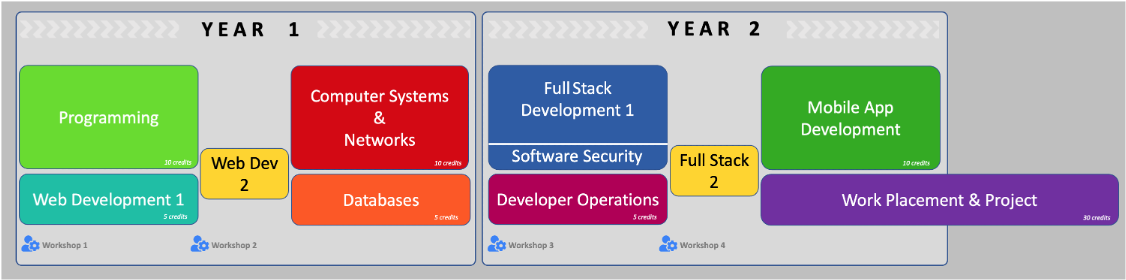
\includegraphics[width=19cm]{../common_images/orig/hdip_struct}}

\vspace{9pt}

As an accelerated course, there is an average time commitment of 16 hours per week required. Students with less ICT experience may need to factor in more time. The course is delivered using our award-winning online delivery platform---TutorStack. Pioneered on this programme with industry, we follow an ``Agile Semester'' approach, typically consisting of 4, three-week sprints followed by 1-week breaks for retrospective, after each sprint.

\vspace{12pt}
\mbox{}\hfill
\begin{minipage}{.32\textwidth}
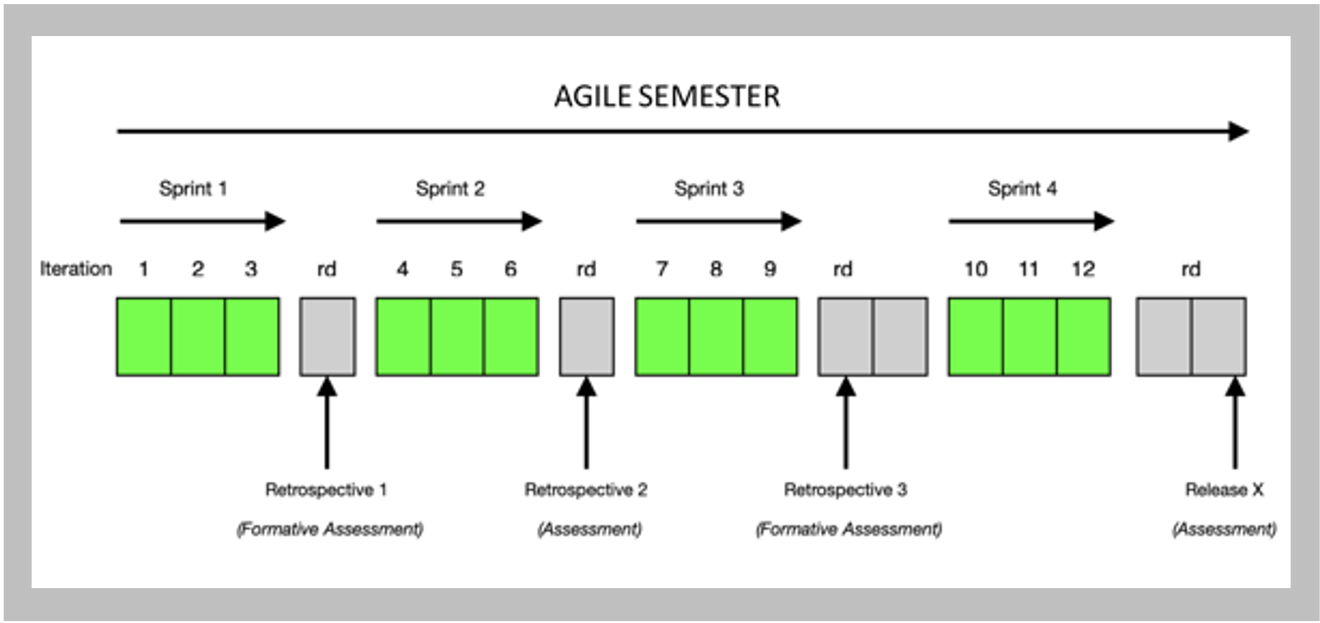
\includegraphics[width=\textwidth]{../common_images/orig/hdip_agile}
\end{minipage}\hfill
\begin{minipage}{.56\textwidth}
In addition there is a six lesson on-demand module each summer. Online delivery over the two years is supplemented by four onsite workshops to further enhance and deepen the learning experience, and learning community. Although not mandatory, these should be deemed essential. While all taught modules are delivered within two years, Work Project \& Placement runs into the following year so as not to over burden students.

\vspace{9pt}
For a more in depth preview of the course content and structure, please watch this 
\href{https://youtu.be/opRwmuwbf0I}{video}.

\vspace{9pt}
Try out a sample of the course \href{https://wit-hdip-comp-sci.github.io/}{here}.

\vspace{9pt}
\href{https:/www.wit.ie/courses/hdip-computer-science-parttime}{Find out more here}.

\vspace{-12pt}
\end{minipage}\hfill
\clearpage

%\projectstoc

%\clearpage
%\begin{center}
%\typesetPhotoTOC{6}{3.25cm}
%\end{center}

%\clearpage

%\typesetPhotoTOCGROUPS{6}{3cm}

%: projects

\projectsBegin


\input{../student_content/Leanne_Ahern_33484_content.tex}

\begingroup\globaldefs=1\relax

%: SID
\pgfkeyssetvalue{/students/Ludmila_Bulat_41BE2/SID}{[SID]}


%: Key
\def\Key{Ludmila_Bulat_41BE2}
\pgfkeyssetvalue{/students/Ludmila_Bulat_41BE2/Key}{Ludmila_Bulat_41BE2}

%: Name
\pgfkeyssetvalue{/students/Ludmila_Bulat_41BE2/Name}
{Ludmila Bulat}
\pgfkeyssetvalue{/students/Ludmila_Bulat_41BE2/SortName}
{Bulat, Ludmila}

%: Programme
\pgfkeyssetvalue{/students/Ludmila_Bulat_41BE2/Programme}
{Higher Diploma in Science in Computer Science}

%: Photo
\pgfkeyssetvalue{/students/Ludmila_Bulat_41BE2/Photo}
{Ludmila_Bulat_41BE2}
\pgfkeyssetvalue{/students/Ludmila_Bulat_41BE2/HasPhoto}
{True}

%: Poster
\pgfkeyssetvalue{/students/Ludmila_Bulat_41BE2/Poster}
{Ludmila_Bulat_41BE2}
\pgfkeyssetvalue{/students/Ludmila_Bulat_41BE2/HasPoster}
{True}
\pgfkeyssetvalue{/students/Ludmila_Bulat_41BE2/PosterWidth}
{3508}
\pgfkeyssetvalue{/students/Ludmila_Bulat_41BE2/PosterHeight}
{2480}
\pgfkeyssetvalue{/students/Ludmila_Bulat_41BE2/PosterOrientation}
{landscape}
\pgfkeyssetvalue{/students/Ludmila_Bulat_41BE2/PosterScale}
{0.9901612903225806}

%: QR
\pgfkeyssetvalue{/students/Ludmila_Bulat_41BE2/QR}
{SD}
\pgfkeyssetvalue{/students/Ludmila_Bulat_41BE2/HasQR}
{True}

%: CommercialTitle
\pgfkeyssetvalue{/students/Ludmila_Bulat_41BE2/CommercialTitle}
{ScanIQ}

%: AcademicTitle
\pgfkeyssetvalue{/students/Ludmila_Bulat_41BE2/AcademicTitle}
{Scaniq: A Mobile Application for Ingredient Analysis Using Barcode Scanning and Food Data APIs}

%: Summary
\pgfkeyssetvalue{/students/Ludmila_Bulat_41BE2/Summary}
{ScanIQ is a mobile application that helps users better understand food products by scanning barcodes and analysing ingredient data. The app integrates the OpenFoodFacts API to retrieve product information and applies a custom scoring system based on nutritional values such as sugar, salt, additives, and fibre. Users receive a simple colour-coded score and clear explanations, along with healthier product recommendations. The application also includes features such as scan history and favourites, focusing on usability, transparency, and informed decision-making.}

%: Technologies 
\pgfkeyssetvalue{/students/Ludmila_Bulat_41BE2/Technologies}
{React Native, Expo, TypeScript, OpenFoodFacts API, AsyncStorage, Expo Camera}

%: ProjectURL
\pgfkeyssetvalue{/students/Ludmila_Bulat_41BE2/ProjectURL}
{https://scaniq-final-project.vercel.app/}

%: SupervisorLabel
\pgfkeyssetvalue{/students/Ludmila_Bulat_41BE2/SupervisorLabel}
{Project Supervisor}

%: SupervisorTitle
\pgfkeyssetvalue{/students/Ludmila_Bulat_41BE2/SupervisorTitle}
{}

%: Supervisor
\pgfkeyssetvalue{/students/Ludmila_Bulat_41BE2/Supervisor}
{Dave Drohan}

%: Room
\pgfkeyssetvalue{/students/Ludmila_Bulat_41BE2/Room}
{TL2.38}

%: Number
\pgfkeyssetvalue{/students/Ludmila_Bulat_41BE2/Number}
{73}

%: ProjectAreas
\pgfkeyssetvalue{/students/Ludmila_Bulat_41BE2/ProjectAreas}
{AI ML Development,Software Development Core,Software Development Front End,Software Development Mobile Hybrid,Personal Independent Project}
\pgfkeyssetvalue{/students/Ludmila_Bulat_41BE2/ProjectAreasTeX}
{\pgfkeysvalueof{/area/AI ML Development/Name}, \pgfkeysvalueof{/area/Personal Independent Project/Name}, Software Development: (Core / Front End / Mobile Hybrid)}
\pgfkeyssetvalue{/students/Ludmila_Bulat_41BE2/ProjectAreasTeX2}
{\pgfkeysvalueof{/area/AI ML Development/Name}, \pgfkeysvalueof{/area/Personal Independent Project/Name}, Software Development: (Core / Front End / Mobile Hybrid)}

\endgroup

\DefaultLayout

\input{../student_content/Nigel_Byrne_2BD13_content.tex}

\begingroup\globaldefs=1\relax

%: SID
\pgfkeyssetvalue{/students/Vincent_Byrne_15519/SID}{[SID]}


%: Key
\def\Key{Vincent_Byrne_15519}
\pgfkeyssetvalue{/students/Vincent_Byrne_15519/Key}{Vincent_Byrne_15519}

%: Name
\pgfkeyssetvalue{/students/Vincent_Byrne_15519/Name}
{Vincent Byrne}
\pgfkeyssetvalue{/students/Vincent_Byrne_15519/SortName}
{Byrne, Vincent}

%: Programme
\pgfkeyssetvalue{/students/Vincent_Byrne_15519/Programme}
{Higher Diploma in Science in Computer Science}

%: Photo
\pgfkeyssetvalue{/students/Vincent_Byrne_15519/Photo}
{Vincent_Byrne_15519}
\pgfkeyssetvalue{/students/Vincent_Byrne_15519/HasPhoto}
{True}

%: Poster
\pgfkeyssetvalue{/students/Vincent_Byrne_15519/Poster}
{Vincent_Byrne_15519}
\pgfkeyssetvalue{/students/Vincent_Byrne_15519/HasPoster}
{True}
\pgfkeyssetvalue{/students/Vincent_Byrne_15519/PosterWidth}
{1346}
\pgfkeyssetvalue{/students/Vincent_Byrne_15519/PosterHeight}
{992}
\pgfkeyssetvalue{/students/Vincent_Byrne_15519/PosterOrientation}
{landscape}
\pgfkeyssetvalue{/students/Vincent_Byrne_15519/PosterScale}
{0.949798387096774}

%: QR
\pgfkeyssetvalue{/students/Vincent_Byrne_15519/QR}
{SD}
\pgfkeyssetvalue{/students/Vincent_Byrne_15519/HasQR}
{True}

%: CommercialTitle
\pgfkeyssetvalue{/students/Vincent_Byrne_15519/CommercialTitle}
{APAVS}

%: AcademicTitle
\pgfkeyssetvalue{/students/Vincent_Byrne_15519/AcademicTitle}
{Automated Pipeline and Visualisation System for Tool Load Port Data}

%: Summary
\pgfkeyssetvalue{/students/Vincent_Byrne_15519/Summary}
{APAVS automates the monitoring of load port qualification data across a fleet of semiconductor manufacturing tools. Currently, technicians manually export log files, run Excel macros, and visually inspect qualification plots for individual tools with no fleet-wide visibility. APAVS replaces this workflow with a PowerShell extraction pipeline that retrieves data directly from tool hard drives, parses raw sensor logs, and calculates slot-level offsets against taught reference positions. Results are stored in a SQL Server database and visualised through a Power BI.}

%: Technologies 
\pgfkeyssetvalue{/students/Vincent_Byrne_15519/Technologies}
{PowerShell, SQL Server, Power BI}

%: ProjectURL
\pgfkeyssetvalue{/students/Vincent_Byrne_15519/ProjectURL}
{https://bit.ly/4rJabZx}

%: SupervisorLabel
\pgfkeyssetvalue{/students/Vincent_Byrne_15519/SupervisorLabel}
{Project Supervisor}

%: SupervisorTitle
\pgfkeyssetvalue{/students/Vincent_Byrne_15519/SupervisorTitle}
{}

%: Supervisor
\pgfkeyssetvalue{/students/Vincent_Byrne_15519/Supervisor}
{Sonya Hogan}

%: Room
\pgfkeyssetvalue{/students/Vincent_Byrne_15519/Room}
{Not Presenting}

%: Number
\pgfkeyssetvalue{/students/Vincent_Byrne_15519/Number}
{75}

%: ProjectAreas
\pgfkeyssetvalue{/students/Vincent_Byrne_15519/ProjectAreas}
{Automotive and Automation,Database and Analytics,Work Based Project}
\pgfkeyssetvalue{/students/Vincent_Byrne_15519/ProjectAreasTeX}
{\pgfkeysvalueof{/area/Automotive and Automation/Name}, \pgfkeysvalueof{/area/Database and Analytics/Name}, \pgfkeysvalueof{/area/Work Based Project/Name}}
\pgfkeyssetvalue{/students/Vincent_Byrne_15519/ProjectAreasTeX2}
{\pgfkeysvalueof{/area/Automotive and Automation/Name}, \pgfkeysvalueof{/area/Database and Analytics/Name}, \pgfkeysvalueof{/area/Work Based Project/Name}}

\endgroup

\DefaultLayout

\input{../student_content/Peter_Chuk_1049E_content.tex}
\input{../student_content/Aidan_Clancy_92AB6_content.tex}
\input{../student_content/Shane_Crowley_E9668_content.tex}
\input{../student_content/Daniel_Cullen_9BC37_content.tex}
\input{../student_content/Eoin_Geoghegan_98F46_content.tex}

\begingroup\globaldefs=1\relax

%: SID
\pgfkeyssetvalue{/students/Wolfgang_Helnwein_16881/SID}{[SID]}


%: Key
\def\Key{Wolfgang_Helnwein_16881}
\pgfkeyssetvalue{/students/Wolfgang_Helnwein_16881/Key}{Wolfgang_Helnwein_16881}

%: Name
\pgfkeyssetvalue{/students/Wolfgang_Helnwein_16881/Name}
{Wolfgang Helnwein}
\pgfkeyssetvalue{/students/Wolfgang_Helnwein_16881/SortName}
{Helnwein, Wolfgang}

%: Programme
\pgfkeyssetvalue{/students/Wolfgang_Helnwein_16881/Programme}
{Higher Diploma in Science in Computer Science}

%: Photo
\pgfkeyssetvalue{/students/Wolfgang_Helnwein_16881/Photo}
{Wolfgang_Helnwein_16881}
\pgfkeyssetvalue{/students/Wolfgang_Helnwein_16881/HasPhoto}
{True}

%: Poster
\pgfkeyssetvalue{/students/Wolfgang_Helnwein_16881/Poster}
{Wolfgang_Helnwein_16881}
\pgfkeyssetvalue{/students/Wolfgang_Helnwein_16881/HasPoster}
{True}
\pgfkeyssetvalue{/students/Wolfgang_Helnwein_16881/PosterWidth}
{3508}
\pgfkeyssetvalue{/students/Wolfgang_Helnwein_16881/PosterHeight}
{2480}
\pgfkeyssetvalue{/students/Wolfgang_Helnwein_16881/PosterOrientation}
{landscape}
\pgfkeyssetvalue{/students/Wolfgang_Helnwein_16881/PosterScale}
{0.9901612903225806}

%: QR
\pgfkeyssetvalue{/students/Wolfgang_Helnwein_16881/QR}
{SD}
\pgfkeyssetvalue{/students/Wolfgang_Helnwein_16881/HasQR}
{True}

%: CommercialTitle
\pgfkeyssetvalue{/students/Wolfgang_Helnwein_16881/CommercialTitle}
{There's No Place Like Home}

%: AcademicTitle
\pgfkeyssetvalue{/students/Wolfgang_Helnwein_16881/AcademicTitle}
{Design and Implementation of a Segmented, Privacy-Centric Homelab Using Open-Source Platforms}

%: Summary
\pgfkeyssetvalue{/students/Wolfgang_Helnwein_16881/Summary}
{'There's No Place Like Home' shows how a typical home network can become a secure, scalable, privacy-focused homelab using open-source tools. It employs VLAN-based segmentation, a custom OPNsense router, a managed switch, and Proxmox for self-hosting to enable network isolation and flexible service deployment. Focused on hands-on learning, the project develops systems administration and architecture skills through iterative, experiential practice. Favouring locally hosted services and recycled hardware, it also demonstrates how individuals can cut cloud dependence and reduce electronic waste.}

%: Technologies 
\pgfkeyssetvalue{/students/Wolfgang_Helnwein_16881/Technologies}
{FreeBSD, OPNsense, Linux, Proxmox VE, Containers, Podman, Networking, Firewalls, VLANs}

%: ProjectURL
\pgfkeyssetvalue{/students/Wolfgang_Helnwein_16881/ProjectURL}
{https://urlr.me/!homelab}

%: SupervisorLabel
\pgfkeyssetvalue{/students/Wolfgang_Helnwein_16881/SupervisorLabel}
{Project Supervisor}

%: SupervisorTitle
\pgfkeyssetvalue{/students/Wolfgang_Helnwein_16881/SupervisorTitle}
{}

%: Supervisor
\pgfkeyssetvalue{/students/Wolfgang_Helnwein_16881/Supervisor}
{Mary Fitzgerald}

%: Room
\pgfkeyssetvalue{/students/Wolfgang_Helnwein_16881/Room}
{TL2.38}

%: Number
\pgfkeyssetvalue{/students/Wolfgang_Helnwein_16881/Number}
{81}

%: ProjectAreas
\pgfkeyssetvalue{/students/Wolfgang_Helnwein_16881/ProjectAreas}
{Computer Networks,DevOps,Information Systems and Modelling,Personal Independent Project,Open Source}
\pgfkeyssetvalue{/students/Wolfgang_Helnwein_16881/ProjectAreasTeX}
{\pgfkeysvalueof{/area/Computer Networks/Name}, \pgfkeysvalueof{/area/DevOps/Name}, \pgfkeysvalueof{/area/Information Systems and Modelling/Name}, \pgfkeysvalueof{/area/Personal Independent Project/Name}, \pgfkeysvalueof{/area/Open Source/Name}}
\pgfkeyssetvalue{/students/Wolfgang_Helnwein_16881/ProjectAreasTeX2}
{\pgfkeysvalueof{/area/Computer Networks/Name}, \pgfkeysvalueof{/area/DevOps/Name}, \pgfkeysvalueof{/area/Information Systems and Modelling/Name}, \pgfkeysvalueof{/area/Personal Independent Project/Name}, \pgfkeysvalueof{/area/Open Source/Name}}

\endgroup

\DefaultLayout


\begingroup\globaldefs=1\relax

%: SID
\pgfkeyssetvalue{/students/Oisin_Larkin_10A0F/SID}{[SID]}


%: Key
\def\Key{Oisin_Larkin_10A0F}
\pgfkeyssetvalue{/students/Oisin_Larkin_10A0F/Key}{Oisin_Larkin_10A0F}

%: Name
\pgfkeyssetvalue{/students/Oisin_Larkin_10A0F/Name}
{Oisin Larkin}
\pgfkeyssetvalue{/students/Oisin_Larkin_10A0F/SortName}
{Larkin, Oisin}

%: Programme
\pgfkeyssetvalue{/students/Oisin_Larkin_10A0F/Programme}
{Higher Diploma in Science in Computer Science}

%: Photo
\pgfkeyssetvalue{/students/Oisin_Larkin_10A0F/Photo}
{Oisin_Larkin_10A0F}
\pgfkeyssetvalue{/students/Oisin_Larkin_10A0F/HasPhoto}
{True}

%: Poster
\pgfkeyssetvalue{/students/Oisin_Larkin_10A0F/Poster}
{Oisin_Larkin_10A0F}
\pgfkeyssetvalue{/students/Oisin_Larkin_10A0F/HasPoster}
{True}
\pgfkeyssetvalue{/students/Oisin_Larkin_10A0F/PosterWidth}
{2480}
\pgfkeyssetvalue{/students/Oisin_Larkin_10A0F/PosterHeight}
{3508}
\pgfkeyssetvalue{/students/Oisin_Larkin_10A0F/PosterOrientation}
{portrait}
\pgfkeyssetvalue{/students/Oisin_Larkin_10A0F/PosterScale}
{1}

%: QR
\pgfkeyssetvalue{/students/Oisin_Larkin_10A0F/QR}
{SD}
\pgfkeyssetvalue{/students/Oisin_Larkin_10A0F/HasQR}
{True}

%: CommercialTitle
\pgfkeyssetvalue{/students/Oisin_Larkin_10A0F/CommercialTitle}
{CoRaw}

%: AcademicTitle
\pgfkeyssetvalue{/students/Oisin_Larkin_10A0F/AcademicTitle}
{Web App Designed to Help Users Learn and Practice Conversational Irish Using AI and Meta-prompting}

%: Summary
\pgfkeyssetvalue{/students/Oisin_Larkin_10A0F/Summary}
{CoRaw is a webapp designed to help users learn and practice conversational Irish using AI and meta-prompting. The webapp will take the user through immersive realistic conversations that will translate to improving real world conversational skills in Irish. The idea is that CoRaw will give people who are learning the Irish language a chance to engage in realistic everyday conversations at their own pace with an AI model. Users will be presented with some questions when they first login to determine their level and topics they are interested in.}

%: Technologies 
\pgfkeyssetvalue{/students/Oisin_Larkin_10A0F/Technologies}
{React, Hapi, Joi, JWT, Typescript}

%: ProjectURL
\pgfkeyssetvalue{/students/Oisin_Larkin_10A0F/ProjectURL}
{https://bit.ly/47h7xDa}

%: SupervisorLabel
\pgfkeyssetvalue{/students/Oisin_Larkin_10A0F/SupervisorLabel}
{Project Supervisor}

%: SupervisorTitle
\pgfkeyssetvalue{/students/Oisin_Larkin_10A0F/SupervisorTitle}
{}

%: Supervisor
\pgfkeyssetvalue{/students/Oisin_Larkin_10A0F/Supervisor}
{Michael McMahon}

%: Room
\pgfkeyssetvalue{/students/Oisin_Larkin_10A0F/Room}
{Not Presenting}

%: Number
\pgfkeyssetvalue{/students/Oisin_Larkin_10A0F/Number}
{82}

%: ProjectAreas
\pgfkeyssetvalue{/students/Oisin_Larkin_10A0F/ProjectAreas}
{Software Development Back End,Software Development Front End,Software Development Web,Personal Independent Project}
\pgfkeyssetvalue{/students/Oisin_Larkin_10A0F/ProjectAreasTeX}
{\pgfkeysvalueof{/area/Personal Independent Project/Name}, Software Development: (Back End / Front End / Web)}
\pgfkeyssetvalue{/students/Oisin_Larkin_10A0F/ProjectAreasTeX2}
{\pgfkeysvalueof{/area/Personal Independent Project/Name}, Software Development: (Back End / Front End / Web)}

\endgroup

\DefaultLayout

\input{../student_content/Garret_Lenihan_AD022_content.tex}
\input{../student_content/Conor_Leonard_63B89_content.tex}

\begingroup\globaldefs=1\relax

%: SID
\pgfkeyssetvalue{/students/Noemi_Lovei_FC73B/SID}{[SID]}


%: Key
\def\Key{Noemi_Lovei_FC73B}
\pgfkeyssetvalue{/students/Noemi_Lovei_FC73B/Key}{Noemi_Lovei_FC73B}

%: Name
\pgfkeyssetvalue{/students/Noemi_Lovei_FC73B/Name}
{Noemi Lovei}
\pgfkeyssetvalue{/students/Noemi_Lovei_FC73B/SortName}
{Lovei, Noemi}

%: Programme
\pgfkeyssetvalue{/students/Noemi_Lovei_FC73B/Programme}
{Higher Diploma in Science in Computer Science}

%: Photo
\pgfkeyssetvalue{/students/Noemi_Lovei_FC73B/Photo}
{Noemi_Lovei_FC73B}
\pgfkeyssetvalue{/students/Noemi_Lovei_FC73B/HasPhoto}
{True}

%: Poster
\pgfkeyssetvalue{/students/Noemi_Lovei_FC73B/Poster}
{Noemi_Lovei_FC73B}
\pgfkeyssetvalue{/students/Noemi_Lovei_FC73B/HasPoster}
{True}
\pgfkeyssetvalue{/students/Noemi_Lovei_FC73B/PosterWidth}
{746}
\pgfkeyssetvalue{/students/Noemi_Lovei_FC73B/PosterHeight}
{419}
\pgfkeyssetvalue{/students/Noemi_Lovei_FC73B/PosterOrientation}
{landscape}
\pgfkeyssetvalue{/students/Noemi_Lovei_FC73B/PosterScale}
{1}

%: QR
\pgfkeyssetvalue{/students/Noemi_Lovei_FC73B/QR}
{SD}
\pgfkeyssetvalue{/students/Noemi_Lovei_FC73B/HasQR}
{True}

%: CommercialTitle
\pgfkeyssetvalue{/students/Noemi_Lovei_FC73B/CommercialTitle}
{Done!}

%: AcademicTitle
\pgfkeyssetvalue{/students/Noemi_Lovei_FC73B/AcademicTitle}
{A Gamified Tracker of All Things Done Available on a Web App}

%: Summary
\pgfkeyssetvalue{/students/Noemi_Lovei_FC73B/Summary}
{A gamified tracker of all things done available on a webapp, supplemented with in-game currency and in-app statistics and charts for visualising user engagement. Built with a nodejs backend exposing the backend APIs, storing data through a MYSQL database and a react frontend all the while connected to a custom python mini AI server making recommendations based on user activity and delivering through web API. Built with robust front-end design, keeping data security and good database practices in mind.}

%: Technologies 
\pgfkeyssetvalue{/students/Noemi_Lovei_FC73B/Technologies}
{React, Nodejs, Python, Javascript, Typescript}

%: ProjectURL
\pgfkeyssetvalue{/students/Noemi_Lovei_FC73B/ProjectURL}
{https://nilanoemi25.github.io/project-/}

%: SupervisorLabel
\pgfkeyssetvalue{/students/Noemi_Lovei_FC73B/SupervisorLabel}
{Project Supervisor}

%: SupervisorTitle
\pgfkeyssetvalue{/students/Noemi_Lovei_FC73B/SupervisorTitle}
{}

%: Supervisor
\pgfkeyssetvalue{/students/Noemi_Lovei_FC73B/Supervisor}
{Richard Lacey}

%: Room
\pgfkeyssetvalue{/students/Noemi_Lovei_FC73B/Room}
{Not Presenting}

%: Number
\pgfkeyssetvalue{/students/Noemi_Lovei_FC73B/Number}
{85}

%: ProjectAreas
\pgfkeyssetvalue{/students/Noemi_Lovei_FC73B/ProjectAreas}
{Software Development Back End,Software Development Front End,Personal Independent Project}
\pgfkeyssetvalue{/students/Noemi_Lovei_FC73B/ProjectAreasTeX}
{\pgfkeysvalueof{/area/Personal Independent Project/Name}, Software Development: (Back End / Front End)}
\pgfkeyssetvalue{/students/Noemi_Lovei_FC73B/ProjectAreasTeX2}
{\pgfkeysvalueof{/area/Personal Independent Project/Name}, Software Development: (Back End / Front End)}

\endgroup

\DefaultLayout

\input{../student_content/Rhiannah_Maher_DAB99_content.tex}

\begingroup\globaldefs=1\relax

%: SID
\pgfkeyssetvalue{/students/Fergal_McLoughlan_84A24/SID}{[SID]}


%: Key
\def\Key{Fergal_McLoughlan_84A24}
\pgfkeyssetvalue{/students/Fergal_McLoughlan_84A24/Key}{Fergal_McLoughlan_84A24}

%: Name
\pgfkeyssetvalue{/students/Fergal_McLoughlan_84A24/Name}
{Fergal McLoughlan}
\pgfkeyssetvalue{/students/Fergal_McLoughlan_84A24/SortName}
{McLoughlan, Fergal}

%: Programme
\pgfkeyssetvalue{/students/Fergal_McLoughlan_84A24/Programme}
{Higher Diploma in Science in Computer Science}

%: Photo
\pgfkeyssetvalue{/students/Fergal_McLoughlan_84A24/Photo}
{Fergal_McLoughlan_84A24}
\pgfkeyssetvalue{/students/Fergal_McLoughlan_84A24/HasPhoto}
{True}

%: Poster
\pgfkeyssetvalue{/students/Fergal_McLoughlan_84A24/Poster}
{Fergal_McLoughlan_84A24}
\pgfkeyssetvalue{/students/Fergal_McLoughlan_84A24/HasPoster}
{True}
\pgfkeyssetvalue{/students/Fergal_McLoughlan_84A24/PosterWidth}
{1916}
\pgfkeyssetvalue{/students/Fergal_McLoughlan_84A24/PosterHeight}
{968}
\pgfkeyssetvalue{/students/Fergal_McLoughlan_84A24/PosterOrientation}
{landscape}
\pgfkeyssetvalue{/students/Fergal_McLoughlan_84A24/PosterScale}
{1}

%: QR
\pgfkeyssetvalue{/students/Fergal_McLoughlan_84A24/QR}
{SD}
\pgfkeyssetvalue{/students/Fergal_McLoughlan_84A24/HasQR}
{True}

%: CommercialTitle
\pgfkeyssetvalue{/students/Fergal_McLoughlan_84A24/CommercialTitle}
{ECADS}

%: AcademicTitle
\pgfkeyssetvalue{/students/Fergal_McLoughlan_84A24/AcademicTitle}
{Emergency Services Contact \& Dispatch System for Offline Incident Management}

%: Summary
\pgfkeyssetvalue{/students/Fergal_McLoughlan_84A24/Summary}
{An offline stand-alone contact and dispatch system designed for the emergency services, Gardaí in particular, to allow data capture of call information and incident management in a \textquotedblleft{}system/network down\textquotedblright{} scenario.
ECADS has been developed from a simple interactive Bash and PowerShell script version into a graphical Windows Forms application which records data at a local level on individual clients. This makes it a lightweight solution which is easily deployable on control room clients or local servers, depending on the size of the control room.}

%: Technologies 
\pgfkeyssetvalue{/students/Fergal_McLoughlan_84A24/Technologies}
{Bash, PowerShell, C\#, Windows Forms}

%: ProjectURL
\pgfkeyssetvalue{/students/Fergal_McLoughlan_84A24/ProjectURL}
{https://feargalmcloughlin.github.io/ECADS/}

%: SupervisorLabel
\pgfkeyssetvalue{/students/Fergal_McLoughlan_84A24/SupervisorLabel}
{Project Supervisor}

%: SupervisorTitle
\pgfkeyssetvalue{/students/Fergal_McLoughlan_84A24/SupervisorTitle}
{}

%: Supervisor
\pgfkeyssetvalue{/students/Fergal_McLoughlan_84A24/Supervisor}
{Dr Sinead O'Neill}

%: Room
\pgfkeyssetvalue{/students/Fergal_McLoughlan_84A24/Room}
{Not Presenting}

%: Number
\pgfkeyssetvalue{/students/Fergal_McLoughlan_84A24/Number}
{87}

%: ProjectAreas
\pgfkeyssetvalue{/students/Fergal_McLoughlan_84A24/ProjectAreas}
{Software Development Core,Personal Independent Project}
\pgfkeyssetvalue{/students/Fergal_McLoughlan_84A24/ProjectAreasTeX}
{\pgfkeysvalueof{/area/Personal Independent Project/Name}, Software Development: (Core)}
\pgfkeyssetvalue{/students/Fergal_McLoughlan_84A24/ProjectAreasTeX2}
{\pgfkeysvalueof{/area/Personal Independent Project/Name}, Software Development: (Core)}

\endgroup

\DefaultLayout


\begingroup\globaldefs=1\relax

%: SID
\pgfkeyssetvalue{/students/Vadym_Melnychenko_C2F50/SID}{[SID]}


%: Key
\def\Key{Vadym_Melnychenko_C2F50}
\pgfkeyssetvalue{/students/Vadym_Melnychenko_C2F50/Key}{Vadym_Melnychenko_C2F50}

%: Name
\pgfkeyssetvalue{/students/Vadym_Melnychenko_C2F50/Name}
{Vadym Melnychenko}
\pgfkeyssetvalue{/students/Vadym_Melnychenko_C2F50/SortName}
{Melnychenko, Vadym}

%: Programme
\pgfkeyssetvalue{/students/Vadym_Melnychenko_C2F50/Programme}
{Higher Diploma in Science in Computer Science}

%: Photo
\pgfkeyssetvalue{/students/Vadym_Melnychenko_C2F50/Photo}
{Vadym_Melnychenko_C2F50}
\pgfkeyssetvalue{/students/Vadym_Melnychenko_C2F50/HasPhoto}
{True}

%: Poster
\pgfkeyssetvalue{/students/Vadym_Melnychenko_C2F50/Poster}
{Vadym_Melnychenko_C2F50}
\pgfkeyssetvalue{/students/Vadym_Melnychenko_C2F50/HasPoster}
{True}
\pgfkeyssetvalue{/students/Vadym_Melnychenko_C2F50/PosterWidth}
{1600}
\pgfkeyssetvalue{/students/Vadym_Melnychenko_C2F50/PosterHeight}
{1877}
\pgfkeyssetvalue{/students/Vadym_Melnychenko_C2F50/PosterOrientation}
{portrait}
\pgfkeyssetvalue{/students/Vadym_Melnychenko_C2F50/PosterScale}
{1}

%: QR
\pgfkeyssetvalue{/students/Vadym_Melnychenko_C2F50/QR}
{SD}
\pgfkeyssetvalue{/students/Vadym_Melnychenko_C2F50/HasQR}
{True}

%: CommercialTitle
\pgfkeyssetvalue{/students/Vadym_Melnychenko_C2F50/CommercialTitle}
{Wynsum Point of Sale}

%: AcademicTitle
\pgfkeyssetvalue{/students/Vadym_Melnychenko_C2F50/AcademicTitle}
{A High-Performance Edge-Native Point of Sale Terminal with Zero Trust Security}

%: Summary
\pgfkeyssetvalue{/students/Vadym_Melnychenko_C2F50/Summary}
{This project delivered Wynsum POS, a high-performance PWA within an Edge-Native RMS. It bridges the gap between complex marketing needs and legacy infrastructure. Redefining performance for retail, the system eschews traditional caching to ensure 100\% data consistency. Using a WebSocket-based JSON-RPC protocol and row virtualization, it manages 10,000+ items at 60 FPS. Adhering to \textquotedblleft{}Zero Trust,\textquotedblright{} all financial logic is server-side and secured via ECDSA hardware keys. An Asynchronous Checkout Pipeline ensures sub-5ms response times during complex multi-step retail transactions.}

%: Technologies 
\pgfkeyssetvalue{/students/Vadym_Melnychenko_C2F50/Technologies}
{Python, Django, Django Channels, Daphne/Uvicorn, Redis, PostgreSQL, React, Vite, TypeScript}

%: ProjectURL
\pgfkeyssetvalue{/students/Vadym_Melnychenko_C2F50/ProjectURL}
{https://project.wynsum.ie/}

%: SupervisorLabel
\pgfkeyssetvalue{/students/Vadym_Melnychenko_C2F50/SupervisorLabel}
{Project Supervisor}

%: SupervisorTitle
\pgfkeyssetvalue{/students/Vadym_Melnychenko_C2F50/SupervisorTitle}
{}

%: Supervisor
\pgfkeyssetvalue{/students/Vadym_Melnychenko_C2F50/Supervisor}
{Michael McMahon}

%: Room
\pgfkeyssetvalue{/students/Vadym_Melnychenko_C2F50/Room}
{Not Presenting}

%: Number
\pgfkeyssetvalue{/students/Vadym_Melnychenko_C2F50/Number}
{88}

%: ProjectAreas
\pgfkeyssetvalue{/students/Vadym_Melnychenko_C2F50/ProjectAreas}
{Software Development Back End,Software Development Core,Software Development Front End,Software Development Web,Personal Independent Project}
\pgfkeyssetvalue{/students/Vadym_Melnychenko_C2F50/ProjectAreasTeX}
{\pgfkeysvalueof{/area/Personal Independent Project/Name}, Software Development: (Back End / Core / Front End / Web)}
\pgfkeyssetvalue{/students/Vadym_Melnychenko_C2F50/ProjectAreasTeX2}
{\pgfkeysvalueof{/area/Personal Independent Project/Name}, Software Development: (Back End / Core / Front End / Web)}

\endgroup

\DefaultLayout


\begingroup\globaldefs=1\relax

%: SID
\pgfkeyssetvalue{/students/Jake_Nagle_82BC6/SID}{[SID]}


%: Key
\def\Key{Jake_Nagle_82BC6}
\pgfkeyssetvalue{/students/Jake_Nagle_82BC6/Key}{Jake_Nagle_82BC6}

%: Name
\pgfkeyssetvalue{/students/Jake_Nagle_82BC6/Name}
{Jake Nagle}
\pgfkeyssetvalue{/students/Jake_Nagle_82BC6/SortName}
{Nagle, Jake}

%: Programme
\pgfkeyssetvalue{/students/Jake_Nagle_82BC6/Programme}
{Higher Diploma in Science in Computer Science}

%: Photo
\pgfkeyssetvalue{/students/Jake_Nagle_82BC6/Photo}
{Jake_Nagle_82BC6}
\pgfkeyssetvalue{/students/Jake_Nagle_82BC6/HasPhoto}
{True}

%: Poster
\pgfkeyssetvalue{/students/Jake_Nagle_82BC6/Poster}
{Jake_Nagle_82BC6}
\pgfkeyssetvalue{/students/Jake_Nagle_82BC6/HasPoster}
{True}
\pgfkeyssetvalue{/students/Jake_Nagle_82BC6/PosterWidth}
{1280}
\pgfkeyssetvalue{/students/Jake_Nagle_82BC6/PosterHeight}
{720}
\pgfkeyssetvalue{/students/Jake_Nagle_82BC6/PosterOrientation}
{landscape}
\pgfkeyssetvalue{/students/Jake_Nagle_82BC6/PosterScale}
{1}

%: QR
\pgfkeyssetvalue{/students/Jake_Nagle_82BC6/QR}
{SD}
\pgfkeyssetvalue{/students/Jake_Nagle_82BC6/HasQR}
{True}

%: CommercialTitle
\pgfkeyssetvalue{/students/Jake_Nagle_82BC6/CommercialTitle}
{EVOTE}

%: AcademicTitle
\pgfkeyssetvalue{/students/Jake_Nagle_82BC6/AcademicTitle}
{An Electronic Voting System Implemented as a Full Stack Application Addressing UI for Disabilities}

%: Summary
\pgfkeyssetvalue{/students/Jake_Nagle_82BC6/Summary}
{This project is a full-stack web application simulating a secure and accessible electronic voting system. Users can register, log in, and cast a vote. The frontend is built on Visual Studio Code with Angular, the backend with Visual Studio using C\#, and SQL Server Management 22 is used for database. An admin panel allows management of users, candidates, elections, and viewing vote analytics. Security is implemented using JWT tokens and hashing of user passwords. The system implements accessibility features to support users with reading and sight disabilities.}

%: Technologies 
\pgfkeyssetvalue{/students/Jake_Nagle_82BC6/Technologies}
{Visual Studio Code, Visual Studio, SQL Server Management 22}

%: ProjectURL
\pgfkeyssetvalue{/students/Jake_Nagle_82BC6/ProjectURL}
{https://jake-nagle123.github.io/EVoting/project.html}

%: SupervisorLabel
\pgfkeyssetvalue{/students/Jake_Nagle_82BC6/SupervisorLabel}
{Project Supervisor}

%: SupervisorTitle
\pgfkeyssetvalue{/students/Jake_Nagle_82BC6/SupervisorTitle}
{}

%: Supervisor
\pgfkeyssetvalue{/students/Jake_Nagle_82BC6/Supervisor}
{Catherine Fitzpatrick}

%: Room
\pgfkeyssetvalue{/students/Jake_Nagle_82BC6/Room}
{Not Presenting}

%: Number
\pgfkeyssetvalue{/students/Jake_Nagle_82BC6/Number}
{89}

%: ProjectAreas
\pgfkeyssetvalue{/students/Jake_Nagle_82BC6/ProjectAreas}
{Software Development Back End,Software Development Core,Software Development Front End,Software Development Web}
\pgfkeyssetvalue{/students/Jake_Nagle_82BC6/ProjectAreasTeX}
{Software Development: (Back End / Core / Front End / Web)}
\pgfkeyssetvalue{/students/Jake_Nagle_82BC6/ProjectAreasTeX2}
{Software Development: (Back End / Core / Front End / Web)}

\endgroup

\DefaultLayout


\begingroup\globaldefs=1\relax

%: SID
\pgfkeyssetvalue{/students/Andrea_Nardinocchi_EF120/SID}{[SID]}


%: Key
\def\Key{Andrea_Nardinocchi_EF120}
\pgfkeyssetvalue{/students/Andrea_Nardinocchi_EF120/Key}{Andrea_Nardinocchi_EF120}

%: Name
\pgfkeyssetvalue{/students/Andrea_Nardinocchi_EF120/Name}
{Andrea Nardinocchi}
\pgfkeyssetvalue{/students/Andrea_Nardinocchi_EF120/SortName}
{Nardinocchi, Andrea}

%: Programme
\pgfkeyssetvalue{/students/Andrea_Nardinocchi_EF120/Programme}
{Higher Diploma in Science in Computer Science}

%: Photo
\pgfkeyssetvalue{/students/Andrea_Nardinocchi_EF120/Photo}
{Andrea_Nardinocchi_EF120}
\pgfkeyssetvalue{/students/Andrea_Nardinocchi_EF120/HasPhoto}
{True}

%: Poster
\pgfkeyssetvalue{/students/Andrea_Nardinocchi_EF120/Poster}
{Andrea_Nardinocchi_EF120}
\pgfkeyssetvalue{/students/Andrea_Nardinocchi_EF120/HasPoster}
{True}
\pgfkeyssetvalue{/students/Andrea_Nardinocchi_EF120/PosterWidth}
{1366}
\pgfkeyssetvalue{/students/Andrea_Nardinocchi_EF120/PosterHeight}
{1223}
\pgfkeyssetvalue{/students/Andrea_Nardinocchi_EF120/PosterOrientation}
{landscape}
\pgfkeyssetvalue{/students/Andrea_Nardinocchi_EF120/PosterScale}
{0.7818479149632052}

%: QR
\pgfkeyssetvalue{/students/Andrea_Nardinocchi_EF120/QR}
{SD}
\pgfkeyssetvalue{/students/Andrea_Nardinocchi_EF120/HasQR}
{True}

%: CommercialTitle
\pgfkeyssetvalue{/students/Andrea_Nardinocchi_EF120/CommercialTitle}
{GuestEase}

%: AcademicTitle
\pgfkeyssetvalue{/students/Andrea_Nardinocchi_EF120/AcademicTitle}
{A Full-stack Web App for Small Hospitality Businesses}

%: Summary
\pgfkeyssetvalue{/students/Andrea_Nardinocchi_EF120/Summary}
{GuestEase is a full-stack web app designed for small hospitality businesses such as B\&B, guesthouses, and small boutique hotels. This booking system enables users to create and manage their bookings, profiles, write reviews, while also processing Stripe payments. It features an admin dashboard through which the administrator can create, and manage bookings, user accounts, manage rooms availability, and read users' reviews. It triggers email notifications, which can be cron-automated. Its goal is to provide a user-friendly tool to streamline the user experience on both ends: guests and admin.}

%: Technologies 
\pgfkeyssetvalue{/students/Andrea_Nardinocchi_EF120/Technologies}
{React, Vite, TypeScript, Material UI, Node.js \& Express, Supabase, Cron-job, Stripe, Resend}

%: ProjectURL
\pgfkeyssetvalue{/students/Andrea_Nardinocchi_EF120/ProjectURL}
{https://guestease-landing.vercel.app/}

%: SupervisorLabel
\pgfkeyssetvalue{/students/Andrea_Nardinocchi_EF120/SupervisorLabel}
{Project Supervisor}

%: SupervisorTitle
\pgfkeyssetvalue{/students/Andrea_Nardinocchi_EF120/SupervisorTitle}
{}

%: Supervisor
\pgfkeyssetvalue{/students/Andrea_Nardinocchi_EF120/Supervisor}
{Catherine Fitzpatrick}

%: Room
\pgfkeyssetvalue{/students/Andrea_Nardinocchi_EF120/Room}
{Not Presenting}

%: Number
\pgfkeyssetvalue{/students/Andrea_Nardinocchi_EF120/Number}
{90}

%: ProjectAreas
\pgfkeyssetvalue{/students/Andrea_Nardinocchi_EF120/ProjectAreas}
{Software Development Back End,Software Development Front End,Software Development Web,Personal Independent Project}
\pgfkeyssetvalue{/students/Andrea_Nardinocchi_EF120/ProjectAreasTeX}
{\pgfkeysvalueof{/area/Personal Independent Project/Name}, Software Development: (Back End / Front End / Web)}
\pgfkeyssetvalue{/students/Andrea_Nardinocchi_EF120/ProjectAreasTeX2}
{\pgfkeysvalueof{/area/Personal Independent Project/Name}, Software Development: (Back End / Front End / Web)}

\endgroup

\DefaultLayout

\input{../student_content/David_OConnor_24514_content.tex}
\input{../student_content/Grainne_OConnor_7B96B_content.tex}

\begingroup\globaldefs=1\relax

%: SID
\pgfkeyssetvalue{/students/Michael_ODriscoll_106C1/SID}{[SID]}


%: Key
\def\Key{Michael_ODriscoll_106C1}
\pgfkeyssetvalue{/students/Michael_ODriscoll_106C1/Key}{Michael_ODriscoll_106C1}

%: Name
\pgfkeyssetvalue{/students/Michael_ODriscoll_106C1/Name}
{Michael O'Driscoll}
\pgfkeyssetvalue{/students/Michael_ODriscoll_106C1/SortName}
{O'Driscoll, Michael}

%: Programme
\pgfkeyssetvalue{/students/Michael_ODriscoll_106C1/Programme}
{Higher Diploma in Science in Computer Science}

%: Photo
\pgfkeyssetvalue{/students/Michael_ODriscoll_106C1/Photo}
{Michael_ODriscoll_106C1}
\pgfkeyssetvalue{/students/Michael_ODriscoll_106C1/HasPhoto}
{True}

%: Poster
\pgfkeyssetvalue{/students/Michael_ODriscoll_106C1/Poster}
{Michael_ODriscoll_106C1}
\pgfkeyssetvalue{/students/Michael_ODriscoll_106C1/HasPoster}
{True}
\pgfkeyssetvalue{/students/Michael_ODriscoll_106C1/PosterWidth}
{2237}
\pgfkeyssetvalue{/students/Michael_ODriscoll_106C1/PosterHeight}
{2483}
\pgfkeyssetvalue{/students/Michael_ODriscoll_106C1/PosterOrientation}
{portrait}
\pgfkeyssetvalue{/students/Michael_ODriscoll_106C1/PosterScale}
{1}

%: QR
\pgfkeyssetvalue{/students/Michael_ODriscoll_106C1/QR}
{SD}
\pgfkeyssetvalue{/students/Michael_ODriscoll_106C1/HasQR}
{True}

%: CommercialTitle
\pgfkeyssetvalue{/students/Michael_ODriscoll_106C1/CommercialTitle}
{Odin}

%: AcademicTitle
\pgfkeyssetvalue{/students/Michael_ODriscoll_106C1/AcademicTitle}
{An Autonomous Cloud Infrastructure Management System}

%: Summary
\pgfkeyssetvalue{/students/Michael_ODriscoll_106C1/Summary}
{An autonomous cloud infrastructure system monitors EC2 instances on Amazon Web Services, analyzing and responding to operational events to ensure reliability, scalability, and resilience across multiple cloud instances. It continuously tracks key metrics such as CPU usage, memory consumption, network bandwidth, uptime, and database storage. An AI agent from OpenAI analyzes recent datasets to summarize overall system health, identify potential risks, and recommend corrective actions. All metrics, event logs, and AI insights are presented on a dashboard for monitoring and decision-making.}

%: Technologies 
\pgfkeyssetvalue{/students/Michael_ODriscoll_106C1/Technologies}
{AWS, Python, Node.js, Javascript, Handlebars, MongoDB, OpenAI}

%: ProjectURL
\pgfkeyssetvalue{/students/Michael_ODriscoll_106C1/ProjectURL}
{https://modrisco89.github.io/Odin/}

%: SupervisorLabel
\pgfkeyssetvalue{/students/Michael_ODriscoll_106C1/SupervisorLabel}
{Project Supervisor}

%: SupervisorTitle
\pgfkeyssetvalue{/students/Michael_ODriscoll_106C1/SupervisorTitle}
{}

%: Supervisor
\pgfkeyssetvalue{/students/Michael_ODriscoll_106C1/Supervisor}
{David Drohan}

%: Room
\pgfkeyssetvalue{/students/Michael_ODriscoll_106C1/Room}
{TL2.38}

%: Number
\pgfkeyssetvalue{/students/Michael_ODriscoll_106C1/Number}
{93}

%: ProjectAreas
\pgfkeyssetvalue{/students/Michael_ODriscoll_106C1/ProjectAreas}
{DevOps,Software Development Web,Personal Independent Project}
\pgfkeyssetvalue{/students/Michael_ODriscoll_106C1/ProjectAreasTeX}
{\pgfkeysvalueof{/area/DevOps/Name}, \pgfkeysvalueof{/area/Personal Independent Project/Name}, Software Development: (Web)}
\pgfkeyssetvalue{/students/Michael_ODriscoll_106C1/ProjectAreasTeX2}
{\pgfkeysvalueof{/area/DevOps/Name}, \pgfkeysvalueof{/area/Personal Independent Project/Name}, Software Development: (Web)}

\endgroup

\DefaultLayout


\begingroup\globaldefs=1\relax

%: SID
\pgfkeyssetvalue{/students/Joe_Power_48605/SID}{[SID]}


%: Key
\def\Key{Joe_Power_48605}
\pgfkeyssetvalue{/students/Joe_Power_48605/Key}{Joe_Power_48605}

%: Name
\pgfkeyssetvalue{/students/Joe_Power_48605/Name}
{Joe Power}
\pgfkeyssetvalue{/students/Joe_Power_48605/SortName}
{Power, Joe}

%: Programme
\pgfkeyssetvalue{/students/Joe_Power_48605/Programme}
{Higher Diploma in Science in Computer Science}

%: Photo
\pgfkeyssetvalue{/students/Joe_Power_48605/Photo}
{Joe_Power_48605}
\pgfkeyssetvalue{/students/Joe_Power_48605/HasPhoto}
{True}

%: Poster
\pgfkeyssetvalue{/students/Joe_Power_48605/Poster}
{Joe_Power_48605}
\pgfkeyssetvalue{/students/Joe_Power_48605/HasPoster}
{True}
\pgfkeyssetvalue{/students/Joe_Power_48605/PosterWidth}
{707}
\pgfkeyssetvalue{/students/Joe_Power_48605/PosterHeight}
{627}
\pgfkeyssetvalue{/students/Joe_Power_48605/PosterOrientation}
{landscape}
\pgfkeyssetvalue{/students/Joe_Power_48605/PosterScale}
{0.7893141945773524}

%: QR
\pgfkeyssetvalue{/students/Joe_Power_48605/QR}
{SD}
\pgfkeyssetvalue{/students/Joe_Power_48605/HasQR}
{True}

%: CommercialTitle
\pgfkeyssetvalue{/students/Joe_Power_48605/CommercialTitle}
{ANDROIDS}

%: AcademicTitle
\pgfkeyssetvalue{/students/Joe_Power_48605/AcademicTitle}
{Air Navigation Data for Radio Officer Information Display System}

%: Summary
\pgfkeyssetvalue{/students/Joe_Power_48605/Summary}
{An information display system for Radio Officers, providing HF and VHF radio frequencies, Weather data, NOTAMs for North Atlantic operations, with supplementary operational and engineering notes. The system is complemented by a Map view display system using leaflet and API data derived from the HAPI backend, Aviation ADSB feeds and NASA Space Weather. Phase I establishes a secure, validated, fully functional backend. Phase II builds a modern, interactive, map‑driven interface powered by Svelte and Leaflet.}

%: Technologies 
\pgfkeyssetvalue{/students/Joe_Power_48605/Technologies}
{Nodejs, hapi, mongoDB, Svelte, Leaflet}

%: ProjectURL
\pgfkeyssetvalue{/students/Joe_Power_48605/ProjectURL}
{https://powerj24.github.io/hdip24-project/}

%: SupervisorLabel
\pgfkeyssetvalue{/students/Joe_Power_48605/SupervisorLabel}
{Project Supervisor}

%: SupervisorTitle
\pgfkeyssetvalue{/students/Joe_Power_48605/SupervisorTitle}
{}

%: Supervisor
\pgfkeyssetvalue{/students/Joe_Power_48605/Supervisor}
{David Drohan}

%: Room
\pgfkeyssetvalue{/students/Joe_Power_48605/Room}
{Not Presenting}

%: Number
\pgfkeyssetvalue{/students/Joe_Power_48605/Number}
{94}

%: ProjectAreas
\pgfkeyssetvalue{/students/Joe_Power_48605/ProjectAreas}
{Software Development Web,Work Based Project}
\pgfkeyssetvalue{/students/Joe_Power_48605/ProjectAreasTeX}
{\pgfkeysvalueof{/area/Work Based Project/Name}, Software Development: (Web)}
\pgfkeyssetvalue{/students/Joe_Power_48605/ProjectAreasTeX2}
{\pgfkeysvalueof{/area/Work Based Project/Name}, Software Development: (Web)}

\endgroup

\DefaultLayout

\input{../student_content/Elaine_Rice_AA215_content.tex}

\begingroup\globaldefs=1\relax

%: SID
\pgfkeyssetvalue{/students/Pedro_Royo_636C3/SID}{[SID]}


%: Key
\def\Key{Pedro_Royo_636C3}
\pgfkeyssetvalue{/students/Pedro_Royo_636C3/Key}{Pedro_Royo_636C3}

%: Name
\pgfkeyssetvalue{/students/Pedro_Royo_636C3/Name}
{Pedro Royo}
\pgfkeyssetvalue{/students/Pedro_Royo_636C3/SortName}
{Royo, Pedro}

%: Programme
\pgfkeyssetvalue{/students/Pedro_Royo_636C3/Programme}
{Higher Diploma in Science in Computer Science}

%: Photo
\pgfkeyssetvalue{/students/Pedro_Royo_636C3/Photo}
{Pedro_Royo_636C3}
\pgfkeyssetvalue{/students/Pedro_Royo_636C3/HasPhoto}
{True}

%: Poster
\pgfkeyssetvalue{/students/Pedro_Royo_636C3/Poster}
{Pedro_Royo_636C3}
\pgfkeyssetvalue{/students/Pedro_Royo_636C3/HasPoster}
{True}
\pgfkeyssetvalue{/students/Pedro_Royo_636C3/PosterWidth}
{2480}
\pgfkeyssetvalue{/students/Pedro_Royo_636C3/PosterHeight}
{3508}
\pgfkeyssetvalue{/students/Pedro_Royo_636C3/PosterOrientation}
{portrait}
\pgfkeyssetvalue{/students/Pedro_Royo_636C3/PosterScale}
{1}

%: QR
\pgfkeyssetvalue{/students/Pedro_Royo_636C3/QR}
{SD}
\pgfkeyssetvalue{/students/Pedro_Royo_636C3/HasQR}
{True}

%: CommercialTitle
\pgfkeyssetvalue{/students/Pedro_Royo_636C3/CommercialTitle}
{Label Automator}

%: AcademicTitle
\pgfkeyssetvalue{/students/Pedro_Royo_636C3/AcademicTitle}
{3 Approaches to Designing EU Compliant Labels (Scripting, Coding and AI Prompting)}

%: Summary
\pgfkeyssetvalue{/students/Pedro_Royo_636C3/Summary}
{This project explores different ways to automate label design, particularly the initial steps of the design process. These steps include checking for compliance with European regulations and gathering each item of information that needs to appear on the label. Both tasks can be very time consuming and prone to error when done manually. 

The approaches researched include Adobe Illustrator scripting, Generative AI, and Python with Pandas library for data manipulation along typesetting with LaTeX. Suitable approaches may be effectively adopted into the design workflow.}

%: Technologies 
\pgfkeyssetvalue{/students/Pedro_Royo_636C3/Technologies}
{Javascript, Python, Pandas, LaTeX, AI}

%: ProjectURL
\pgfkeyssetvalue{/students/Pedro_Royo_636C3/ProjectURL}
{https://bit.ly/LabelAutomator}

%: SupervisorLabel
\pgfkeyssetvalue{/students/Pedro_Royo_636C3/SupervisorLabel}
{Project Supervisor}

%: SupervisorTitle
\pgfkeyssetvalue{/students/Pedro_Royo_636C3/SupervisorTitle}
{}

%: Supervisor
\pgfkeyssetvalue{/students/Pedro_Royo_636C3/Supervisor}
{Dr Mujahid Tabassum}

%: Room
\pgfkeyssetvalue{/students/Pedro_Royo_636C3/Room}
{Not Presenting}

%: Number
\pgfkeyssetvalue{/students/Pedro_Royo_636C3/Number}
{96}

%: ProjectAreas
\pgfkeyssetvalue{/students/Pedro_Royo_636C3/ProjectAreas}
{Automotive and Automation,Digital Graphic Design}
\pgfkeyssetvalue{/students/Pedro_Royo_636C3/ProjectAreasTeX}
{\pgfkeysvalueof{/area/Automotive and Automation/Name}, \pgfkeysvalueof{/area/Digital Graphic Design/Name}}
\pgfkeyssetvalue{/students/Pedro_Royo_636C3/ProjectAreasTeX2}
{\pgfkeysvalueof{/area/Automotive and Automation/Name}, \pgfkeysvalueof{/area/Digital Graphic Design/Name}}

\endgroup

\DefaultLayout

\input{../student_content/Giovanni_Serra_EDC5F_content.tex}
\input{../student_content/Marian_Sheehy_BF690_content.tex}

\begingroup\globaldefs=1\relax

%: SID
\pgfkeyssetvalue{/students/Joshua_Smiles_A86C7/SID}{[SID]}


%: Key
\def\Key{Joshua_Smiles_A86C7}
\pgfkeyssetvalue{/students/Joshua_Smiles_A86C7/Key}{Joshua_Smiles_A86C7}

%: Name
\pgfkeyssetvalue{/students/Joshua_Smiles_A86C7/Name}
{Joshua Smiles}
\pgfkeyssetvalue{/students/Joshua_Smiles_A86C7/SortName}
{Smiles, Joshua}

%: Programme
\pgfkeyssetvalue{/students/Joshua_Smiles_A86C7/Programme}
{Higher Diploma in Science in Computer Science}

%: Photo
\pgfkeyssetvalue{/students/Joshua_Smiles_A86C7/Photo}
{Joshua_Smiles_A86C7}
\pgfkeyssetvalue{/students/Joshua_Smiles_A86C7/HasPhoto}
{True}

%: Poster
\pgfkeyssetvalue{/students/Joshua_Smiles_A86C7/Poster}
{Joshua_Smiles_A86C7}
\pgfkeyssetvalue{/students/Joshua_Smiles_A86C7/HasPoster}
{True}
\pgfkeyssetvalue{/students/Joshua_Smiles_A86C7/PosterWidth}
{1240}
\pgfkeyssetvalue{/students/Joshua_Smiles_A86C7/PosterHeight}
{1754}
\pgfkeyssetvalue{/students/Joshua_Smiles_A86C7/PosterOrientation}
{portrait}
\pgfkeyssetvalue{/students/Joshua_Smiles_A86C7/PosterScale}
{1}

%: QR
\pgfkeyssetvalue{/students/Joshua_Smiles_A86C7/QR}
{SD}
\pgfkeyssetvalue{/students/Joshua_Smiles_A86C7/HasQR}
{True}

%: CommercialTitle
\pgfkeyssetvalue{/students/Joshua_Smiles_A86C7/CommercialTitle}
{DrillTek}

%: AcademicTitle
\pgfkeyssetvalue{/students/Joshua_Smiles_A86C7/AcademicTitle}
{A Borehole Management Application for Diamond Drilling in the Mining Industry}

%: Summary
\pgfkeyssetvalue{/students/Joshua_Smiles_A86C7/Summary}
{DrillTek is an open-source, web-based solution for managing and logging boreholes in extractive industry. It is designed to be used inside mining operations and exploration companies.

The application is three-tier, comprising a Svelte-based client, an API service built using Django Rest Framework, and a PostgreSQL database.

Users can create borehole programs comprised of individual boreholes and upload geological logging information associated with them. This information is then available for access via 3D orebody modeling software.}

%: Technologies 
\pgfkeyssetvalue{/students/Joshua_Smiles_A86C7/Technologies}
{Svelte, Sveltekit, Bulma CSS, Python, Django, Django Rest Framework, PostgreSQL}

%: ProjectURL
\pgfkeyssetvalue{/students/Joshua_Smiles_A86C7/ProjectURL}
{https://joshuasmiles0.github.io/DrillTek/}

%: SupervisorLabel
\pgfkeyssetvalue{/students/Joshua_Smiles_A86C7/SupervisorLabel}
{Project Supervisor}

%: SupervisorTitle
\pgfkeyssetvalue{/students/Joshua_Smiles_A86C7/SupervisorTitle}
{}

%: Supervisor
\pgfkeyssetvalue{/students/Joshua_Smiles_A86C7/Supervisor}
{David Drohan}

%: Room
\pgfkeyssetvalue{/students/Joshua_Smiles_A86C7/Room}
{TL2.38}

%: Number
\pgfkeyssetvalue{/students/Joshua_Smiles_A86C7/Number}
{99}

%: ProjectAreas
\pgfkeyssetvalue{/students/Joshua_Smiles_A86C7/ProjectAreas}
{Database and Analytics,Software Development Back End,Software Development Front End,Software Development Web,Personal Independent Project,Open Source}
\pgfkeyssetvalue{/students/Joshua_Smiles_A86C7/ProjectAreasTeX}
{\pgfkeysvalueof{/area/Database and Analytics/Name}, \pgfkeysvalueof{/area/Personal Independent Project/Name}, \pgfkeysvalueof{/area/Open Source/Name}, Software Development: (Back End / Front End / Web)}
\pgfkeyssetvalue{/students/Joshua_Smiles_A86C7/ProjectAreasTeX2}
{\pgfkeysvalueof{/area/Database and Analytics/Name}, \pgfkeysvalueof{/area/Personal Independent Project/Name}, \pgfkeysvalueof{/area/Open Source/Name}, Software Development: (Back End / Front End / Web)}

\endgroup

\DefaultLayout

\input{../student_content/Kamil_Szlufik_3811B_content.tex}
\input{../student_content/Shaun_Walsh_4D020_content.tex}

\begingroup\globaldefs=1\relax

%: SID
\pgfkeyssetvalue{/students/Marina_Zubialevich_BD933/SID}{[SID]}


%: Key
\def\Key{Marina_Zubialevich_BD933}
\pgfkeyssetvalue{/students/Marina_Zubialevich_BD933/Key}{Marina_Zubialevich_BD933}

%: Name
\pgfkeyssetvalue{/students/Marina_Zubialevich_BD933/Name}
{Marina Zubialevich}
\pgfkeyssetvalue{/students/Marina_Zubialevich_BD933/SortName}
{Zubialevich, Marina}

%: Programme
\pgfkeyssetvalue{/students/Marina_Zubialevich_BD933/Programme}
{Higher Diploma in Science in Computer Science}

%: Photo
\pgfkeyssetvalue{/students/Marina_Zubialevich_BD933/Photo}
{Marina_Zubialevich_BD933}
\pgfkeyssetvalue{/students/Marina_Zubialevich_BD933/HasPhoto}
{True}

%: Poster
\pgfkeyssetvalue{/students/Marina_Zubialevich_BD933/Poster}
{Marina_Zubialevich_BD933}
\pgfkeyssetvalue{/students/Marina_Zubialevich_BD933/HasPoster}
{True}
\pgfkeyssetvalue{/students/Marina_Zubialevich_BD933/PosterWidth}
{990}
\pgfkeyssetvalue{/students/Marina_Zubialevich_BD933/PosterHeight}
{1234}
\pgfkeyssetvalue{/students/Marina_Zubialevich_BD933/PosterOrientation}
{portrait}
\pgfkeyssetvalue{/students/Marina_Zubialevich_BD933/PosterScale}
{1}

%: QR
\pgfkeyssetvalue{/students/Marina_Zubialevich_BD933/QR}
{SD}
\pgfkeyssetvalue{/students/Marina_Zubialevich_BD933/HasQR}
{True}

%: CommercialTitle
\pgfkeyssetvalue{/students/Marina_Zubialevich_BD933/CommercialTitle}
{AMTCS}

%: AcademicTitle
\pgfkeyssetvalue{/students/Marina_Zubialevich_BD933/AcademicTitle}
{IoT Project on Automating Measurements Using a Temperature Controller and Spectrometer}

%: Summary
\pgfkeyssetvalue{/students/Marina_Zubialevich_BD933/Summary}
{The AMTCS system is a laboratory automation solution that brings together temperature control and spectroscopic measurements into a single workflow. Using a C++-based user interface application and an embedded PLC (Python-based logic on a RPi 5), it integrates and coordinates devices from different suppliers, automating temperature ramps, stabilisation at a target temperature, and spectrum acquisition. This reduces manual intervention, minimises errors, and improves the reliability and repeatability of experiments. The system has been successfully validated under real laboratory conditions.}

%: Technologies 
\pgfkeyssetvalue{/students/Marina_Zubialevich_BD933/Technologies}
{C++, MFC, Python, Raspberry Pi, TCP/IP, Serial Communication, JSON, COM/ActiveX (equipment SDK)}

%: ProjectURL
\pgfkeyssetvalue{/students/Marina_Zubialevich_BD933/ProjectURL}
{https://zumavla.github.io/AMTCS-System}

%: SupervisorLabel
\pgfkeyssetvalue{/students/Marina_Zubialevich_BD933/SupervisorLabel}
{Project Supervisor}

%: SupervisorTitle
\pgfkeyssetvalue{/students/Marina_Zubialevich_BD933/SupervisorTitle}
{}

%: Supervisor
\pgfkeyssetvalue{/students/Marina_Zubialevich_BD933/Supervisor}
{Dr Anita Kealy}

%: Room
\pgfkeyssetvalue{/students/Marina_Zubialevich_BD933/Room}
{TL2.38}

%: Number
\pgfkeyssetvalue{/students/Marina_Zubialevich_BD933/Number}
{102}

%: ProjectAreas
\pgfkeyssetvalue{/students/Marina_Zubialevich_BD933/ProjectAreas}
{Automotive and Automation,Internet of Things,Software Development Core,Work Based Project}
\pgfkeyssetvalue{/students/Marina_Zubialevich_BD933/ProjectAreasTeX}
{\pgfkeysvalueof{/area/Automotive and Automation/Name}, \pgfkeysvalueof{/area/Internet of Things/Name}, \pgfkeysvalueof{/area/Work Based Project/Name}, Software Development: (Core)}
\pgfkeyssetvalue{/students/Marina_Zubialevich_BD933/ProjectAreasTeX2}
{\pgfkeysvalueof{/area/Automotive and Automation/Name}, \pgfkeysvalueof{/area/Internet of Things/Name}, \pgfkeysvalueof{/area/Work Based Project/Name}, Software Development: (Core)}

\endgroup

\DefaultLayout



\projectsEnd



\hypertarget{Section 3: MSc Programmes}{%
	\ARTWORKPAGE{
    		\node[scale=2.5, align=center, text width=10cm] 
    		at ($(P.north west) + (11cm,-6.7cm)$) {\coverFontThird{\color{coverBlue}SETU WATERFORD}};
    		\node[scale=4.5, align=center, text width=10cm] 
    		at ($(P.north west) + (11cm,-8.6cm)$) (T) {\coverFont{\color{white}COMPUTING EXPO '26}};
	}{%
		\node[scale=2.5, align=center, text width=10cm] at ($(P.north west) + (11cm,-14.25cm)$) {
			\color{white}
			\coverFont{\Large Section 3}\\[-3pt]
			\textcolor{white}{\rule{5cm}{1pt}}\\[6pt]
			\coverFont {\large MASTERS IN SCIENCE}\\[9pt]
			\coverFont {\large MSc}\\[9pt]
		};
	}{}
	}
\writeProgrammeSection{Section 3: MSc Programmes}

%\input{MSc_in_Computing.tex}


\Programme{MSc in Computer Science (Enterprise Software Systems)}

\begin{programmeAim}{The aim of the MSc in Computer Science (Enterprise Software Systems) is} to produce graduates with the necessary knowledge, skills and expertise in the development and management of software systems. The course also confers on the graduates a set of personal and professional attributes that will allow them greater flexibility in the development of their own career options, over the span of their career. Specifically, the course aims to produce graduates who can:

\vspace{12pt}
	\begin{itemize}[nolistsep]
		\item
		Reason and problem-solve to a high level in the context of enterprise software and its role in business, industry and research.
		\item
		Participate constructively in the strategic deployment of enterprise software in a mobile or cloud environment.
		\item
		Manage the development of high-quality enterprise software products and services.
		\item
		Undertake research-based projects, providing effective advice and leadership where required.
	\end{itemize}

\end{programmeAim}

\vfill\mbox{}

\vfill


\input{../student_content/Fahamidul_Hasan_9338C_content.tex}

\begingroup\globaldefs=1\relax

%: SID
\pgfkeyssetvalue{/students/Shoumik_Hossain_143C9/SID}{[SID]}


%: Key
\def\Key{Shoumik_Hossain_143C9}
\pgfkeyssetvalue{/students/Shoumik_Hossain_143C9/Key}{Shoumik_Hossain_143C9}

%: Name
\pgfkeyssetvalue{/students/Shoumik_Hossain_143C9/Name}
{Shoumik Hossain}
\pgfkeyssetvalue{/students/Shoumik_Hossain_143C9/SortName}
{Hossain, Shoumik}

%: Programme
\pgfkeyssetvalue{/students/Shoumik_Hossain_143C9/Programme}
{MSc in Computer Science (Enterprise Software Systems)}

%: Photo
\pgfkeyssetvalue{/students/Shoumik_Hossain_143C9/Photo}
{Shoumik_Hossain_143C9}
\pgfkeyssetvalue{/students/Shoumik_Hossain_143C9/HasPhoto}
{True}

%: Poster
\pgfkeyssetvalue{/students/Shoumik_Hossain_143C9/Poster}
{Shoumik_Hossain_143C9}
\pgfkeyssetvalue{/students/Shoumik_Hossain_143C9/HasPoster}
{False}
\pgfkeyssetvalue{/students/Shoumik_Hossain_143C9/PosterWidth}
{nan}
\pgfkeyssetvalue{/students/Shoumik_Hossain_143C9/PosterHeight}
{nan}
\pgfkeyssetvalue{/students/Shoumik_Hossain_143C9/PosterOrientation}
{portrait}
\pgfkeyssetvalue{/students/Shoumik_Hossain_143C9/PosterScale}
{nan}

%: QR
\pgfkeyssetvalue{/students/Shoumik_Hossain_143C9/QR}
{SD}
\pgfkeyssetvalue{/students/Shoumik_Hossain_143C9/HasQR}
{True}

%: CommercialTitle
\pgfkeyssetvalue{/students/Shoumik_Hossain_143C9/CommercialTitle}
{AI to Predict Telco Users' Satisfaction}

%: AcademicTitle
\pgfkeyssetvalue{/students/Shoumik_Hossain_143C9/AcademicTitle}
{Using AI to Predict Telecom Users' Satisfaction and Preferences from Behavioural and Service Data}

%: Summary
\pgfkeyssetvalue{/students/Shoumik_Hossain_143C9/Summary}
{This project investigates whether AI models can predict telecom users' satisfaction and preferred mobile plans using survey-based behavioural, perceptual, and service usage data. Motivated by the mismatch between network KPIs and user experience, it applies machine learning with clustering to identify key drivers of satisfaction and segment users. The study aims to provide a practical, data-driven framework for telecom operators to better understand customer behaviour and optimise offerings, improving decision-making and customer experience outcomes.}

%: Technologies 
\pgfkeyssetvalue{/students/Shoumik_Hossain_143C9/Technologies}
{Python, SciKit-Learn, Bokeh, AWS}

%: ProjectURL
\pgfkeyssetvalue{/students/Shoumik_Hossain_143C9/ProjectURL}
{https://github.com/shoumik20115758/AI-to-Predict-Telco-Users-Satisfaction}

%: SupervisorLabel
\pgfkeyssetvalue{/students/Shoumik_Hossain_143C9/SupervisorLabel}
{Project Supervisor}

%: SupervisorTitle
\pgfkeyssetvalue{/students/Shoumik_Hossain_143C9/SupervisorTitle}
{}

%: Supervisor
\pgfkeyssetvalue{/students/Shoumik_Hossain_143C9/Supervisor}
{Dr Bernard Butler}

%: Room
\pgfkeyssetvalue{/students/Shoumik_Hossain_143C9/Room}
{Poster}

%: Number
\pgfkeyssetvalue{/students/Shoumik_Hossain_143C9/Number}
{104}

%: ProjectAreas
\pgfkeyssetvalue{/students/Shoumik_Hossain_143C9/ProjectAreas}
{AI ML Development,Database and Analytics,Information Systems and Modelling}
\pgfkeyssetvalue{/students/Shoumik_Hossain_143C9/ProjectAreasTeX}
{\pgfkeysvalueof{/area/AI ML Development/Name}, \pgfkeysvalueof{/area/Database and Analytics/Name}, \pgfkeysvalueof{/area/Information Systems and Modelling/Name}}
\pgfkeyssetvalue{/students/Shoumik_Hossain_143C9/ProjectAreasTeX2}
{\pgfkeysvalueof{/area/AI ML Development/Name}, \pgfkeysvalueof{/area/Database and Analytics/Name}, \pgfkeysvalueof{/area/Information Systems and Modelling/Name}}

\endgroup

\DefaultLayout

\input{../student_content/Calvin_Hurley_B2595_content.tex}
\input{../student_content/Harry_Kelly_D33E0_content.tex}
\input{../student_content/Hoang_Phuc_Le_935F0_content.tex}

\begingroup\globaldefs=1\relax

%: SID
\pgfkeyssetvalue{/students/Seamus_McCarthy_98918/SID}{[SID]}


%: Key
\def\Key{Seamus_McCarthy_98918}
\pgfkeyssetvalue{/students/Seamus_McCarthy_98918/Key}{Seamus_McCarthy_98918}

%: Name
\pgfkeyssetvalue{/students/Seamus_McCarthy_98918/Name}
{Seamus McCarthy}
\pgfkeyssetvalue{/students/Seamus_McCarthy_98918/SortName}
{McCarthy, Seamus}

%: Programme
\pgfkeyssetvalue{/students/Seamus_McCarthy_98918/Programme}
{MSc in Computer Science (Enterprise Software Systems)}

%: Photo
\pgfkeyssetvalue{/students/Seamus_McCarthy_98918/Photo}
{Seamus_McCarthy_98918}
\pgfkeyssetvalue{/students/Seamus_McCarthy_98918/HasPhoto}
{True}

%: Poster
\pgfkeyssetvalue{/students/Seamus_McCarthy_98918/Poster}
{Seamus_McCarthy_98918}
\pgfkeyssetvalue{/students/Seamus_McCarthy_98918/HasPoster}
{False}
\pgfkeyssetvalue{/students/Seamus_McCarthy_98918/PosterWidth}
{nan}
\pgfkeyssetvalue{/students/Seamus_McCarthy_98918/PosterHeight}
{nan}
\pgfkeyssetvalue{/students/Seamus_McCarthy_98918/PosterOrientation}
{portrait}
\pgfkeyssetvalue{/students/Seamus_McCarthy_98918/PosterScale}
{nan}

%: QR
\pgfkeyssetvalue{/students/Seamus_McCarthy_98918/QR}
{SD}
\pgfkeyssetvalue{/students/Seamus_McCarthy_98918/HasQR}
{True}

%: CommercialTitle
\pgfkeyssetvalue{/students/Seamus_McCarthy_98918/CommercialTitle}
{Gen AI Adoption in Software Testing}

%: AcademicTitle
\pgfkeyssetvalue{/students/Seamus_McCarthy_98918/AcademicTitle}
{Understanding and Overcoming Demographic Disparities in Gen AI Adoption for Software Testers}

%: Summary
\pgfkeyssetvalue{/students/Seamus_McCarthy_98918/Summary}
{This research investigates the demographic disparities influencing Gen AI adoption within the software testing community. While software engineers rapidly integrate AI to accelerate output, evidence suggests that testing teams may face an uneven adoption rate. By examining factors such as age, gender, and role type, this study identifies the psychological and organisational barriers preventing testers from leveraging AI for tasks within their roles and deliver a strategic framework for AI diversity, providing organisations with the training roadmaps needed to bridge the gap.}

%: Technologies 
\pgfkeyssetvalue{/students/Seamus_McCarthy_98918/Technologies}
{Qualtrics, SPSS}

%: ProjectURL
\pgfkeyssetvalue{/students/Seamus_McCarthy_98918/ProjectURL}
{https://seamusmccarthy.github.io/msc-gen-ai/}

%: SupervisorLabel
\pgfkeyssetvalue{/students/Seamus_McCarthy_98918/SupervisorLabel}
{Project Supervisor}

%: SupervisorTitle
\pgfkeyssetvalue{/students/Seamus_McCarthy_98918/SupervisorTitle}
{}

%: Supervisor
\pgfkeyssetvalue{/students/Seamus_McCarthy_98918/Supervisor}
{Mairead Meagher}

%: Room
\pgfkeyssetvalue{/students/Seamus_McCarthy_98918/Room}
{Poster}

%: Number
\pgfkeyssetvalue{/students/Seamus_McCarthy_98918/Number}
{108}

%: ProjectAreas
\pgfkeyssetvalue{/students/Seamus_McCarthy_98918/ProjectAreas}
{CI CD Testing}
\pgfkeyssetvalue{/students/Seamus_McCarthy_98918/ProjectAreasTeX}
{\pgfkeysvalueof{/area/CI CD Testing/Name}}
\pgfkeyssetvalue{/students/Seamus_McCarthy_98918/ProjectAreasTeX2}
{\pgfkeysvalueof{/area/CI CD Testing/Name}}

\endgroup

\DefaultLayout

\input{../student_content/Conor_McDonagh_Rollo_7BA0F_content.tex}
\input{../student_content/Gary_McManus_24565_content.tex}

\begingroup\globaldefs=1\relax

%: SID
\pgfkeyssetvalue{/students/Joshua_Miron_100C7/SID}{[SID]}


%: Key
\def\Key{Joshua_Miron_100C7}
\pgfkeyssetvalue{/students/Joshua_Miron_100C7/Key}{Joshua_Miron_100C7}

%: Name
\pgfkeyssetvalue{/students/Joshua_Miron_100C7/Name}
{Joshua Miron}
\pgfkeyssetvalue{/students/Joshua_Miron_100C7/SortName}
{Miron, Joshua}

%: Programme
\pgfkeyssetvalue{/students/Joshua_Miron_100C7/Programme}
{MSc in Computer Science (Enterprise Software Systems)}

%: Photo
\pgfkeyssetvalue{/students/Joshua_Miron_100C7/Photo}
{Joshua_Miron_100C7}
\pgfkeyssetvalue{/students/Joshua_Miron_100C7/HasPhoto}
{True}

%: Poster
\pgfkeyssetvalue{/students/Joshua_Miron_100C7/Poster}
{Joshua_Miron_100C7}
\pgfkeyssetvalue{/students/Joshua_Miron_100C7/HasPoster}
{False}
\pgfkeyssetvalue{/students/Joshua_Miron_100C7/PosterWidth}
{nan}
\pgfkeyssetvalue{/students/Joshua_Miron_100C7/PosterHeight}
{nan}
\pgfkeyssetvalue{/students/Joshua_Miron_100C7/PosterOrientation}
{portrait}
\pgfkeyssetvalue{/students/Joshua_Miron_100C7/PosterScale}
{nan}

%: QR
\pgfkeyssetvalue{/students/Joshua_Miron_100C7/QR}
{SD}
\pgfkeyssetvalue{/students/Joshua_Miron_100C7/HasQR}
{True}

%: CommercialTitle
\pgfkeyssetvalue{/students/Joshua_Miron_100C7/CommercialTitle}
{Can We Make React Code Greener}

%: AcademicTitle
\pgfkeyssetvalue{/students/Joshua_Miron_100C7/AcademicTitle}
{Evaluating the Efficacy of Green Software Patterns as Applied to React}

%: Summary
\pgfkeyssetvalue{/students/Joshua_Miron_100C7/Summary}
{There is a lack of awareness of green software engineering best practices in web development, partially fueled by a lack of empirical data clearly stating which practices are actually effective.

The project addresses that lack by empirically testing about a dozen purported best practices to determine whether they have any measurable effect when used in React. If they prove effective the project aims to develop a framework for applying them to existing code, making it easy for developers to reduce the carbon footprint of their code.}

%: Technologies 
\pgfkeyssetvalue{/students/Joshua_Miron_100C7/Technologies}
{React, node.js, Vite, powermetrics, Claude Sonnet 4.5, GitHub, Vercel, Bash}

%: ProjectURL
\pgfkeyssetvalue{/students/Joshua_Miron_100C7/ProjectURL}
{https://github.com/joshuamiron/green-patterns-vite}

%: SupervisorLabel
\pgfkeyssetvalue{/students/Joshua_Miron_100C7/SupervisorLabel}
{Project Supervisor}

%: SupervisorTitle
\pgfkeyssetvalue{/students/Joshua_Miron_100C7/SupervisorTitle}
{}

%: Supervisor
\pgfkeyssetvalue{/students/Joshua_Miron_100C7/Supervisor}
{Dr Siobhan Drohan}

%: Room
\pgfkeyssetvalue{/students/Joshua_Miron_100C7/Room}
{Poster}

%: Number
\pgfkeyssetvalue{/students/Joshua_Miron_100C7/Number}
{111}

%: ProjectAreas
\pgfkeyssetvalue{/students/Joshua_Miron_100C7/ProjectAreas}
{Software Development Front End,Software Development Web}
\pgfkeyssetvalue{/students/Joshua_Miron_100C7/ProjectAreasTeX}
{Software Development: (Front End / Web)}
\pgfkeyssetvalue{/students/Joshua_Miron_100C7/ProjectAreasTeX2}
{Software Development: (Front End / Web)}

\endgroup

\DefaultLayout

\input{../student_content/Cathal_OConnor_386C9_content.tex}

\begingroup\globaldefs=1\relax

%: SID
\pgfkeyssetvalue{/students/Amador_Pahim_Segundo_B7CFA/SID}{[SID]}


%: Key
\def\Key{Amador_Pahim_Segundo_B7CFA}
\pgfkeyssetvalue{/students/Amador_Pahim_Segundo_B7CFA/Key}{Amador_Pahim_Segundo_B7CFA}

%: Name
\pgfkeyssetvalue{/students/Amador_Pahim_Segundo_B7CFA/Name}
{Amador Pahim Segundo}
\pgfkeyssetvalue{/students/Amador_Pahim_Segundo_B7CFA/SortName}
{Pahim Segundo, Amador}

%: Programme
\pgfkeyssetvalue{/students/Amador_Pahim_Segundo_B7CFA/Programme}
{MSc in Computer Science (Enterprise Software Systems)}

%: Photo
\pgfkeyssetvalue{/students/Amador_Pahim_Segundo_B7CFA/Photo}
{Amador_Pahim_Segundo_B7CFA}
\pgfkeyssetvalue{/students/Amador_Pahim_Segundo_B7CFA/HasPhoto}
{True}

%: Poster
\pgfkeyssetvalue{/students/Amador_Pahim_Segundo_B7CFA/Poster}
{Amador_Pahim_Segundo_B7CFA}
\pgfkeyssetvalue{/students/Amador_Pahim_Segundo_B7CFA/HasPoster}
{False}
\pgfkeyssetvalue{/students/Amador_Pahim_Segundo_B7CFA/PosterWidth}
{nan}
\pgfkeyssetvalue{/students/Amador_Pahim_Segundo_B7CFA/PosterHeight}
{nan}
\pgfkeyssetvalue{/students/Amador_Pahim_Segundo_B7CFA/PosterOrientation}
{portrait}
\pgfkeyssetvalue{/students/Amador_Pahim_Segundo_B7CFA/PosterScale}
{nan}

%: QR
\pgfkeyssetvalue{/students/Amador_Pahim_Segundo_B7CFA/QR}
{SD}
\pgfkeyssetvalue{/students/Amador_Pahim_Segundo_B7CFA/HasQR}
{True}

%: CommercialTitle
\pgfkeyssetvalue{/students/Amador_Pahim_Segundo_B7CFA/CommercialTitle}
{Bots at the Gate: Do Contributors Stay?}

%: AcademicTitle
\pgfkeyssetvalue{/students/Amador_Pahim_Segundo_B7CFA/AcademicTitle}
{LLM Code-review Bot Adoption: Contributor Retention and Maintainer Behaviour in Open Source}

%: Summary
\pgfkeyssetvalue{/students/Amador_Pahim_Segundo_B7CFA/Summary}
{This study examines whether LLM code-review bots help or hurt open-source communities. Using openshift/hypershift as the case study, I analysed 1,362 pull requests from 396 contributors across six-month windows before and after CodeRabbit adoption. A Python framework collects GitHub data, computes metrics, runs statistical tests, and generates reports. Key findings: retention stayed flat, human comments increased 40\% and reviews became slower and more selective. The bot supplements rather than replaces human review, raising new questions about how AI is reshaping open-source collaboration.}

%: Technologies 
\pgfkeyssetvalue{/students/Amador_Pahim_Segundo_B7CFA/Technologies}
{Python, SQLite, GitHub REST API, SciPy, Pandas, Matplotlib, VADER, Streamlit, Tekton}

%: ProjectURL
\pgfkeyssetvalue{/students/Amador_Pahim_Segundo_B7CFA/ProjectURL}
{https://github.com/apahim/setu-rp}

%: SupervisorLabel
\pgfkeyssetvalue{/students/Amador_Pahim_Segundo_B7CFA/SupervisorLabel}
{Project Supervisor}

%: SupervisorTitle
\pgfkeyssetvalue{/students/Amador_Pahim_Segundo_B7CFA/SupervisorTitle}
{}

%: Supervisor
\pgfkeyssetvalue{/students/Amador_Pahim_Segundo_B7CFA/Supervisor}
{Richard Lacey}

%: Room
\pgfkeyssetvalue{/students/Amador_Pahim_Segundo_B7CFA/Room}
{Poster}

%: Number
\pgfkeyssetvalue{/students/Amador_Pahim_Segundo_B7CFA/Number}
{113}

%: ProjectAreas
\pgfkeyssetvalue{/students/Amador_Pahim_Segundo_B7CFA/ProjectAreas}
{AI ML Development,Database and Analytics,Software Development Back End,Software Development Web,Open Source}
\pgfkeyssetvalue{/students/Amador_Pahim_Segundo_B7CFA/ProjectAreasTeX}
{\pgfkeysvalueof{/area/AI ML Development/Name}, \pgfkeysvalueof{/area/Database and Analytics/Name}, \pgfkeysvalueof{/area/Open Source/Name}, Software Development: (Back End / Web)}
\pgfkeyssetvalue{/students/Amador_Pahim_Segundo_B7CFA/ProjectAreasTeX2}
{\pgfkeysvalueof{/area/AI ML Development/Name}, \pgfkeysvalueof{/area/Database and Analytics/Name}, \pgfkeysvalueof{/area/Open Source/Name}, Software Development: (Back End / Web)}

\endgroup

\DefaultLayout

\input{../student_content/Pawel_Paszki_75C2A_content.tex}
\input{../student_content/Binu_Peter_46FEC_content.tex}
\input{../student_content/Yadanar_Phyo_A3E0C_content.tex}

\begingroup\globaldefs=1\relax

%: SID
\pgfkeyssetvalue{/students/Krishna_Rajakumar_E67F4/SID}{[SID]}


%: Key
\def\Key{Krishna_Rajakumar_E67F4}
\pgfkeyssetvalue{/students/Krishna_Rajakumar_E67F4/Key}{Krishna_Rajakumar_E67F4}

%: Name
\pgfkeyssetvalue{/students/Krishna_Rajakumar_E67F4/Name}
{Krishna Rajakumar}
\pgfkeyssetvalue{/students/Krishna_Rajakumar_E67F4/SortName}
{Rajakumar, Krishna}

%: Programme
\pgfkeyssetvalue{/students/Krishna_Rajakumar_E67F4/Programme}
{MSc in Computer Science (Enterprise Software Systems)}

%: Photo
\pgfkeyssetvalue{/students/Krishna_Rajakumar_E67F4/Photo}
{Krishna_Rajakumar_E67F4}
\pgfkeyssetvalue{/students/Krishna_Rajakumar_E67F4/HasPhoto}
{True}

%: Poster
\pgfkeyssetvalue{/students/Krishna_Rajakumar_E67F4/Poster}
{Krishna_Rajakumar_E67F4}
\pgfkeyssetvalue{/students/Krishna_Rajakumar_E67F4/HasPoster}
{False}
\pgfkeyssetvalue{/students/Krishna_Rajakumar_E67F4/PosterWidth}
{nan}
\pgfkeyssetvalue{/students/Krishna_Rajakumar_E67F4/PosterHeight}
{nan}
\pgfkeyssetvalue{/students/Krishna_Rajakumar_E67F4/PosterOrientation}
{portrait}
\pgfkeyssetvalue{/students/Krishna_Rajakumar_E67F4/PosterScale}
{nan}

%: QR
\pgfkeyssetvalue{/students/Krishna_Rajakumar_E67F4/QR}
{SD}
\pgfkeyssetvalue{/students/Krishna_Rajakumar_E67F4/HasQR}
{True}

%: CommercialTitle
\pgfkeyssetvalue{/students/Krishna_Rajakumar_E67F4/CommercialTitle}
{LLMs for Safer Passwords}

%: AcademicTitle
\pgfkeyssetvalue{/students/Krishna_Rajakumar_E67F4/AcademicTitle}
{Evaluating the Impact of Personal Information on Password Strength Using Large Language Models}

%: Summary
\pgfkeyssetvalue{/students/Krishna_Rajakumar_E67F4/Summary}
{This dissertation explores the use of Large Language Models (LLMs) with tailored prompts to detect personal information in passwords, identify weak passwords, and improve security. Traditional machine learning models rely on manual feature engineering and often miss contextual information, while LLMs like Llama 3.1 and Gemma 2 can detect semantic patterns directly. The study compares LLMs with conventional models using metrics such as accuracy, precision, recall, and F1 score, highlighting their effectiveness in evaluating password strength.}

%: Technologies 
\pgfkeyssetvalue{/students/Krishna_Rajakumar_E67F4/Technologies}
{Large Language Models, Machine Learning}

%: ProjectURL
\pgfkeyssetvalue{/students/Krishna_Rajakumar_E67F4/ProjectURL}
{https://github.com/krishna-rajakumar/PII-Passwords}

%: SupervisorLabel
\pgfkeyssetvalue{/students/Krishna_Rajakumar_E67F4/SupervisorLabel}
{Project Supervisor}

%: SupervisorTitle
\pgfkeyssetvalue{/students/Krishna_Rajakumar_E67F4/SupervisorTitle}
{}

%: Supervisor
\pgfkeyssetvalue{/students/Krishna_Rajakumar_E67F4/Supervisor}
{Dr John Sheppard}

%: Room
\pgfkeyssetvalue{/students/Krishna_Rajakumar_E67F4/Room}
{Poster}

%: Number
\pgfkeyssetvalue{/students/Krishna_Rajakumar_E67F4/Number}
{117}

%: ProjectAreas
\pgfkeyssetvalue{/students/Krishna_Rajakumar_E67F4/ProjectAreas}
{AI ML Development,Computer Security}
\pgfkeyssetvalue{/students/Krishna_Rajakumar_E67F4/ProjectAreasTeX}
{\pgfkeysvalueof{/area/AI ML Development/Name}, \pgfkeysvalueof{/area/Computer Security/Name}}
\pgfkeyssetvalue{/students/Krishna_Rajakumar_E67F4/ProjectAreasTeX2}
{\pgfkeysvalueof{/area/AI ML Development/Name}, \pgfkeysvalueof{/area/Computer Security/Name}}

\endgroup

\DefaultLayout

\input{../student_content/Sadia_Sultana_9676E_content.tex}
\input{../student_content/Kazi_Md_Al_Wakil_18830_content.tex}





\Programme{MSc in Computing (Information Systems Processes)}

\begin{programmeAim}{The aim of the MSc in Computing (Information Systems Processes) is}   to provide graduates, from any discipline, with a broad sociotechnical perspective of modern information systems and their development. The socio--technical focus renders the MSc in Computing (Information Systems Process) philosophy and objectives as distinct from information technology-oriented programmes. 
	
	Whereas information technology oriented programmes focus primarily on the development of technical artefact and data, the MSc in Computing (Information Systems Process) takes a much broader and multidisciplinary perspective to encompass human-centred and organisational processes, knowledge, and values that also comprise an information system and its environment.

\end{programmeAim}

\vfill\mbox{}\clearpage

\vfill



\begingroup\globaldefs=1\relax

%: SID
\pgfkeyssetvalue{/students/Kanchana_Chelappurathu_Shanmughum_8D23F/SID}{[SID]}


%: Key
\def\Key{Kanchana_Chelappurathu_Shanmughum_8D23F}
\pgfkeyssetvalue{/students/Kanchana_Chelappurathu_Shanmughum_8D23F/Key}{Kanchana_Chelappurathu_Shanmughum_8D23F}

%: Name
\pgfkeyssetvalue{/students/Kanchana_Chelappurathu_Shanmughum_8D23F/Name}
{Kanchana Chelappurathu Shanmughum}
\pgfkeyssetvalue{/students/Kanchana_Chelappurathu_Shanmughum_8D23F/SortName}
{Chelappurathu Shanmughum, Kanchana}

%: Programme
\pgfkeyssetvalue{/students/Kanchana_Chelappurathu_Shanmughum_8D23F/Programme}
{MSc in Computing (Information Systems Processes)}

%: Photo
\pgfkeyssetvalue{/students/Kanchana_Chelappurathu_Shanmughum_8D23F/Photo}
{Kanchana_Chelappurathu_Shanmughum_8D23F}
\pgfkeyssetvalue{/students/Kanchana_Chelappurathu_Shanmughum_8D23F/HasPhoto}
{True}

%: Poster
\pgfkeyssetvalue{/students/Kanchana_Chelappurathu_Shanmughum_8D23F/Poster}
{Kanchana_Chelappurathu_Shanmughum_8D23F}
\pgfkeyssetvalue{/students/Kanchana_Chelappurathu_Shanmughum_8D23F/HasPoster}
{False}
\pgfkeyssetvalue{/students/Kanchana_Chelappurathu_Shanmughum_8D23F/PosterWidth}
{nan}
\pgfkeyssetvalue{/students/Kanchana_Chelappurathu_Shanmughum_8D23F/PosterHeight}
{nan}
\pgfkeyssetvalue{/students/Kanchana_Chelappurathu_Shanmughum_8D23F/PosterOrientation}
{portrait}
\pgfkeyssetvalue{/students/Kanchana_Chelappurathu_Shanmughum_8D23F/PosterScale}
{nan}

%: QR
\pgfkeyssetvalue{/students/Kanchana_Chelappurathu_Shanmughum_8D23F/QR}
{SD}
\pgfkeyssetvalue{/students/Kanchana_Chelappurathu_Shanmughum_8D23F/HasQR}
{True}

%: CommercialTitle
\pgfkeyssetvalue{/students/Kanchana_Chelappurathu_Shanmughum_8D23F/CommercialTitle}
{Blockchain Academic Certificate Auth Sys}

%: AcademicTitle
\pgfkeyssetvalue{/students/Kanchana_Chelappurathu_Shanmughum_8D23F/AcademicTitle}
{Enhancing Academic Certificate Authentication Using a Blockchain Approach}

%: Summary
\pgfkeyssetvalue{/students/Kanchana_Chelappurathu_Shanmughum_8D23F/Summary}
{The traditional academic certificate systems have been associated with 3 major threats that include: forgery; it is easy to copy or make counterfeit certificates, tampering; legitimate certificate can be modified to alter grades or credentials, and slow verification; manual verification can take days or weeks. Therefore, a self-controlled blockchain system with a demonstrating that guarantees the integrity of the data, allows verifying it immediately, and offers automatic tampering detection and recovery is necessary.}

%: Technologies 
\pgfkeyssetvalue{/students/Kanchana_Chelappurathu_Shanmughum_8D23F/Technologies}
{Python, Flask, MySQL, SHA-256, FTP (DriveHQ), ZIP File Format, HTML/CSS, JavaScript, Bootstrap}

%: ProjectURL
\pgfkeyssetvalue{/students/Kanchana_Chelappurathu_Shanmughum_8D23F/ProjectURL}
{https://github.com/kanchana9827-design/Enhancing-Academic-Certificate-Authentication-Using-a-Blockchain-Approach}

%: SupervisorLabel
\pgfkeyssetvalue{/students/Kanchana_Chelappurathu_Shanmughum_8D23F/SupervisorLabel}
{Project Supervisor}

%: SupervisorTitle
\pgfkeyssetvalue{/students/Kanchana_Chelappurathu_Shanmughum_8D23F/SupervisorTitle}
{}

%: Supervisor
\pgfkeyssetvalue{/students/Kanchana_Chelappurathu_Shanmughum_8D23F/Supervisor}
{Dr Mujahid Tabassum}

%: Room
\pgfkeyssetvalue{/students/Kanchana_Chelappurathu_Shanmughum_8D23F/Room}
{Poster}

%: Number
\pgfkeyssetvalue{/students/Kanchana_Chelappurathu_Shanmughum_8D23F/Number}
{120}

%: ProjectAreas
\pgfkeyssetvalue{/students/Kanchana_Chelappurathu_Shanmughum_8D23F/ProjectAreas}
{Cloud Computing,Computer Networks,Computer Security,Database and Analytics,Information Systems and Modelling,Software Development Back End,Software Development Front End,Software Development Web,Personal Independent Project,Open Source}
\pgfkeyssetvalue{/students/Kanchana_Chelappurathu_Shanmughum_8D23F/ProjectAreasTeX}
{\pgfkeysvalueof{/area/Cloud Computing/Name}, \pgfkeysvalueof{/area/Computer Networks/Name}, \pgfkeysvalueof{/area/Computer Security/Name}, \pgfkeysvalueof{/area/Database and Analytics/Name}, \pgfkeysvalueof{/area/Information Systems and Modelling/Name}, \pgfkeysvalueof{/area/Personal Independent Project/Name}, \pgfkeysvalueof{/area/Open Source/Name}, Software Development: (Back End / Front End / Web)}
\pgfkeyssetvalue{/students/Kanchana_Chelappurathu_Shanmughum_8D23F/ProjectAreasTeX2}
{\pgfkeysvalueof{/area/Cloud Computing/Name}, \pgfkeysvalueof{/area/Computer Networks/Name}, \pgfkeysvalueof{/area/Computer Security/Name}, \pgfkeysvalueof{/area/Database and Analytics/Name}, \pgfkeysvalueof{/area/Information Systems and Modelling/Name}, \pgfkeysvalueof{/area/Personal Independent Project/Name}, \pgfkeysvalueof{/area/Open Source/Name}, Software Development: (Back End / Front End / Web)}

\endgroup

\DefaultLayout

\input{../student_content/Leela_Sasi_Krishna_Danda_2CE33_content.tex}

\begingroup\globaldefs=1\relax

%: SID
\pgfkeyssetvalue{/students/Albert_Francis_Emmatty_2AFB7/SID}{[SID]}


%: Key
\def\Key{Albert_Francis_Emmatty_2AFB7}
\pgfkeyssetvalue{/students/Albert_Francis_Emmatty_2AFB7/Key}{Albert_Francis_Emmatty_2AFB7}

%: Name
\pgfkeyssetvalue{/students/Albert_Francis_Emmatty_2AFB7/Name}
{Albert Francis Emmatty}
\pgfkeyssetvalue{/students/Albert_Francis_Emmatty_2AFB7/SortName}
{Emmatty, Albert Francis}

%: Programme
\pgfkeyssetvalue{/students/Albert_Francis_Emmatty_2AFB7/Programme}
{MSc in Computing (Information Systems Processes)}

%: Photo
\pgfkeyssetvalue{/students/Albert_Francis_Emmatty_2AFB7/Photo}
{Albert_Francis_Emmatty_2AFB7}
\pgfkeyssetvalue{/students/Albert_Francis_Emmatty_2AFB7/HasPhoto}
{True}

%: Poster
\pgfkeyssetvalue{/students/Albert_Francis_Emmatty_2AFB7/Poster}
{Albert_Francis_Emmatty_2AFB7}
\pgfkeyssetvalue{/students/Albert_Francis_Emmatty_2AFB7/HasPoster}
{False}
\pgfkeyssetvalue{/students/Albert_Francis_Emmatty_2AFB7/PosterWidth}
{nan}
\pgfkeyssetvalue{/students/Albert_Francis_Emmatty_2AFB7/PosterHeight}
{nan}
\pgfkeyssetvalue{/students/Albert_Francis_Emmatty_2AFB7/PosterOrientation}
{portrait}
\pgfkeyssetvalue{/students/Albert_Francis_Emmatty_2AFB7/PosterScale}
{nan}

%: QR
\pgfkeyssetvalue{/students/Albert_Francis_Emmatty_2AFB7/QR}
{SD}
\pgfkeyssetvalue{/students/Albert_Francis_Emmatty_2AFB7/HasQR}
{True}

%: CommercialTitle
\pgfkeyssetvalue{/students/Albert_Francis_Emmatty_2AFB7/CommercialTitle}
{nan}

%: AcademicTitle
\pgfkeyssetvalue{/students/Albert_Francis_Emmatty_2AFB7/AcademicTitle}
{A Comparative Study of Front-End Application Development Using Vanilla Javascript and Vue.js 3}

%: Summary
\pgfkeyssetvalue{/students/Albert_Francis_Emmatty_2AFB7/Summary}
{This research explores performance and maintainability aspects between modern Vanilla JavaScript (ECMAScript 2024) and Vue.js 3 using Vite as build tool. I am building two identical movie apps using the TMDb API to ensure a fair comparison. Performance is evaluated via Lighthouse and Chrome DevTools, while maintainability is checked through code organisation and scalability. By evaluating on small-to-medium apps, this study provides evidence-based guidance for developers selecting these tools. Completion is scheduled for August 2026.}

%: Technologies 
\pgfkeyssetvalue{/students/Albert_Francis_Emmatty_2AFB7/Technologies}
{Vanilla JavaScript (ECMA Script 2024), Vue.js 3, Vite}

%: ProjectURL
\pgfkeyssetvalue{/students/Albert_Francis_Emmatty_2AFB7/ProjectURL}
{https://github.com/albertef/movie-app-research}

%: SupervisorLabel
\pgfkeyssetvalue{/students/Albert_Francis_Emmatty_2AFB7/SupervisorLabel}
{Project Supervisor}

%: SupervisorTitle
\pgfkeyssetvalue{/students/Albert_Francis_Emmatty_2AFB7/SupervisorTitle}
{}

%: Supervisor
\pgfkeyssetvalue{/students/Albert_Francis_Emmatty_2AFB7/Supervisor}
{Richie Lyng}

%: Room
\pgfkeyssetvalue{/students/Albert_Francis_Emmatty_2AFB7/Room}
{Poster}

%: Number
\pgfkeyssetvalue{/students/Albert_Francis_Emmatty_2AFB7/Number}
{122}

%: ProjectAreas
\pgfkeyssetvalue{/students/Albert_Francis_Emmatty_2AFB7/ProjectAreas}
{Software Development Front End,Software Development Web}
\pgfkeyssetvalue{/students/Albert_Francis_Emmatty_2AFB7/ProjectAreasTeX}
{Software Development: (Front End / Web)}
\pgfkeyssetvalue{/students/Albert_Francis_Emmatty_2AFB7/ProjectAreasTeX2}
{Software Development: (Front End / Web)}

\endgroup

\DefaultLayout

\input{../student_content/Satya_Krishna_Pavan_Gundabattula_93980_content.tex}
\input{../student_content/Emily_Halley_F0A69_content.tex}

\begingroup\globaldefs=1\relax

%: SID
\pgfkeyssetvalue{/students/Laxmi_Vara_Prasad_Kanisetty_E7280/SID}{[SID]}


%: Key
\def\Key{Laxmi_Vara_Prasad_Kanisetty_E7280}
\pgfkeyssetvalue{/students/Laxmi_Vara_Prasad_Kanisetty_E7280/Key}{Laxmi_Vara_Prasad_Kanisetty_E7280}

%: Name
\pgfkeyssetvalue{/students/Laxmi_Vara_Prasad_Kanisetty_E7280/Name}
{Laxmi Vara Prasad Kanisetty}
\pgfkeyssetvalue{/students/Laxmi_Vara_Prasad_Kanisetty_E7280/SortName}
{Kanisetty, Laxmi Vara Prasad}

%: Programme
\pgfkeyssetvalue{/students/Laxmi_Vara_Prasad_Kanisetty_E7280/Programme}
{MSc in Computing (Information Systems Processes)}

%: Photo
\pgfkeyssetvalue{/students/Laxmi_Vara_Prasad_Kanisetty_E7280/Photo}
{Laxmi_Vara_Prasad_Kanisetty_E7280}
\pgfkeyssetvalue{/students/Laxmi_Vara_Prasad_Kanisetty_E7280/HasPhoto}
{False}

%: Poster
\pgfkeyssetvalue{/students/Laxmi_Vara_Prasad_Kanisetty_E7280/Poster}
{Laxmi_Vara_Prasad_Kanisetty_E7280}
\pgfkeyssetvalue{/students/Laxmi_Vara_Prasad_Kanisetty_E7280/HasPoster}
{False}
\pgfkeyssetvalue{/students/Laxmi_Vara_Prasad_Kanisetty_E7280/PosterWidth}
{nan}
\pgfkeyssetvalue{/students/Laxmi_Vara_Prasad_Kanisetty_E7280/PosterHeight}
{nan}
\pgfkeyssetvalue{/students/Laxmi_Vara_Prasad_Kanisetty_E7280/PosterOrientation}
{portrait}
\pgfkeyssetvalue{/students/Laxmi_Vara_Prasad_Kanisetty_E7280/PosterScale}
{nan}

%: QR
\pgfkeyssetvalue{/students/Laxmi_Vara_Prasad_Kanisetty_E7280/QR}
{SD}
\pgfkeyssetvalue{/students/Laxmi_Vara_Prasad_Kanisetty_E7280/HasQR}
{True}

%: CommercialTitle
\pgfkeyssetvalue{/students/Laxmi_Vara_Prasad_Kanisetty_E7280/CommercialTitle}
{Sustainable Software Arch Analysis}

%: AcademicTitle
\pgfkeyssetvalue{/students/Laxmi_Vara_Prasad_Kanisetty_E7280/AcademicTitle}
{Operational Energy Consumption in Monolithic and Micro Services Architectures}

%: Summary
\pgfkeyssetvalue{/students/Laxmi_Vara_Prasad_Kanisetty_E7280/Summary}
{Project focuses on the environmental sustainability of software systems by analyzing the energy consumption of monolithic and microservices architectures.I explore how different architectural decisions - such as service granularity, communication overhead, and container orchestration - directly impact electricity usage in cloud environments. By identifying the primary drivers of energy waste, this work provides practical, energy-aware guidelines for developers. This goal is to bridge the gap between high-performance software engineering and carbon-efficient digital infrastructure in future}

%: Technologies 
\pgfkeyssetvalue{/students/Laxmi_Vara_Prasad_Kanisetty_E7280/Technologies}
{Microservices, Monolithic Architecture, Cloud Computing, Kubernetes, Energy Monitoring tools}

%: ProjectURL
\pgfkeyssetvalue{/students/Laxmi_Vara_Prasad_Kanisetty_E7280/ProjectURL}
{https://github.com/prasad564/Energy-Efficiency-Monolith-vs-Microservices}

%: SupervisorLabel
\pgfkeyssetvalue{/students/Laxmi_Vara_Prasad_Kanisetty_E7280/SupervisorLabel}
{Project Supervisor}

%: SupervisorTitle
\pgfkeyssetvalue{/students/Laxmi_Vara_Prasad_Kanisetty_E7280/SupervisorTitle}
{}

%: Supervisor
\pgfkeyssetvalue{/students/Laxmi_Vara_Prasad_Kanisetty_E7280/Supervisor}
{Liam Doyle}

%: Room
\pgfkeyssetvalue{/students/Laxmi_Vara_Prasad_Kanisetty_E7280/Room}
{Poster}

%: Number
\pgfkeyssetvalue{/students/Laxmi_Vara_Prasad_Kanisetty_E7280/Number}
{125}

%: ProjectAreas
\pgfkeyssetvalue{/students/Laxmi_Vara_Prasad_Kanisetty_E7280/ProjectAreas}
{CI CD Testing,Cloud Computing,Information Systems and Modelling,Software Development Core}
\pgfkeyssetvalue{/students/Laxmi_Vara_Prasad_Kanisetty_E7280/ProjectAreasTeX}
{\pgfkeysvalueof{/area/CI CD Testing/Name}, \pgfkeysvalueof{/area/Cloud Computing/Name}, \pgfkeysvalueof{/area/Information Systems and Modelling/Name}, Software Development: (Core)}
\pgfkeyssetvalue{/students/Laxmi_Vara_Prasad_Kanisetty_E7280/ProjectAreasTeX2}
{\pgfkeysvalueof{/area/CI CD Testing/Name}, \pgfkeysvalueof{/area/Cloud Computing/Name}, \pgfkeysvalueof{/area/Information Systems and Modelling/Name}, Software Development: (Core)}

\endgroup

\DefaultLayout

\input{../student_content/Roshan_Khamkar_ADB7A_content.tex}
\input{../student_content/Patrice_Lawlor_F4780_content.tex}
\input{../student_content/Geoffrey_Masamba_4DF9C_content.tex}

\begingroup\globaldefs=1\relax

%: SID
\pgfkeyssetvalue{/students/Vijaya_Rama_Seshu_Meruva_FAD3A/SID}{[SID]}


%: Key
\def\Key{Vijaya_Rama_Seshu_Meruva_FAD3A}
\pgfkeyssetvalue{/students/Vijaya_Rama_Seshu_Meruva_FAD3A/Key}{Vijaya_Rama_Seshu_Meruva_FAD3A}

%: Name
\pgfkeyssetvalue{/students/Vijaya_Rama_Seshu_Meruva_FAD3A/Name}
{Vijaya Rama Seshu Meruva}
\pgfkeyssetvalue{/students/Vijaya_Rama_Seshu_Meruva_FAD3A/SortName}
{Meruva, Vijaya Rama Seshu}

%: Programme
\pgfkeyssetvalue{/students/Vijaya_Rama_Seshu_Meruva_FAD3A/Programme}
{MSc in Computing (Information Systems Processes)}

%: Photo
\pgfkeyssetvalue{/students/Vijaya_Rama_Seshu_Meruva_FAD3A/Photo}
{Vijaya_Rama_Seshu_Meruva_FAD3A}
\pgfkeyssetvalue{/students/Vijaya_Rama_Seshu_Meruva_FAD3A/HasPhoto}
{True}

%: Poster
\pgfkeyssetvalue{/students/Vijaya_Rama_Seshu_Meruva_FAD3A/Poster}
{Vijaya_Rama_Seshu_Meruva_FAD3A}
\pgfkeyssetvalue{/students/Vijaya_Rama_Seshu_Meruva_FAD3A/HasPoster}
{True}
\pgfkeyssetvalue{/students/Vijaya_Rama_Seshu_Meruva_FAD3A/PosterWidth}
{2480}
\pgfkeyssetvalue{/students/Vijaya_Rama_Seshu_Meruva_FAD3A/PosterHeight}
{3508}
\pgfkeyssetvalue{/students/Vijaya_Rama_Seshu_Meruva_FAD3A/PosterOrientation}
{portrait}
\pgfkeyssetvalue{/students/Vijaya_Rama_Seshu_Meruva_FAD3A/PosterScale}
{1}

%: QR
\pgfkeyssetvalue{/students/Vijaya_Rama_Seshu_Meruva_FAD3A/QR}
{SD}
\pgfkeyssetvalue{/students/Vijaya_Rama_Seshu_Meruva_FAD3A/HasQR}
{True}

%: CommercialTitle
\pgfkeyssetvalue{/students/Vijaya_Rama_Seshu_Meruva_FAD3A/CommercialTitle}
{LOS-AI-Project}

%: AcademicTitle
\pgfkeyssetvalue{/students/Vijaya_Rama_Seshu_Meruva_FAD3A/AcademicTitle}
{AI Analytics for Hospital Length of Stay Prediction}

%: Summary
\pgfkeyssetvalue{/students/Vijaya_Rama_Seshu_Meruva_FAD3A/Summary}
{This project explores how AI-powered data analytics can be used to predict how long patients are likely to stay in hospital. The focus is not only on building accurate prediction models but also on showing how these predictions can help hospitals make better decisions about bed capacity, patient flow, and staffing levels. It also examines the technical, organizational, and ethical challenges of using AI in real hospital settings and suggests practical governance measures for safe and responsible implementation.}

%: Technologies 
\pgfkeyssetvalue{/students/Vijaya_Rama_Seshu_Meruva_FAD3A/Technologies}
{Python, AI, Machine Learning, Data Analytics, VS Code, Jupyter Notebook, Scikit-learn, Pandas}

%: ProjectURL
\pgfkeyssetvalue{/students/Vijaya_Rama_Seshu_Meruva_FAD3A/ProjectURL}
{https://github.com/ramaseshu-Data/LOS-AI-Project}

%: SupervisorLabel
\pgfkeyssetvalue{/students/Vijaya_Rama_Seshu_Meruva_FAD3A/SupervisorLabel}
{Project Supervisor}

%: SupervisorTitle
\pgfkeyssetvalue{/students/Vijaya_Rama_Seshu_Meruva_FAD3A/SupervisorTitle}
{}

%: Supervisor
\pgfkeyssetvalue{/students/Vijaya_Rama_Seshu_Meruva_FAD3A/Supervisor}
{Lyam Doyle}

%: Room
\pgfkeyssetvalue{/students/Vijaya_Rama_Seshu_Meruva_FAD3A/Room}
{Poster}

%: Number
\pgfkeyssetvalue{/students/Vijaya_Rama_Seshu_Meruva_FAD3A/Number}
{129}

%: ProjectAreas
\pgfkeyssetvalue{/students/Vijaya_Rama_Seshu_Meruva_FAD3A/ProjectAreas}
{Animation,Cloud Computing,Database and Analytics,Information Systems and Modelling,Personal Independent Project}
\pgfkeyssetvalue{/students/Vijaya_Rama_Seshu_Meruva_FAD3A/ProjectAreasTeX}
{\pgfkeysvalueof{/area/Animation/Name}, \pgfkeysvalueof{/area/Cloud Computing/Name}, \pgfkeysvalueof{/area/Database and Analytics/Name}, \pgfkeysvalueof{/area/Information Systems and Modelling/Name}, \pgfkeysvalueof{/area/Personal Independent Project/Name}}
\pgfkeyssetvalue{/students/Vijaya_Rama_Seshu_Meruva_FAD3A/ProjectAreasTeX2}
{\pgfkeysvalueof{/area/Animation/Name}, \pgfkeysvalueof{/area/Cloud Computing/Name}, \pgfkeysvalueof{/area/Database and Analytics/Name}, \pgfkeysvalueof{/area/Information Systems and Modelling/Name}, \pgfkeysvalueof{/area/Personal Independent Project/Name}}

\endgroup

\DefaultLayout


\begingroup\globaldefs=1\relax

%: SID
\pgfkeyssetvalue{/students/Hanan_N_I_Alhajahmed_C4FE5/SID}{[SID]}


%: Key
\def\Key{Hanan_N_I_Alhajahmed_C4FE5}
\pgfkeyssetvalue{/students/Hanan_N_I_Alhajahmed_C4FE5/Key}{Hanan_N_I_Alhajahmed_C4FE5}

%: Name
\pgfkeyssetvalue{/students/Hanan_N_I_Alhajahmed_C4FE5/Name}
{Hanan N I Alhajahmed}
\pgfkeyssetvalue{/students/Hanan_N_I_Alhajahmed_C4FE5/SortName}
{N I Alhajahmed, Hanan}

%: Programme
\pgfkeyssetvalue{/students/Hanan_N_I_Alhajahmed_C4FE5/Programme}
{MSc in Computing (Information Systems Processes)}

%: Photo
\pgfkeyssetvalue{/students/Hanan_N_I_Alhajahmed_C4FE5/Photo}
{Hanan_N_I_Alhajahmed_C4FE5}
\pgfkeyssetvalue{/students/Hanan_N_I_Alhajahmed_C4FE5/HasPhoto}
{True}

%: Poster
\pgfkeyssetvalue{/students/Hanan_N_I_Alhajahmed_C4FE5/Poster}
{Hanan_N_I_Alhajahmed_C4FE5}
\pgfkeyssetvalue{/students/Hanan_N_I_Alhajahmed_C4FE5/HasPoster}
{False}
\pgfkeyssetvalue{/students/Hanan_N_I_Alhajahmed_C4FE5/PosterWidth}
{nan}
\pgfkeyssetvalue{/students/Hanan_N_I_Alhajahmed_C4FE5/PosterHeight}
{nan}
\pgfkeyssetvalue{/students/Hanan_N_I_Alhajahmed_C4FE5/PosterOrientation}
{portrait}
\pgfkeyssetvalue{/students/Hanan_N_I_Alhajahmed_C4FE5/PosterScale}
{nan}

%: QR
\pgfkeyssetvalue{/students/Hanan_N_I_Alhajahmed_C4FE5/QR}
{SD}
\pgfkeyssetvalue{/students/Hanan_N_I_Alhajahmed_C4FE5/HasQR}
{True}

%: CommercialTitle
\pgfkeyssetvalue{/students/Hanan_N_I_Alhajahmed_C4FE5/CommercialTitle}
{PathFinder AI: Smart Career Guide}

%: AcademicTitle
\pgfkeyssetvalue{/students/Hanan_N_I_Alhajahmed_C4FE5/AcademicTitle}
{AI-Human Career Guidance for Gaza-Evacuated Students in Ireland}

%: Summary
\pgfkeyssetvalue{/students/Hanan_N_I_Alhajahmed_C4FE5/Summary}
{This project explores the career guidance challenges faced by Gaza-evacuated students in Ireland, including uncertainty, lack of direction, and limited access to personalized support. Using a human-centered design approach, it combines surveys and interviews to identify key user needs and gaps in existing systems. The project proposes PathFinder AI, a hybrid AI-human platform that provides personalized guidance, clear career pathways, and accessible support to help students make informed decisions.}

%: Technologies 
\pgfkeyssetvalue{/students/Hanan_N_I_Alhajahmed_C4FE5/Technologies}
{Figma, OpenAI API, UX Design, Human-Centered Design}

%: ProjectURL
\pgfkeyssetvalue{/students/Hanan_N_I_Alhajahmed_C4FE5/ProjectURL}
{https://www.figma.com/design/BBjT04nhPtPnzkix13tN5r/PathAI-Finder?node-id=0-1\&t=kFEhKWZAjXLTVFPy-1}

%: SupervisorLabel
\pgfkeyssetvalue{/students/Hanan_N_I_Alhajahmed_C4FE5/SupervisorLabel}
{Project Supervisor}

%: SupervisorTitle
\pgfkeyssetvalue{/students/Hanan_N_I_Alhajahmed_C4FE5/SupervisorTitle}
{}

%: Supervisor
\pgfkeyssetvalue{/students/Hanan_N_I_Alhajahmed_C4FE5/Supervisor}
{Komal Komal}

%: Room
\pgfkeyssetvalue{/students/Hanan_N_I_Alhajahmed_C4FE5/Room}
{Poster}

%: Number
\pgfkeyssetvalue{/students/Hanan_N_I_Alhajahmed_C4FE5/Number}
{130}

%: ProjectAreas
\pgfkeyssetvalue{/students/Hanan_N_I_Alhajahmed_C4FE5/ProjectAreas}
{CI CD Testing,Database and Analytics,Information Systems and Modelling,Personal Independent Project}
\pgfkeyssetvalue{/students/Hanan_N_I_Alhajahmed_C4FE5/ProjectAreasTeX}
{\pgfkeysvalueof{/area/CI CD Testing/Name}, \pgfkeysvalueof{/area/Database and Analytics/Name}, \pgfkeysvalueof{/area/Information Systems and Modelling/Name}, \pgfkeysvalueof{/area/Personal Independent Project/Name}}
\pgfkeyssetvalue{/students/Hanan_N_I_Alhajahmed_C4FE5/ProjectAreasTeX2}
{\pgfkeysvalueof{/area/CI CD Testing/Name}, \pgfkeysvalueof{/area/Database and Analytics/Name}, \pgfkeysvalueof{/area/Information Systems and Modelling/Name}, \pgfkeysvalueof{/area/Personal Independent Project/Name}}

\endgroup

\DefaultLayout


\begingroup\globaldefs=1\relax

%: SID
\pgfkeyssetvalue{/students/Rodney_Kotey_Nikoi_A0AAF/SID}{[SID]}


%: Key
\def\Key{Rodney_Kotey_Nikoi_A0AAF}
\pgfkeyssetvalue{/students/Rodney_Kotey_Nikoi_A0AAF/Key}{Rodney_Kotey_Nikoi_A0AAF}

%: Name
\pgfkeyssetvalue{/students/Rodney_Kotey_Nikoi_A0AAF/Name}
{Rodney Kotey Nikoi}
\pgfkeyssetvalue{/students/Rodney_Kotey_Nikoi_A0AAF/SortName}
{Nikoi, Rodney Kotey}

%: Programme
\pgfkeyssetvalue{/students/Rodney_Kotey_Nikoi_A0AAF/Programme}
{MSc in Computing (Information Systems Processes)}

%: Photo
\pgfkeyssetvalue{/students/Rodney_Kotey_Nikoi_A0AAF/Photo}
{Rodney_Kotey_Nikoi_A0AAF}
\pgfkeyssetvalue{/students/Rodney_Kotey_Nikoi_A0AAF/HasPhoto}
{True}

%: Poster
\pgfkeyssetvalue{/students/Rodney_Kotey_Nikoi_A0AAF/Poster}
{Rodney_Kotey_Nikoi_A0AAF}
\pgfkeyssetvalue{/students/Rodney_Kotey_Nikoi_A0AAF/HasPoster}
{False}
\pgfkeyssetvalue{/students/Rodney_Kotey_Nikoi_A0AAF/PosterWidth}
{nan}
\pgfkeyssetvalue{/students/Rodney_Kotey_Nikoi_A0AAF/PosterHeight}
{nan}
\pgfkeyssetvalue{/students/Rodney_Kotey_Nikoi_A0AAF/PosterOrientation}
{portrait}
\pgfkeyssetvalue{/students/Rodney_Kotey_Nikoi_A0AAF/PosterScale}
{nan}

%: QR
\pgfkeyssetvalue{/students/Rodney_Kotey_Nikoi_A0AAF/QR}
{SD}
\pgfkeyssetvalue{/students/Rodney_Kotey_Nikoi_A0AAF/HasQR}
{True}

%: CommercialTitle
\pgfkeyssetvalue{/students/Rodney_Kotey_Nikoi_A0AAF/CommercialTitle}
{Influence of PROJ. GOV. \& DX PROJ}

%: AcademicTitle
\pgfkeyssetvalue{/students/Rodney_Kotey_Nikoi_A0AAF/AcademicTitle}
{Project Governance and Digital Transformation Success in Irish it Org}

%: Summary
\pgfkeyssetvalue{/students/Rodney_Kotey_Nikoi_A0AAF/Summary}
{This Dissertation examines the influence of Project governance mechanisms on Digital transformation projects Success in the context of Irish IT service Organizations. Governance mechanisms assessed include Business Case Quality, Roles and Accountability, Executive Sponsorship, Stakeholder Engagement, Monitoring and Reporting, Risk and Issue Management adopted from literature review. Success factors measured include Delivery Success, Adoption Success, Benefits Realisation adopted from literature review.}

%: Technologies 
\pgfkeyssetvalue{/students/Rodney_Kotey_Nikoi_A0AAF/Technologies}
{GitHub repository}

%: ProjectURL
\pgfkeyssetvalue{/students/Rodney_Kotey_Nikoi_A0AAF/ProjectURL}
{https://github.com/Nii-Rodney/MSc-Dissertation.git}

%: SupervisorLabel
\pgfkeyssetvalue{/students/Rodney_Kotey_Nikoi_A0AAF/SupervisorLabel}
{Project Supervisor}

%: SupervisorTitle
\pgfkeyssetvalue{/students/Rodney_Kotey_Nikoi_A0AAF/SupervisorTitle}
{}

%: Supervisor
\pgfkeyssetvalue{/students/Rodney_Kotey_Nikoi_A0AAF/Supervisor}
{Liam Doyle}

%: Room
\pgfkeyssetvalue{/students/Rodney_Kotey_Nikoi_A0AAF/Room}
{Poster}

%: Number
\pgfkeyssetvalue{/students/Rodney_Kotey_Nikoi_A0AAF/Number}
{131}

%: ProjectAreas
\pgfkeyssetvalue{/students/Rodney_Kotey_Nikoi_A0AAF/ProjectAreas}
{nan}
\pgfkeyssetvalue{/students/Rodney_Kotey_Nikoi_A0AAF/ProjectAreasTeX}
{nan}
\pgfkeyssetvalue{/students/Rodney_Kotey_Nikoi_A0AAF/ProjectAreasTeX2}
{nan}

\endgroup

\DefaultLayout


\begingroup\globaldefs=1\relax

%: SID
\pgfkeyssetvalue{/students/Wickramage_Ravan_Sanjaka_Perera_FAF89/SID}{[SID]}


%: Key
\def\Key{Wickramage_Ravan_Sanjaka_Perera_FAF89}
\pgfkeyssetvalue{/students/Wickramage_Ravan_Sanjaka_Perera_FAF89/Key}{Wickramage_Ravan_Sanjaka_Perera_FAF89}

%: Name
\pgfkeyssetvalue{/students/Wickramage_Ravan_Sanjaka_Perera_FAF89/Name}
{Wickramage Ravan Sanjaka Perera}
\pgfkeyssetvalue{/students/Wickramage_Ravan_Sanjaka_Perera_FAF89/SortName}
{Perera, Wickramage Ravan Sanjaka}

%: Programme
\pgfkeyssetvalue{/students/Wickramage_Ravan_Sanjaka_Perera_FAF89/Programme}
{MSc in Computing (Information Systems Processes)}

%: Photo
\pgfkeyssetvalue{/students/Wickramage_Ravan_Sanjaka_Perera_FAF89/Photo}
{Wickramage_Ravan_Sanjaka_Perera_FAF89}
\pgfkeyssetvalue{/students/Wickramage_Ravan_Sanjaka_Perera_FAF89/HasPhoto}
{True}

%: Poster
\pgfkeyssetvalue{/students/Wickramage_Ravan_Sanjaka_Perera_FAF89/Poster}
{Wickramage_Ravan_Sanjaka_Perera_FAF89}
\pgfkeyssetvalue{/students/Wickramage_Ravan_Sanjaka_Perera_FAF89/HasPoster}
{False}
\pgfkeyssetvalue{/students/Wickramage_Ravan_Sanjaka_Perera_FAF89/PosterWidth}
{nan}
\pgfkeyssetvalue{/students/Wickramage_Ravan_Sanjaka_Perera_FAF89/PosterHeight}
{nan}
\pgfkeyssetvalue{/students/Wickramage_Ravan_Sanjaka_Perera_FAF89/PosterOrientation}
{portrait}
\pgfkeyssetvalue{/students/Wickramage_Ravan_Sanjaka_Perera_FAF89/PosterScale}
{nan}

%: QR
\pgfkeyssetvalue{/students/Wickramage_Ravan_Sanjaka_Perera_FAF89/QR}
{SD}
\pgfkeyssetvalue{/students/Wickramage_Ravan_Sanjaka_Perera_FAF89/HasQR}
{True}

%: CommercialTitle
\pgfkeyssetvalue{/students/Wickramage_Ravan_Sanjaka_Perera_FAF89/CommercialTitle}
{Evaluating Development Time in Low-Code}

%: AcademicTitle
\pgfkeyssetvalue{/students/Wickramage_Ravan_Sanjaka_Perera_FAF89/AcademicTitle}
{A SAFe-Based Comparative Analysis of Mendix and OutSystems}

%: Summary
\pgfkeyssetvalue{/students/Wickramage_Ravan_Sanjaka_Perera_FAF89/Summary}
{This dissertation explores how low-code development platforms influence software development time as an indicator of agile delivery. Focusing on Mendix and OutSystems, the study evaluates how each platform supports faster application development through principles derived from the Scaled Agile Framework (SAFe). By comparing their capabilities, this research aims to understand how low-code technologies can help organisations respond more quickly to changing business needs while improving efficiency in modern software development practices.}

%: Technologies 
\pgfkeyssetvalue{/students/Wickramage_Ravan_Sanjaka_Perera_FAF89/Technologies}
{Low Code Development Platforms}

%: ProjectURL
\pgfkeyssetvalue{/students/Wickramage_Ravan_Sanjaka_Perera_FAF89/ProjectURL}
{https://notfinalisedyet.com}

%: SupervisorLabel
\pgfkeyssetvalue{/students/Wickramage_Ravan_Sanjaka_Perera_FAF89/SupervisorLabel}
{Project Supervisor}

%: SupervisorTitle
\pgfkeyssetvalue{/students/Wickramage_Ravan_Sanjaka_Perera_FAF89/SupervisorTitle}
{}

%: Supervisor
\pgfkeyssetvalue{/students/Wickramage_Ravan_Sanjaka_Perera_FAF89/Supervisor}
{Fiona Lynch}

%: Room
\pgfkeyssetvalue{/students/Wickramage_Ravan_Sanjaka_Perera_FAF89/Room}
{Poster}

%: Number
\pgfkeyssetvalue{/students/Wickramage_Ravan_Sanjaka_Perera_FAF89/Number}
{132}

%: ProjectAreas
\pgfkeyssetvalue{/students/Wickramage_Ravan_Sanjaka_Perera_FAF89/ProjectAreas}
{Information Systems and Modelling,Software Development Back End,Software Development Core,Software Development Front End}
\pgfkeyssetvalue{/students/Wickramage_Ravan_Sanjaka_Perera_FAF89/ProjectAreasTeX}
{\pgfkeysvalueof{/area/Information Systems and Modelling/Name}, Software Development: (Back End / Core / Front End)}
\pgfkeyssetvalue{/students/Wickramage_Ravan_Sanjaka_Perera_FAF89/ProjectAreasTeX2}
{\pgfkeysvalueof{/area/Information Systems and Modelling/Name}, Software Development: (Back End / Core / Front End)}

\endgroup

\DefaultLayout

\input{../student_content/Sathya_Prakash_Vallepalli_42F4A_content.tex}

\begingroup\globaldefs=1\relax

%: SID
\pgfkeyssetvalue{/students/Jhansi_Veeravalli_42B0E/SID}{[SID]}


%: Key
\def\Key{Jhansi_Veeravalli_42B0E}
\pgfkeyssetvalue{/students/Jhansi_Veeravalli_42B0E/Key}{Jhansi_Veeravalli_42B0E}

%: Name
\pgfkeyssetvalue{/students/Jhansi_Veeravalli_42B0E/Name}
{Jhansi Veeravalli}
\pgfkeyssetvalue{/students/Jhansi_Veeravalli_42B0E/SortName}
{Veeravalli, Jhansi}

%: Programme
\pgfkeyssetvalue{/students/Jhansi_Veeravalli_42B0E/Programme}
{MSc in Computing (Information Systems Processes)}

%: Photo
\pgfkeyssetvalue{/students/Jhansi_Veeravalli_42B0E/Photo}
{Jhansi_Veeravalli_42B0E}
\pgfkeyssetvalue{/students/Jhansi_Veeravalli_42B0E/HasPhoto}
{True}

%: Poster
\pgfkeyssetvalue{/students/Jhansi_Veeravalli_42B0E/Poster}
{Jhansi_Veeravalli_42B0E}
\pgfkeyssetvalue{/students/Jhansi_Veeravalli_42B0E/HasPoster}
{False}
\pgfkeyssetvalue{/students/Jhansi_Veeravalli_42B0E/PosterWidth}
{nan}
\pgfkeyssetvalue{/students/Jhansi_Veeravalli_42B0E/PosterHeight}
{nan}
\pgfkeyssetvalue{/students/Jhansi_Veeravalli_42B0E/PosterOrientation}
{portrait}
\pgfkeyssetvalue{/students/Jhansi_Veeravalli_42B0E/PosterScale}
{nan}

%: QR
\pgfkeyssetvalue{/students/Jhansi_Veeravalli_42B0E/QR}
{SD}
\pgfkeyssetvalue{/students/Jhansi_Veeravalli_42B0E/HasQR}
{True}

%: CommercialTitle
\pgfkeyssetvalue{/students/Jhansi_Veeravalli_42B0E/CommercialTitle}
{AI-Based Network Fault Prediction}

%: AcademicTitle
\pgfkeyssetvalue{/students/Jhansi_Veeravalli_42B0E/AcademicTitle}
{AI-Driven Network Fault Prediction and Self-Healing Mechanisms for Proactive Network Management}

%: Summary
\pgfkeyssetvalue{/students/Jhansi_Veeravalli_42B0E/Summary}
{This project develops an AI-driven system for predicting network faults and enabling proactive maintenance. Traditional approaches are reactive and lead to downtime. The proposed system uses machine learning to analyse network parameters such as latency, traffic, and packet loss to predict failures in advance. A simulation-first approach using GNS3 is adopted for safe testing. The project also explores self-healing mechanisms to automate fault resolution, improving network reliability, reducing downtime, and enhancing overall operational efficiency.}

%: Technologies 
\pgfkeyssetvalue{/students/Jhansi_Veeravalli_42B0E/Technologies}
{Python, Machine Learning, GNS3, Scikit-learn, Pandas, NumPy, Network Simulation, Data Analysis}

%: ProjectURL
\pgfkeyssetvalue{/students/Jhansi_Veeravalli_42B0E/ProjectURL}
{https://github.com/JhansiVeeravalli/AI-Driven-Network-fault-prediction.git}

%: SupervisorLabel
\pgfkeyssetvalue{/students/Jhansi_Veeravalli_42B0E/SupervisorLabel}
{Project Supervisor}

%: SupervisorTitle
\pgfkeyssetvalue{/students/Jhansi_Veeravalli_42B0E/SupervisorTitle}
{}

%: Supervisor
\pgfkeyssetvalue{/students/Jhansi_Veeravalli_42B0E/Supervisor}
{Dr Mujahid Tabassum}

%: Room
\pgfkeyssetvalue{/students/Jhansi_Veeravalli_42B0E/Room}
{Poster}

%: Number
\pgfkeyssetvalue{/students/Jhansi_Veeravalli_42B0E/Number}
{134}

%: ProjectAreas
\pgfkeyssetvalue{/students/Jhansi_Veeravalli_42B0E/ProjectAreas}
{Computer Networks}
\pgfkeyssetvalue{/students/Jhansi_Veeravalli_42B0E/ProjectAreasTeX}
{\pgfkeysvalueof{/area/Computer Networks/Name}}
\pgfkeyssetvalue{/students/Jhansi_Veeravalli_42B0E/ProjectAreasTeX2}
{\pgfkeysvalueof{/area/Computer Networks/Name}}

\endgroup

\DefaultLayout


\begingroup\globaldefs=1\relax

%: SID
\pgfkeyssetvalue{/students/Zhiyuan_Xu_F249D/SID}{[SID]}


%: Key
\def\Key{Zhiyuan_Xu_F249D}
\pgfkeyssetvalue{/students/Zhiyuan_Xu_F249D/Key}{Zhiyuan_Xu_F249D}

%: Name
\pgfkeyssetvalue{/students/Zhiyuan_Xu_F249D/Name}
{Zhiyuan Xu}
\pgfkeyssetvalue{/students/Zhiyuan_Xu_F249D/SortName}
{Xu, Zhiyuan}

%: Programme
\pgfkeyssetvalue{/students/Zhiyuan_Xu_F249D/Programme}
{MSc in Computing (Information Systems Processes)}

%: Photo
\pgfkeyssetvalue{/students/Zhiyuan_Xu_F249D/Photo}
{Zhiyuan_Xu_F249D}
\pgfkeyssetvalue{/students/Zhiyuan_Xu_F249D/HasPhoto}
{True}

%: Poster
\pgfkeyssetvalue{/students/Zhiyuan_Xu_F249D/Poster}
{Zhiyuan_Xu_F249D}
\pgfkeyssetvalue{/students/Zhiyuan_Xu_F249D/HasPoster}
{True}
\pgfkeyssetvalue{/students/Zhiyuan_Xu_F249D/PosterWidth}
{2514}
\pgfkeyssetvalue{/students/Zhiyuan_Xu_F249D/PosterHeight}
{3559}
\pgfkeyssetvalue{/students/Zhiyuan_Xu_F249D/PosterOrientation}
{portrait}
\pgfkeyssetvalue{/students/Zhiyuan_Xu_F249D/PosterScale}
{1}

%: QR
\pgfkeyssetvalue{/students/Zhiyuan_Xu_F249D/QR}
{SD}
\pgfkeyssetvalue{/students/Zhiyuan_Xu_F249D/HasQR}
{True}

%: CommercialTitle
\pgfkeyssetvalue{/students/Zhiyuan_Xu_F249D/CommercialTitle}
{AI Customer Service vs Human Support}

%: AcademicTitle
\pgfkeyssetvalue{/students/Zhiyuan_Xu_F249D/AcademicTitle}
{The Impact of AI Chatbot on Traditional Customer Service}

%: Summary
\pgfkeyssetvalue{/students/Zhiyuan_Xu_F249D/Summary}
{This project explores the effectiveness of AI-powered customer service systems based on Large Language Models (LLMs) and Retrieval-Augmented Generation (RAG) in e-commerce after-sales scenarios. It compares AI chatbots with traditional human service using the DeLone and McLean Information System Success Model. A quantitative survey is conducted to evaluate response efficiency, problem-solving accuracy, and customer satisfaction. The study aims to provide empirical evidence on whether AI systems can enhance service performance and compare user experience in complex after-sales interactions.}

%: Technologies 
\pgfkeyssetvalue{/students/Zhiyuan_Xu_F249D/Technologies}
{SPSS, python for survey data analysis}

%: ProjectURL
\pgfkeyssetvalue{/students/Zhiyuan_Xu_F249D/ProjectURL}
{https://github.com/Frankie222222222222/A-Comparative-Study.git}

%: SupervisorLabel
\pgfkeyssetvalue{/students/Zhiyuan_Xu_F249D/SupervisorLabel}
{Project Supervisor}

%: SupervisorTitle
\pgfkeyssetvalue{/students/Zhiyuan_Xu_F249D/SupervisorTitle}
{}

%: Supervisor
\pgfkeyssetvalue{/students/Zhiyuan_Xu_F249D/Supervisor}
{Cian Murphy}

%: Room
\pgfkeyssetvalue{/students/Zhiyuan_Xu_F249D/Room}
{Poster}

%: Number
\pgfkeyssetvalue{/students/Zhiyuan_Xu_F249D/Number}
{135}

%: ProjectAreas
\pgfkeyssetvalue{/students/Zhiyuan_Xu_F249D/ProjectAreas}
{Information Systems and Modelling,Personal Independent Project}
\pgfkeyssetvalue{/students/Zhiyuan_Xu_F249D/ProjectAreasTeX}
{\pgfkeysvalueof{/area/Information Systems and Modelling/Name}, \pgfkeysvalueof{/area/Personal Independent Project/Name}}
\pgfkeyssetvalue{/students/Zhiyuan_Xu_F249D/ProjectAreasTeX2}
{\pgfkeysvalueof{/area/Information Systems and Modelling/Name}, \pgfkeysvalueof{/area/Personal Independent Project/Name}}

\endgroup

\DefaultLayout





\projectBySubjectArea
\projectByRoom

\Backmatter

\end{document}

% \ifbool{isPoster}{}{\enlargethispage{1cm}}
\ifbool{isPoster}{}{\vspace{-36pt}\enlargethispage{0pt}}